\documentclass[12pt, a4paper, titlepage]{report}
\usepackage[spanish]{babel}
\usepackage[utf8]{inputenc}
\usepackage[linesnumbered,lined,boxed,commentsnumbered]{algorithm2e}
\usepackage{enumitem,kantlipsum}
\usepackage{float}
\usepackage{subfig}
\usepackage{comment}
\usepackage{booktabs}% http://ctan.org/pkg/booktabs
\newcommand{\tabitem}{~~\llap{\textbullet}~~}
%%Imágenes
\usepackage{graphicx}
%%Colores de texto 
\usepackage{xcolor}
\usepackage{colortbl}
%%Links
\usepackage[hidelinks]{hyperref}
%%Comentarios
\usepackage{verbatim}
%%PARA IMÁGENES EN LÍNEA
\newcommand*{\img}[1]{%
    \raisebox{-.3\baselineskip}{%
        \includegraphics[
        height=1cm,
        width=2cm,
        keepaspectratio,
        ]{#1}%
    }%
}

%---------------------------GLOSARIO----------------------------%
\usepackage{glossaries}
\makeglossaries

\newglossaryentry{Flash}
{
    name=Flash,
    description={Aplicación informática englobada en la categoría de reproductor multimedia}
}
\newglossaryentry{NetScape}{
    name=Netcape,
    description={Navegador web de la compañia NetScape Communications}
}
\newglossaryentry{cookies}{
    name=Cookies,
    description={Es una pequeña información enviada por un sitio web y almacenada en el navegador del usuario, de manera que el sitio web puede consultar la actividad previa del navegador.
    Sus principales funciones son recordar accesos y
    conocer información sobre los hábitos de navegación e intentos de spyware}
}

\newglossaryentry{Single Sign-On}{
    name=Single Sign-On,
    description={Es un procedimiento de autenticación que le permite a un usuario determinado acceder a varios sistemas con una sola instancia de identificación.}
}

\newglossaryentry{HMACSHA14}{
    name=HMACSHA14,
    description={HMAC-SHA1 es un tipo de algoritmo o herramienta que provee un algoritmo estandar MAC.}
}

\newglossaryentry{backdoor}{
    name=Backdoor,
    description={Una puerta trasera o backdoor es una secuencia especial dentro del código de programación, mediante la cual se pueden evitar los sistemas de seguridad del algoritmo (autentificaci\'on) para acceder al sistema. Aunque estas puertas pueden ser utilizadas para fines maliciosos y espionaje no siempre son un error, ya que pueden haber sido diseñadas con la intención de tener una entrada secreta}
}

\newglossaryentry{Robo de Identidad}{
    name=Identity theft,
    description={También conocido como ''robo de identidad'' se produce cuando una persona adquiere, transfiere, posee o utiliza información personal de una persona física o jurídica de forma no autorizada, con la intención de efectuar o vincularlo con algún fraude u otro delito}
}
%\acrlong{}  \acrshort{} 
% \newacronym{html}{HTML}{Hyper Text Markup Languaje}
\newacronym{iu}{IU}{Interfaz de Usuario}
\newacronym{http}{HTTP}{Hypertext Transfer Protocol}
% \newacronym{css}{CSS}{Cascading Style Sheets}
\newacronym{url}{URL}{Uniform Resource Locator}
\newacronym{id}{ID}{identificador}

%------------------FINAL DE GLOSARIO-----------------------%

%------------------ESTABLECER COLORES----------------------%
\definecolor{guindapoli}{RGB}{102, 0, 51}
\definecolor{azulescom}{RGB}{0, 0, 102}
\definecolor{azulclaro}{RGB}{222, 232, 255}
\definecolor{azulfuerte}{RGB}{60, 150, 250}
%------------------FIN DE COLORES------------------%
\begin{document}
	
	%PARA QUE DETECTE HASTA SUBSUBSECTION
	\setcounter{secnumdepth}{3}
	
	%PORTADA
	\begin{titlepage}	
		
		\vspace*{-1.5in}
		
		\begin{figure}[htb]
	    \begin{minipage}{0.5\textwidth}
        %    \centering
            
\includegraphics[width=0.8\textwidth]{imagenes/MarcoTeorico/logoipn.png}
        \end{minipage}%
        \hspace{5mm}
        \begin{minipage}{0.5\textwidth}
        %    \centering
            
\includegraphics[width=0.8\textwidth]{imagenes/MarcoTeorico/logoescom.png}
        \end{minipage}
		\end{figure}
		
		\begin{center}
			
			\begin{LARGE}
				\textcolor{guindapoli}{INSTITUTO POLITÉCNICO NACIONAL}\\
			\end{LARGE}	
			
			\vspace*{0.2in}
			
			\begin{Large}
				\textcolor{azulescom}{ESCUELA SUPERIOR DE CÓMPUTO}\\
			\end{Large}		
			
			\vspace*{0.4in}
			
			\begin{large}
				Trabajo Terminal II.\\
			\end{large}
			
			\vspace*{0.2in}
			
			\begin{Large}
				\textbf{Autentificación mediante Chaffing and Winnowing en el protocolo HTTP}\\
			\end{Large}
			
			\vspace*{0.2in}
			
			\begin{large}
				2018-B003.\\
			\end{large}
			
			\vspace*{0.2in}
			
			\rule{80mm}{.1mm}\\
			\vspace*{0.1in}
			
			\begin{large}
				\begin{center}
					\textbf{Integrantes}:\\
					Blancas Pérez Bryan Israel\\
					Carrillo Fernández Gerardo\\
					Morales González Diego Arturo\\
					Paredes Hernández Pedro Antonio\\
				\end{center}
			\end{large}
			
			\begin{large}
				\textbf{Directores}:\\
				Moreno Cervantes Axel Ernesto\\
				Díaz Santiago Sandra\\
			\end{large}
			
		\end{center}
	
	\end{titlepage}

    %Índice
	\begin{appendix}
		\renewcommand*\contentsname{{\textcolor{azulescom}{Índice.}}}
		\tableofcontents
		\newpage
		%%índice de figuras
		\renewcommand*\listfigurename{{\textcolor{azulescom}{Índice de figuras.}}}
		\listoffigures
		\newpage
		%%Índice de tablas
		\newpage
		\renewcommand*\listtablename{{\textcolor{azulescom}{Índice de cuadros.}}}
		\listoftables
		
		\newpage
		\renewcommand*\glossaryname{{\textcolor{azulescom}{Glosario.}}}
		
		\printglossary
	\end{appendix}
	
    %\textcolor{guindapoli}{\part{Trabajo Terminal I}}
    
    \renewcommand\thechapter{\arabic{chapter}}
    \renewcommand{\appendixname}{Capítulo}
    
    \chapter{\textcolor{azulescom}{Introducción}}
	%\renewcommand\thesection{\arabic{section}}	
	%\section{Introducción.}
		En la actualidad la mayor\'ia de los usuarios de internet necesitan guardar contraseñas para sus distintas cuentas en las diferentes páginas web a las que ingresan, ya que recordarlas es un problema debido a la gran cantidad de servicios que se utilizan. Como consecuencia de que la autentificaci\'on por contraseña es la más utilizada en los servicio web hoy en día \cite{ComparisonAuthenticationMethodsResources}, estos han implementado mecanismos de seguridad tales como contraseñas que contengan un mínimo de caracteres determinados, al menos un carácter especial, considerar no incluir datos fáciles como nombres, fechas de nacimiento, entre otros. Como consecuencia, éstas son más difíciles de recordar y han orillado a los usuarios a optar por guardarlas en medios físicos o digitales para recordarlas cuando sea necesario. 
		Sin embargo, perder esas claves presenta un grave problema de seguridad, teniendo como consecuencia: perdida de datos sensibles, robo de identidad, robo de cuentas bancarias, etc \cite{refRoboIdentidad}.\\
		
		La gran mayoría de servicios web han implementado la función ''recordar contraseña'', la cual hace que el usuario no tenga que ingresar sus credenciales\footnote{Credenciales se entiende como los datos que un servicio web requiere para poder acceder a él. Comúnmente son 'usuario' y 'contraseña'.} cada vez que se quiere acceder al servicio.  
		
		\begin{comment}
		Esta función por lo general hace uso de cookies que es información almacenada en el explorador web del usuario, esto representa una amenaza de seguridad ya que permite rastrear la información de navegación del usuario, muy útil para sitios fraudulentos o se puede presentar un robo de cookies con el cual los intrusos podrían hacerse pasar como el usuario, entre otros problemas que \'estas representan.
		\end{comment}
	    
	    El método \textit{Chaffing and Winnowing} proporciona confidencialidad de los mensajes sin la necesidad de usar métodos de cifrado o esteganografía\cite{refRivestSeguridad}, agregando 'basura' (\textit{Chaffing}) para que el mensaje quede ininteligible ante la vista de terceros no implicados en la comunicación, y sólo el receptor pueda 'limpiar' (\textit{Winnowing}) el mensaje obteniendo la información relevante.\\
	    
		Es por ello que en este trabajo terminal se propone realizar un nuevo método de autentificación por medio del método de \textit{Chaffing and Winnowing} con la ayuda de una extensión de Google Chrome, la cual servirá para la inyección del certificado de autentificación en el protocolo HTTP, emitido por un servidor autentificador que proveerá al usuario un certificado, utilizando una autoridad certificadora basandose en los datos del mismo (Usuario y Contraseña). El usuario obtendrá este certificado al iniciar sesión una única vez en la extensión, y una vez teniendo este certificado, solo será necesario iniciar sesión una  vez en cada servicio, ya que el certificado se asociará a esta cuenta y posteriormente cuando el usuario quiera acceder, se validará este certificado para dar respuesta al usuario. Así, si un servicio web tiene este tipo de autentificación disponible, lo podrá validar. Esto es, poder hacer el proceso de \textit{Winnowing} con el cual podrá obtener el certificado original y poder validarlo. El propósito principal de este trabajo es que los usuarios puedan realizar un inicio de sesión más cómodo, seguro y sin la necesidad de recordar sus distintas contraseñas constantemente.
		
    	\section{Objetivos.}
    		\subsection{Objetivo general. }
    			%Realizar una extensión en Google Chrome que modifique los datos del protocolo \acrshort{http}, para permitir que el servidor detecte el método de autentificación propuesto basado en \textit{Chaffing and Winnowing}.\\
    			Realizar un nuevo método de autentificación modificando los datos de la cabecera del protocolo HTTP utilizando Chaffing and Winnowing con la ayuda de una extensión del navegador Google Chrome.
    		\subsection{Objetivos particulares.}
    			\begin{itemize}
    				\item Investigar e implementar el desarrollo de extensiones en Google Chrome.
    				\item Investigar sobre los mecanismos de autentificación.
    				\item Investigar sobre la técnica de \textit{Chaffing and Winnowing} para adaptar su implementación.
    				\item Inyectar el certificado autentificador (\textit{Chaffing}) en el encabezado HTTP para enviar la petición al servidor. 
    				\item Implementación de un Login en la extensión de Google Chrome.
    				\item Investigar sobre Autoridades Certificadoras para implementar un servidor autentificador
    				\item Generación de certificado autentificador del usuario
    				\item Implementación de un servicio web de prueba.
    				\item Desarrollo de un API para nuestro servidor que obtenga el certificado del usuario (\textit{Winnowing}).
    				\item Modificar el código del servidor Apache para simular y comprobar el funcionamiento de la extensión. 
    				\item Realizar pruebas de seguridad para comprobar la eficacia de la extensión. 
    			\end{itemize}
			
		\section{Trabajo previo.}
    	    
            Con la finalidad de darle al lector un panorama más amplio sobre la importancia y el impacto del trabajo terminal a desarrollar, se procede a explicar otros servicios similares al que se presenta en este trabajo:\\
            
            \subsection{Kerberos (CISCO)}
                Kerberos es un servicio confiable de autenticación de terceros basado en el modelo presentado por Needham y Schroeder. Cuando un usuario hace peticiones a un servicio, su identidad debe ser establecida. Para hacer esto, un boleto\footnote{Un boleto contiene el nombre del servidor, el nombre del cliente, la dirección de Internet del cliente, un grupo fecha/hora, un curso de la vida, y una clave de sesión aleatoria. Se utiliza para pasar con seguridad la identidad de la persona a quien le fue publicado el boleto entre el servidor de autenticación y el servidor externo.} se presenta al servidor, junto con la prueba que el boleto fue publicado al usuario, y no fue robado originalmente. \\ Kerberos guarda en una base de datos sus clientes y sus claves privadas. La clave privada es un número grande que solamente conoce Kerberos y el cliente y la cual esta cifrada. Los servicios de red que requieren la autenticación se registran en Kerberos, al igual que los clientes que desean utilizar esos servicios.\\
                Kerberos también genera las claves privadas temporales, llamadas las claves de la sesión, que se dan a dos clientes y nadie más. Una clave de la sesión se puede utilizar para cifrar los mensajes entre estos.\\
                Cada mensaje no sólo se autentica si no también se cifra. Los mensajes privados son utilizados, por ejemplo, por el servidor de Kerberos para enviar las contraseñas sobre la red \cite{refKerberos}.\\
                
            \subsection{Tririga (IBM)}
                IBM ha implementado una autentificación de usuarios mediante el inicio de sesión único, la ultima versión (IBM Tririga Application Platform 3.6.0) fue creada en el año 2018 \cite{refIBMTRIRIGAYear}. Esta autentificación está implementada para obtener acceso a \textbf{IBM Tririga} \footnote{IBM Tririga es un sistema de gestión del espacio de trabajo integrado (IWMS) que incrementa el rendimiento operativo, financiero y medioambiental de sus instalaciones y bienes inmuebles.}, en esta plataforma es necesario autentificar un usuario como usuario valido del sistema y concederle acceso a las aplicaciones y funciones de la suite \footnote{El término suite hace referencia a un conjunto de aplicaciones y herramientas de software incluidas en un sólo paquete y que, por lo general, comparten un aspecto similar y se integran entre sí.} de aplicaciones de IBM Tririga. El inicio de sesión único (\Gls{Single Sign-On}) proporciona a los usuarios una vía para gestionar el acceso a varias aplicaciones de su entorno \cite{refIBMTRIRIGA}. \\
            
                Tririga Application Platform utiliza su propia autentificación nativa de forma predeterminada. Con la autentificación nativa, el usuario especifíca su nombre de usuario y su contraseña en una pantalla de inicio de sesión de IBM Tririga, luego entonces, la plataforma autentifica el usuario comparando el nombre de usuario y la contraseña almacenados en la base de datos de IBM Tririga \cite{refIBMTRIRIGA}. \\
                
                El proceso de este tipo de autentificación de Tririga es el siguiente:
                \begin{itemize}
                    \item El usuario especifica la URL del servidor web en un navegador o accede a la aplicación mediante un cliente.
                    \item Es posible que se le solicite al usuario que especifique un nombre de usuario o una contraseña, o bien que se inicie la sesión inmediatamente. El inicio de sesión inmediato, sin que el servidor cuestione al navegador o al cliente, no está soportado en algunas configuraciones.
                    \item El servidor web, el servidor de aplicaciones o el plug-in de autenticación verifica la información con el origen de la autenticación.
                    \item Si el inicio de sesión es satisfactorio, el servidor web añade las credenciales de usuario a la cabecera HTTP y las envía al servidor de aplicaciones.
                    \item El servidor de aplicaciones procesa las credenciales de usuario e inicia la sesión en la aplicación.
                \end{itemize}
            
            \begin{table}[H]
        		\begin{tabular}{|p{2.4cm}|p{5cm}|p{5cm}|}
        			\hline
        			\rowcolor{guindapoli} & \textcolor{white}{\textbf{Ventajas}} & \textcolor{white}{\textbf{Desventajas}}\\
        			\hline
        			\cellcolor{azulclaro}Kerberos & 
        			    - Kerberos proporciona una interfaz para los clientes de la aplicación y los     servidores de aplicaciones.\newline
        			    - Métodos de cifrado seguros y rápidos.\newline
        			    - Aislamiento de información sensible y no sensible.\newline
        			    - Es posible tener copias de la base de datos en diversas máquinas auxiliares.
        			&   - El curso de vida de un boleto debe tener un balance adecuado entre seguridad y conveniencia. \newline 
        			    - La información puede ser vulnerada si el usuario olvida finalizar su sesión.\newline
        			    - Posibles problemas de compatibilidad con las proxys.\\ 
        			\hline
        			\cellcolor{azulclaro}Tririga & 
        			    - Soporta los métodos de inserción del nombre de usuario en una cabecera HTTP. \newline 
            			- Distinción entre mayúsculas y minúsculas. 
            			\newline 
            			- Eliminación de nombre de dominio.
            			\newline
        			&   - Se puede crear una vulnerabilidad al mantener abierto el puerto               HTTP.\newline 
        			    - Este servicio es exclusivo para un usuario en específico.\\
        			\hline
        		\end{tabular}
        	    \caption[Tabla comparativa de estado del arte]{Tabla comparativa de los diferentes servicios}
            \end{table}
            Es por esto que se propone una nueva alternativa de autentificación que brinda al usuario el acceso a cada uno de sus servicios web. El usuario se autentificará una sola vez en cada servicio, sin la necesidad de almacenar sus datos sensibles \footnote{Un dato sensible es un dato que requiere una mayor protección que el resto de datos de carácter personal.} en medios ajenos al servicio.
		
    	\section{Justificación.}
    	    Nuestro trabajo busca autentificar a los usuarios en los distintos servicios web de su preferencia, utilizando \textit{Chaffing and Winnowing}, debido a que nos brinda confidencialidad a un menor costo computacional \cite{refRivestSeguridad}. Además, buscamos quitarle al usuario la necesidad de iniciar sesión continuamente en un servicio web, ya que, en este nuevo método de autentificación propuesto, el usuario sólo debe ingresar una única vez al servicio web que desea usar.\\
    	    Por medio un servidor autentificador, obtendremos un certificado real para cada usuario con el que se autentificará. Gracias a que el servidor autentificador es externo a la extensión y al servicio web, el usuario podrá acceder a sus cuentas sin importar que sean computadoras diferentes, siempre y cuando tengan instalada la extensión. 
    
    	\begin{comment}
    	   Los usuarios de Internet, han optado por guardar sus contraseñas en medios físicos o digitales, lo cual presenta un problema grave de seguridad ya que la pérdida o acceso a uno de estos medios, significaría el acceso a todos los servicios guardados en éstos. Ante esto, la gran mayoría de los servicios web, han implementado una solución al problema de recordar las credenciales y lo tedioso de tener que ponerlas cada vez que se desea acceder, la cual es recordar tu usuario y contraseña, para que automáticamente puedas acceder al servicio. Dicha solución presenta un problema de seguridad, ya que los archivos en donde se guarda la información se pueden copiar y con ello replicarlos en cualquier otra computadora.\\
    	    
            Tenemos también algunas opciones que los navegadores y servicios nos ofrecen como el de “recordar contraseña”, sin embargo, estos métodos no son del todo seguros para los usuarios, por ejemplo, la configuración de Google Chrome nos permite observar todas las contraseñas de las diferentes páginas a las que hemos accedido sin ninguna especie de autentificación de quién accede a estas contraseñas, lo cual supone un claro riesgo a la integridad del dueño de estas cuentas.\\
            
            Es por ello, que este trabajo terminal busca beneficiar al usuario evitando que tenga que ingresar sus credenciales continuamente, y sin que el sistema tenga que guardar las credenciales del servicio web que el usuario use. Por lo tanto, este trabajo brinda una alternativa segura de autentificación en un servicio web. \\
    	\end{comment}
    	 
	    \section{Metodolog\'ia.}
    		El proceso de desarrollo que seguiremos estará basado en la metodología de ''\textbf{Prototipos Evolutivos}'' con unas pequeñas adaptaciones que realizamos para que pueda funcionar mejor en el proceso de realización del sistema. Esta metodología ayuda a los desarrolladores a mejorar la comprensión del trabajo terminal a elaborar cuando los requerimientos no están completamente definidos o pueden ir cambiando a lo largo de la implementaci\'on . Así mismo, el paradigma nos brinda la posibilidad de utilizar fragmentos de programas existentes o aplicar herramientas que nos permitan generar rápidamente proyectos que funcione y puedan evolucionar \cite{Pressman}.\\ 
    		Al utilizar este paradigma de desarrollo se busca que, mediante la implementación parcial del trabajo, vayan surgiendo requerimientos no vistos desde el planteamiento del problema, de esta manera, nos es posible ir experimentando con un prototipo parcialmente funcional e identificar posibles mejoras o fallas, con el fin de lograr el objetivo final. \\
    		
    		En la Figura \ref{fig:metodologia}, se muestra un diagrama de las fases de esta metodología. Primeramente, tenemos la fase de 'Comunicación' en donde el equipo de desarrollo se reúne para definir los objetivos generales del trabajo terminal, se identifican los requerimientos conocidos y se detectan las áreas de mayor atención. Después, se llevan a cabo las fases 'Plan rápido' y 'Diseño rápido' en donde se hace un análisis del prototipo actual y se modela para dar paso al desarrollo del prototipo ('Construcción del prototipo'). Finalmente, para terminar una iteración, se realiza la fase 'Despliegue, entrega y retroalimentación' en donde se evalúa el funcionamiento realizando pruebas que nos brindan una retroalimentación para mejorar los requerimientos \cite{Pressman}.
    		
    		
    		 \begin{figure}[H]
    			\begin{center}	                      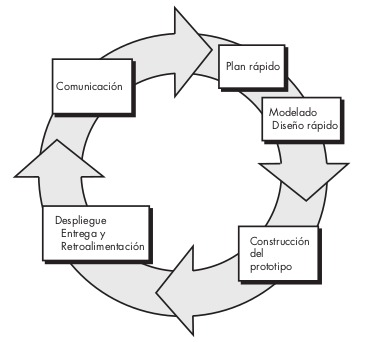
\includegraphics[width=7cm]{./imagenes/Introduccion/Meto_Prototipos.jpeg}
    			\caption[Fases de la metodología por prototipos]{Diagrama de los fases de la metodología de prototipos evolutivos.}
    			\label{fig:metodologia}
    			\end{center}
    		\end{figure}
    		
    		Para nuestro trabajo terminal y como primera fase vamos a realizar un prototipo con el fin de evaluarlo y considerar mejoras para la siguiente evolución del mismo. No se conoce el número total de prototipos que se deban realizar y para evaluarlos será necesario implementar cada uno de estos, es importante resaltar que nuestro sistema se encuentra conformado por componentes y que en algunos casos existe dependencia por lo que es indispensable considerar que para el correcto funcionamiento del prototipo se debe realizar un componente mucho antes que otro.
    		
    		A continuación se indica cada una de las etapas de la metodología con lo que se realizar\'a en cada una de estas: 
    		\begin{enumerate}
    		    \item Comunicaci\'on y plan r\'apido
    		        \begin{itemize}
    		            \item Reunir requerimientos del prototipo
    		            \item Componente 1
        		            \begin{itemize}
        		                \item Investigar sobre el desarrollo de extensiones en Google Chrome.
                		        \item Investigar sobre el método Chaffing and Winnowing.
        		            \end{itemize}
        		        \item Componente 2
        		            \begin{itemize}
        		                \item Investigar sobre Certificados
        		                \item Investigar sobre Autoridades Certificadoras.
        		            \end{itemize}
        		        \item Componente 3
        		            \begin{itemize}
        		                \item Investigación sobre el servidor Apache.
                                \item Analizar la arquitectura del servidor Apache
                                \item Investigación sobre la versión de Apache conveniente a modificar.
        		            \end{itemize}
        		        \item Describir el prototipo.
            		\end{itemize}
            	\item Modelado y diseño rápido
            	    \begin{itemize}
            	        \item Componente 1
            	            \begin{itemize}
            	                \item Modelar un algoritmo que genere un patrón de chaffing.
                    	        \item Modelar un algoritmo de chaffing.
                    	        \item Crear un método que reciba un certificado, una cabecera HTTP y el patrón.
                    	        \item Diseñar una cabecera HTTP modificada que pueda contener la información de autenticación 
            	            \end{itemize}
            	        
            	        \item Componente 2
            	            \begin{itemize}
            	                \item Diseñar una Base de datos para almacenar los datos del usuario y su certificado.
            	            \end{itemize}
            	        \item Componente 3
            	            \begin{itemize}
            	                \item Diseñar una API en el servicio web que permita interceptar una petición HTTP.
            	            \end{itemize}
            	        \item Diseñar una arquitectura del sistema.
            	    \end{itemize}
                \item Construcción del prototipo
                    \begin{itemize}
            	        \item Componente 1
            	            \begin{itemize}
            	                \item Implementar el algoritmo de chaffing.
            	                \item Implementar una extensión que intercepte peticiones HTTP.
            	                \item implementar un login en donde el usuario pueda iniciar sesi\'on.
            	            \end{itemize}
            	        
            	        \item Componente 2
            	            \begin{itemize}
            	                \item Implementar la Autoridad Certificadora.
            	                \item Implementar un Servidor que reciba y envíe peticiones.
            	            \end{itemize}
            	        \item Componente 3
            	            \begin{itemize}
            	                \item Implementar un servidor Apache.
            	                \item Implementar una API que reciba una petición y pueda identificarla.
            	            \end{itemize}
                    \end{itemize}
                \item Despliegue, entrega y Retroalimentaci\'on: Despu\'es de la implementación del prototipo se analizará si puede haber mejoras y si es conveniente la realización de otro prototipo evolucionando este o desechándolo.
                    
    		\end{enumerate}
    		
    		
    		
        
        \section{Organización del documento}
            Para dar inicio a este trabajo terminal, presentamos de manera breve la estructura de este reporte, con el objetivo de que el lector pueda tener un mejor entendimiento del trabajo.
             
            \subsection{Capítulo 2. Marco teórico.}
                Dado que este trabajo terminal relaciona temáticas muy enfocadas a la seguridad y aspectos web, es necesario conocer algunos conceptos e ideas fundamentales tanto para entenderlo como para conocer su funcionamiento, por lo tanto será necesario hablar del protocolo HTTP, métodos de autentificación, criptografía y acerca del método \textit{Chaffing and Winnowing} que es la parte medular de todo este trabajo; en este marco teórico se explicará de manera breve y con un enfoque directo el uso que le daremos a estos conceptos en el trabajo terminal.
             
            \subsection{Capítulo 3. Análisis.}
                Dentro de este capitulo se analiza el estudio de factibilidad tanto t\'ecnico como operativo y económico con la finalidad de conocer los recursos necesarios para la elaboración de este trabajo terminal. Se mencionan de manera resumida las herramientas a utilizar y se explica de manera general la arquitectura del sistema  y el diagrama de casos de uso general. Finalmente se muestra el análisis de los 3 componente que tenemos en el sistema.
             
            \subsection{Capítulo 4. Diseño.}
                En el tercer capítulo, no adentraremos en el desarrollo del los prototipos, es decir, se encuentran los diagramas pertinentes para poder modelar nuestro trabajo terminal y proceder a la etapa de codificación. En este capítulo se desarrollan y explican los siguientes diagramas: 'Casos de uso', 'Flujo', 'Flujo de datos', 'Clases', 'Secuencia' y 'Actividades' y se muestra la interfaz de usuario propuesta junto con los requisitos de diseño.
                
            \subsection{Capítulo 5. Desarrollo.}
                En este capítulo, mostraremos lo que hemos desarrollado para este TT1 (Componente I). Se muestra que el prototipo cumpla los requerimientos que se le impusieron en la sección de análisis.
            
            \subsection{Capítulo 6. Avances y trabajo por hacer.}
                En el último capítulo de este reporte, hablaremos de los avances que hemos logrado a lo largo de la asignatura de trabajo terminal I y además, exponemos el trabajo esperado para la asignatura de trabajo terminal II.
            
	\chapter{\textcolor{azulescom}{Marco teórico}}
	    \section{Protocolo HTTP}
    	    Desde 1990, el protocolo HTTP (Hypertext Transfer Protocol, Protocolo de transferencia de hipertexto) es el protocolo más utilizado en Internet. La versión 0.9 solo tenía la finalidad de transferir los datos a través de Internet (en particular páginas web escritas en HTML). La versión 1.0 del protocolo (la más utilizada) permite la transferencia de mensajes con encabezados que describen el contenido de los mensajes mediante la codificación MIME.

            El propósito del protocolo HTTP es permitir la transferencia de archivos (principalmente, en formato HTML). entre un navegador (el cliente) y un servidor web (denominado, entre otros, httpd en equipos UNIX) localizado mediante una cadena de caracteres denominada dirección URL. 
            
            La comunicación entre el navegador y el servidor al que se quiere acceder se realiza de la siguiente manera en la figura \ref{fig:DiagramaHTTP}:
            \begin{figure}[H]
        			\begin{center}	                  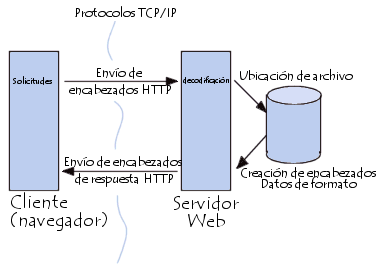
\includegraphics[width=7cm]{./imagenes/MarcoTeorico/HTTPcs.png}
        				\caption{Comunicaci\'on Cliente - Servidor en el protocolo HTTP}
        				\label{fig:DiagramaHTTP}
        			\end{center}
        	\end{figure}
        	El navegador realiza una solicitud HTTP y el servidor procesa la solicitud y después envía una respuesta HTTP. En realidad, la comunicación se realiza en más etapas si se considera el procesamiento de la solicitud en el servidor. Dado que sólo nos ocupamos del protocolo HTTP, no se explicará la parte del procesamiento en el servidor en esta sección del artículo\cite{protocoloHTTP}. 
        	\subsection{Solicitud HTTP}
        	    Una solicitud HTTP es un conjunto de líneas que el navegador envía al servidor. Comprende:
        	    \begin{itemize}
        	        \item \textbf{Una línea de solicitud: } una línea que especifica el tipo de documento solicitado, el método que se aplicará y la versión del protocolo utilizada. La línea está formada por tres elementos que deben estar separados por un espacio: el método, la dirección URL y la versión del protocolo utilizada por el cliente (por lo general, HTTP/1.0)
        	        \item \textbf{Los campos del encabezado de solicitud: } un conjunto de líneas opcionales que permiten aportar información adicional sobre la solicitud y/o el cliente (navegador, sistema operativo, etc.). Cada una de estas líneas está formada por un nombre que describe el tipo de encabezado, seguido de dos puntos (:) y el valor del encabezado.
        	        \item \textbf{ El cuerpo de la solicitud: }un conjunto de líneas opcionales que deben estar separadas de las líneas precedentes por una línea en blanco y, por ejemplo, permiten que se envíen datos por un comando POST durante la transmisión de datos al servidor utilizando un formulario. 
        	    \end{itemize}
            \subsection{Respuesta HTTP}
                Una respuesta HTTP es un conjunto de líneas que el servidor envía al navegador. Está constituida por:
                \begin{itemize}
                    \item \textbf{Una línea de estado: } una línea que especifica la versión del protocolo utilizada y el estado de la solicitud en proceso mediante un texto explicativo y un código. La línea está compuesta por tres elementos que deben estar separados por un espacio: la versión del protocolo utilizada, el código de estado y el significado del código.
                    \item \textbf{Los campos del encabezado de respuesta: } un conjunto de líneas opcionales que permiten aportar información adicional sobre la respuesta y/o el servidor. Cada una de estas líneas está compuesta por un nombre que califica el tipo de encabezado, seguido por dos puntos (:) y por el valor del encabezado.
                    \item \textbf{El cuerpo de la respuesta: } contiene el documento solicitado. 
                \end{itemize}
                
        %   %   %   %   %   %   %   %   %   
		%		                        %
		%   Certificado                 %
		%                               %
	    %   %   %   %   %   %   %   %   %
        \section{Certificado}
        Un certificado digital (X.509, v.3) es un fichero que contiene (entre otros datos) la clave pública (y privada) de una persona y está avalado (firmado electrónicamente) por una entidad de confianza o \textit{Autoridad de Certificación}.\\
        La Fabrica Nacional de Moneda y Timbre (FNMT) emite certificados digitales (los certificados del Documento Nacional de Identidad [DNI]  están emitidos por la Dirección General de la Policía - Fabrica Nacional de Moneda y Timbre [DGP-FNMT]) \cite{refCertificadosElectronicos}.\\
        El certificado digital contiene, entre otros datos, los siguientes:
        \begin{itemize}
            \item Filiación del propietario (Nombre, DNI, email).
            \item Protocolo de firma que se lleva a cabo (C,D).
            \item Autoridad de certificación que emite el certificado (FNMT).
            \item Fecha de emisión y de caducidad (2-3 años).
            \item Clave publica -privada- del propietario (\textit{K -k-}).
            \item Firma electrónica de la autoridad de certificación.
        \end{itemize}
        
        Todo certificado debe estar firmado electrónicamente por una Autoridad de Certificación (AC) para ser valido.
        Este proceso de firma lo lleva a cabo la AC a la vez que genera el certificado (Figura  \ref{fig:AC_validacion}), se lleva a cabo de la siguiente manera:
        \begin{itemize}
            \item Recopila los datos del usuario y las claves generadas por su navegador.
            \item Calcula un resumen (hash) de todos los datos recopilados.
            Firma electrónicamente el resumen anterior y lo une a los datos recopilados (Valor de la firma del certificado o Huella digital).
        \end{itemize}
        
        \begin{figure}[H]
    		\begin{center}	                  
    		    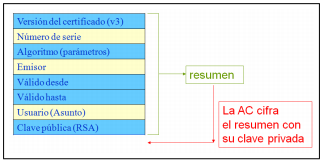
\includegraphics[width=8cm]{./imagenes/MarcoTeorico/FirmaCertificadoAC.png}
    			\caption{Firma de un certificado por una AC.}
    			\label{fig:AC_validacion}
    		\end{center}
    	\end{figure}
        
        Antes de que un certificado personal (el único que puede tener claves privadas) sea instalado en el almacén de un navegador, éste verifica que está firmado por una AC (Figura \ref{fig:AC_verificacion}) de las incluidas en su almacén de certificados (Autoridades) de la siguiente manera:
        \begin{itemize}
            \item Calcula el resumen (hash) de todos los datos recopilados del certificado, sin incluir la firma electrónica de la Autoridad Certificadora.
            \item Descifra la firma del certificado con la clave publica de la AC (debe estar en su almacén de Autoridades).
            \item Compara el resumen calculado con lo descifrado y decide sobre su autenticidad.
        \end{itemize}
        
        \begin{figure}[H]
			\begin{center}	                  
			    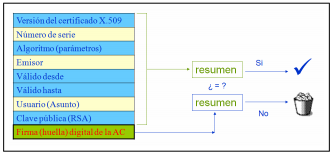
\includegraphics[width=8cm]{./imagenes/MarcoTeorico/VerificacionCertificado.png}
				\caption{Verificación de un certificado firmado por una AC.}
				\label{fig:AC_verificacion}
			\end{center}
		\end{figure}
        
        
	    %   %   %   %   %   %   %   %   %   
		%		                        %
		%   MÉTODOS DE autentificación  %
		%                               %
	    %   %   %   %   %   %   %   %   %
	    \section{Métodos de autentificación en internet.}
	    Con la evolución de la web, distintas páginas ofrecen ciertos servicios a los usuarios y con la finalidad de dar una experiencia óptima y segura, se requiere que una persona o usuario se identifique para el uso de estos servicios, es aquí donde entra en juego el papel de los métodos de autentificación. Para poder asegurar la confidencialidad de la información manejada en todos estos servicios, es necesario restringir el acceso de este, para esto se utiliza la identificación y la autenticación; la identificación es un procedimiento donde el sujeto es reconocido por algún \acrshort{id}, esto es equivalente al saber una parte de información en específico, mientras que la autenticación es el proceso de validación de si el sujeto es la persona quien dice ser al tratar de identificarse \cite{ComparisonAuthenticationMethodsResources}.\\
	    
	    Para probar una identidad, el sujeto presenta algo llamado "factor de autenticación", principalmente existen 4: 
	    \begin{itemize}
	        \item El sujeto tiene algo (Token, documento, un material específico, etc.).
	        \item El sujeto conoce algo (contraseña, login, respuesta a una pregunta, etc.).
	        \item El sujeto tiene una característica biológica (huella dactilar, ADN, etc.).
	        \item El sujeto se encuentra en un lugar en específico (dirección IP, información de un lugar en específico, etc.).
	    \end{itemize}
	    Hoy en  día, la autenticación por contraseña es el método más utilizado, más que otra cosa por su ventaja principal: su simplicidad de utilización, sin embargo, así como tiene una gran ventaja, la autenticación por contraseña también tiene muchos problemas y desventajas de seguridad.
	    
	    A continuación en el cuadro \ref{cuadro:MetododsAutentificacion}, mostraremos algunas tablas comparativas que servirán para tener una mejor perspectiva de las ventajas, desventajas, vulnerabilidades de los diferentes métodos de autenticación, entre otras cosas:
		
		\begin{table}[H]
			\centering
			\resizebox{13cm}{!} {
				\begin{tabular}{l|l|l|l|l|l|l|l|}
					\cline{2-8}
					& Recordar & \begin{tabular}[c]{@{}l@{}}Otros\\ dispositivos\end{tabular} & Acciones & Facilidad & Tiempo & Errores & Recuperación \\ \hline
					\multicolumn{1}{|l|}{Contraseñas}                                                      & 1        & 3                                                            & 2        & 3         & 3      & 2       & 3            \\ \hline
					\multicolumn{1}{|l|}{Otros recursos}                                                   & 2        & 3                                                            & 3        & 3         & 3      & 3       & 2            \\ \hline
					\multicolumn{1}{|l|}{\begin{tabular}[c]{@{}l@{}}Contraseñas \\ gráficas\end{tabular}}  & 1        & 1                                                            & 2        & 3         & 3      & 2       & 3            \\ \hline
					\multicolumn{1}{|l|}{\begin{tabular}[c]{@{}l@{}}Contraseñas \\ dinámicas\end{tabular}} & 1        & 3                                                            & 2        & 2         & 3      & 2       & 2            \\ \hline
					\multicolumn{1}{|l|}{Tokens}                                                           & 3        & 1                                                            & 1        & 2         & 2      & 3       & 1            \\ \hline
					\multicolumn{1}{|l|}{Multivariación}                                                   & 1        & 1                                                            & 1        & 3         & 2      & 2       & 1            \\ \hline
					\multicolumn{1}{|l|}{Cryptografía}                                                     & 3        & 1                                                            & 1        & 1         & 1      & 2       & 1            \\ \hline
					\multicolumn{1}{|l|}{Biométricos}                                                      & 3        & 3                                                            & 2        & 3         & 2      & 2       & 1            \\ \hline
				\end{tabular}
			}
			\caption[Aplicación de los métodos de autentificación]{Tabla comparativa de la aplicación en los distintos métodos de autentificaci\'on}
			\label{cuadro:MetododsAutentificacion}
		\end{table}
		La tabla anterior concentra las siguientes características:
		
		\begin{itemize}
			\item Recordar: Hace referencia a que tan complicado es que un usuario se acuerde de los datos necesarios para la autentificaci\'on. 
			\item Otros dispositivos: El usuario usa una entidad externa para facilitar su autentificaci\'on.
			\item Acciones: Hace referencia a que tantas acciones adicionales se deben de realizar para autentificarse.
			\item Facilidad: Simplicidad de tecnología.
			\item Tiempo: Cantidad de recursos temporales que consume el método de autentificaci\'on.
			\item Errores: Posibles errores durante la autentificaci\'on. 
			\item Recuperación: Denota la dificultad de recuperar la clave de acceso en caso de pérdida.
		\end{itemize}
		
		En el cuadro \ref{cuadro:VentajasMetodos} se muestra una tabla comparativa del nivel de seguridad en los distintos métodos de autentificaci\'on, donde 1 - baja seguridad, 2 – media seguridad y 3 – alta seguridad.
		
		\begin{table}[H]
			\centering
			\resizebox{10cm}{!} {
				\begin{tabular}{l|l|l|l|l|}
					\cline{2-5}
					& \begin{tabular}[c]{@{}l@{}}Ataque por\\ fuerza bruta\end{tabular} & Observación & \begin{tabular}[c]{@{}l@{}}Hackeo\\ indirecto\end{tabular} & Phishing \\ \hline
					\multicolumn{1}{|l|}{Contraseñas}                                                      & 1                                                                 & 1           & 1                                                          & 1        \\ \hline
					\multicolumn{1}{|l|}{Otros recursos}                                                   & 2                                                                 & 2           & 3                                                          & 3        \\ \hline
					\multicolumn{1}{|l|}{\begin{tabular}[c]{@{}l@{}}Contraseñas \\ gráficas\end{tabular}}  & 1                                                                 & 1           & 2                                                          & 2        \\ \hline
					\multicolumn{1}{|l|}{\begin{tabular}[c]{@{}l@{}}Contraseñas \\ dinamicas\end{tabular}} & 2                                                                 & 3           & 2                                                          & 2        \\ \hline
					\multicolumn{1}{|l|}{Tokens}                                                           & 3                                                                 & 3           & 3                                                          & 3        \\ \hline
					\multicolumn{1}{|l|}{Multivariación}                                                   & 1                                                                 & 1           & 3                                                          & 3        \\ \hline
					\multicolumn{1}{|l|}{Cryptografía}                                                     & 3                                                                 & 3           & 3                                                          & 3        \\ \hline
					\multicolumn{1}{|l|}{Biométricos}                                                      & 3                                                                 & 3           & 1                                                          & 1        \\ \hline
				\end{tabular}
			}
			\caption[Seguridad en los métodos de autentificación]{Tabla comparativa de la seguridad en los distintos métodos de autentificaci\'on}
			\label{cuadro:VentajasMetodos}
		\end{table}
		La tabla se enfoca principalmente en los siguientes problemas de seguridad: 
		
		\begin{itemize}
			\item Ataque por fuerza bruta: Se descifra el método de autentificaci\'on con una gran cantidad de intentos, usualmente generados por un programa.
			\item Observación: Cuando se intenta ver directamente los datos necesarios para la autentificaci\'on desde una distancia cercana hasta incluso usando binoculares, cámaras o algún otro dispositivo.
			\item Hackeo indirecto: El usuario confía sus datos del método de autentificaci\'on a terceros quienes pueden ser atacados. 
			\item Phishing: Hace referencia a programas que se hacen pasar por entidades confiables para interceptar los datos que desean.
		\end{itemize}
		
	    \textbf{Seguridad en internet}
	    En la actualidad, el incremento constante de internet ha impactado directamente en la seguridad de la información que se maneja cotidianamente y por la mayoría de usuarios. Existen infinidad de sitios donde es aplicada la seguridad, ya que sin ésta, se verían afectados todos los usuarios en  sus cuentas, pudiendo verse afectados desde un posible \Gls{Robo de Identidad} (Robo de identidad), hasta la perdida de dinero real dado que la base de algunas de éstas paginas son E-Commerce, estas paginas implican el manejo de tarjetas de crédito, paypal, etc.\\
		
		Uno de los puntos más críticos de la seguridad en Internet son las herramientas que interactúan de forma directa con los usuarios. Es común escuchar sobre fallas en los sistemas de protección de los servidores más frecuentemente utilizados, por ejemplo Apache, NGINX, IIS, etc. O en los lenguajes de programación en que son escritas las aplicaciones \cite{refSeguridadWeb}. Sin embargo, la vulnerabilidad más grande dentro de un sistema, son los ataques directos a los usuarios finales durante la autentificación.\\
	    
	    Una de las técnicas de autentificación que actualmente se usa es ''recordar la sesión'' usando las ''cookies'', en la siguiente sección, nos adentraremos en definir qué son las cookies y exponer sus vulnerabilidades.
	    
	    \section{Cookies. }
		Durante la navegación por internet, la información sobre la computadora puede ser colectada y almacenada. Ésta puede ser de carácter general sobre el equipo y puede ser también información más específica sobre los hábitos de navegación del usuario, toda esta información guardada se le conoce como \Gls{cookies}. \\
		A continuación se muestran los diferentes tipos de cookies que existen para los navegadores.
		
		\begin{itemize}
		    \item \textbf{Cookies propias:} Las cookies se gestionan desde el terminal o dominio de un mismo editor.
		    \item \textbf{Cookies de terceros:} Las cookies no son enviadas por el propio editor, sino por otra entidad.  
		    \item \textbf{Cookies de sesión:} Los datos recabados sólo se recogen mientras el usuario está navegando por la página web.
		    \item \textbf{Cookies persistentes:} Los datos continúan almacenados en el terminal y se puede acceder a ellos durante un periodo de tiempo determinados.
		    \item \textbf{Cookies técnicas:} Permiten controlar el tráfico y la comunicación de datos.		
            \item \textbf{Cookies de personalización:} Dejan a los usuarios acceder según algunas características propias que se recogen (navegador, idioma, etc.).
            \item \textbf{Cookies de análisis:} Recogen datos sobre el comportamiento de los usuarios y permiten elaborar un perfil de usuario.
            \item \textbf{Cookies publicitarias:} Recogen datos sobre la gestión de los espacios publicitarios.
        \end{itemize}
		
		Las cookies persistentes son aquellas que se almacenan en el equipo para que las preferencias personales puedan ser retenidas, ayudan a los sitios web a recordar tu información y ajustes cuando los visitas más adelante. Esto conlleva un acceso más rápido y sencillo ya que, por ejemplo, no se tiene que iniciar sesión de nuevo. Además de la autentificación, otras páginas web tienen más funciones para las cookies permanentes, como: selección de idioma, selección de tema, preferencias de menú, marca-páginas internos de la web, o favoritos.
		Muchos navegadores pueden ajustar el periodo de tiempo en que las cookies persistentes deben ser almacenadas. \cite{refCookies} \\
		
		Gracias a las cookies persistentes, las direcciones de correo electrónico aparecen por default cuando se abre el correo electrónico, o en páginas de inicio personalizadas cuando se visita en línea un comercio. Si un atacante obtiene acceso puede recopilar información personal del usuario través de estos archivos y poder robar toda información del usuario. Es fácil acceder a estas cookies y obtener fácilmente la información del usuario, por lo que es necesario que el usuario nunca deje vulnerable esta información o en su debido caso borrar cookies al término de cada sesión.
		Existen diferentes funcionalidades para las cookies, una de las más importantes es la funcionalidad de seguridad, ya que contiene información importante de los usuarios \cite{refCookies}. A continuación se muestran las diferentes funcionalidades de las cookies.
		
		\begin{itemize}
		    \item \textbf{Preferencias:} Sirven para que la página se visualice atendiendo a los gustos del usuario, como por ejemplo idioma, región o tamaño de textos.
		    \item \textbf{Seguridad:} Se encargan de autentificar a los usuarios y evitar el uso fraudulento de las credenciales por parte de terceros.
		    \item \textbf{Procesos:} Son utilizadas para el correcto funcionamiento de la página en el navegador.
		    \item \textbf{Publicitarias/Estadísticas:} Se usan para que la publicidad que se muestre sea personalizada.
		    \item \textbf{Estados de la sesión:} Obtienen información del comportamiento del usuario en una página web, como por ejemplo el tiempo que pasa en una página, los ''clicks'' que realiza o la publicidad que le aparece.
		\end{itemize}
		
		\paragraph{}
		Una vez entendido que es la autentificación y el uso que se le puede dar a las cookies, procedemos a exponer como la criptografía es de gran ayuda en la seguridad en internet y como la usaremos para este nuevo método de autentificación.
		
		
	    %   %   %   %   %   %   %   %   %
		%		                        %
		%           CRIPTOGRAFÍA        %
		%                               %
	    %   %   %   %   %   %   %   %   %
	    \section{Introducción a la Criptografía.}
	        \subsection{Criptología.}
	            Para comprender que es la criptografía, es necesario que comprendamos qué es la ''\textit{Criptología}'', palabra que proviene del griego <<\textit{kryptós}>> (oculto) y <<\textit{logos}>> (estudio). Según la Real Academia Española significa 'estudio de los sistemas, claves y lenguajes ocultos o secretos', sin embargo, brindándole un contexto a esta definición decimos que es el arte y ciencia que se encarga de diseñar sistemas para ocultar mensajes, y buscar la manera de romper dichos sistemas \cite{refCriptology}.\\
	            La criptología contiene dos ramas, las cuales son: el criptoanálisis y la criptografía. Ésta última es de vital importancia en este trabajo terminal, por lo que a continuación se explicará qué es, su historia, sus objetivos y sus usos que tiene esta rama en la actualidad.
            \subsection{Criptografía.}
                ''\textit{Criptografía}'', palabra proveniente del griego <<\textit{kryptós}>> (oculto) y <<\textit{graphos}>> (escribir), es definida por la Real Academia Española como 'el arte de escribir con clave secreta o de un modo enigmático'. Nuevamente, la definición de la RAE nos da un panorama general de lo que trata esta rama de la criptología, sin embargo, en la actualidad tenemos definiciones más extensas y precisas que nos ayudan a entender las funciones de este arte.\\
                
                A continuación, se presentan dos definiciones de la criptografía, cabe mencionar que estás definiciones están orientadas al uso de la criptografía en la informática y las telecomunicaciones actualmente.\\
                Jorge Ramio Aguirre nos brinda la siguiente definición en su libro 'Seguridad informática y criptografía' \cite{refRamioAguirre}.
                \begin{center}
                    \textit{''Rama inicial de las matemáticas y en la actualidad también de la informática y la telemática, que hace uso de métodos y técnicas con el objeto principal de cifrar, y por tanto proteger, un mensaje o archivo por medio de un algoritmo, usando una o más claves.''}
                \end{center}
                Finalmente, Menezes, Van Oorschot y Vanstone, no brindan en su libro una definición formal de lo que es la criptografía (traducción) \cite{refHandBookOfAppliedCryptography}.
                \begin{center}
                    \textit{''Estudio de técnicas matemáticas relacionadas con los aspectos de la seguridad de la información tales como la confidencialidad, la integridad de datos, la autentificación de entidad y del origen de datos. La criptografía no comprende sólo a los medios para proveer seguridad de información, sino a un conjunto de técnicas.''}
                \end{center}
                A elección del lector elegir aquella definición que le convenza más, nosotros una vez finalizado la exposición de estas definiciones de criptografía, continuaremos con una breve remembranza de la historia de esta disciplina.\\
                
                En egipto hace 4000 años, tuvo su primera aparición la criptografía, cuando un maestro egipcio escribió la historia de su señor utilizando jeroglíficos poco comunes tratando de imprimir cierta jerarquía. Este primer acercamiento a la criptografía, utilizaba las técnicas de sustitución y transposición de símbolos de una manera similar a la base del concepto general de cifrado. Posteriormente, las antiguas civilizaciones occidentales comienzan a adoptar estas técnicas para mantener determinada información oculta, principalmente con propósitos militares, diplomáticos y religiosos. Mientras la criptografía crecía alrededor del mundo, el criptoanálisis también lo hacía, con el objetivo de hallar el mensaje original a partir de un mensaje cifrado, sin conocer el método utilizado \cite{refSandra} \cite{refCriptografia}.\\
                
                El la historia conocida después de lo antes mencionado, existe un punto crucial en el desarrollo de la criptografía tal y como la conocemos hoy en día hasta la llegada de las computadoras. Este punto fue la Segunda Guerra Mundial, en donde se construyeron máquinas de cifrado mecánicas y electromecánicas que aceleraban el proceso de cifrado y descifrado. Los alemanes desarrollaron la famosa máquina 'Enigma', que precisamente mediante unos rotores automatizaba el proceso de cifrado y descifrado de mensaje, brindándole al ejército una ventaja considerable en la inversión de tiempo en la comunicación.
                
            \subsubsection{Criptografía moderna.}
                En la actualidad, el término \textit{'criptografía moderna'} hace alusión al desarrollo de esta ciencia en las áreas de la teoría de la información y las comunicaciones. Claude Shannon, considerado por muchos como el padre de la criptografía matemática, en su libro ''Sistemas secretos'' estableció las bases para las implementaciones de los algoritmos actuales a mediados de los años 50s \cite{refCriptografia}.\\
                En los años 70s, el público general tuvo acceso al trabajo de Claude, además surgió la llegada de las computadoras y la publicación el primer borrador del algoritmo de criptografía simétrica DES, el cual fue el primer algoritmo público, basado en técnicas matemáticas y criptográficas modernas. Todo ello representó los cimientos para un rápido crecimiento en la criptografía, hasta eventualmente llegar a otro hecho sumamente relevante que determinó gran parte de las transacciones que realizamos hoy en día en internet. Dicho hecho fue el artículo de las nuevas direcciones de criptografía hecho por Whitfield Diffie y Martin Hellman, el cual trataba de un nuevo método para distribuir llaves, que eventualmente se llamaría criptografía asimétrica.
                
            \subsection{Objetivos de la criptografía.}
                Algunos de los objetivos que se busca con la implementación de la criptografía para la seguridad de la información son los siguientes:
                \begin{itemize}
                    \item \textbf{Confidencialidad:} este objetivo, también conocido como privacidad de la información, implica mantener en secreto una determinada información, por tanto, sólo aquellas personas que estén autorizadas tendrán acceso a ella.
                    \item \textbf{Autentificación:} este objetivo, implica hablar de la corroboración de la identidad de una entidad, por tanto, asegura que la entidad de donde la información es originada pueda ser identificada.
                    \item \textbf{Integridad:} este objetivo asegura que determinada información no haya sido alterada por personas no autorizadas o por cualquier otro medio no conocido.
                    \item \textbf{No repudio:} este objetivo previene que una entidad niegue un envío de información de un acuerdo preestablecido.
                \end{itemize}
            \subsection{Usos de la criptografía.}
                Los usos que tiene la criptografía son muy variadas, dependiendo del ámbito donde se está aplicando. Las siguientes usos, son sólo algunas de los tantos que hay y provienen de distintos objetivos que tiene la criptografía aplicada a la seguridad de la información \cite{refCriptografia}.
                \begin{itemize}
                    \item \textbf{Autorización:} permiso concreto, de una parte o entidad, para el acceso o la realización de una tarea especifica.
                    \item \textbf{Validación:} proveer una autorización para el uso o la manipulación de información o recursos.
                    \item \textbf{Control de acceso:} restricción de acceso a la información o recurso.
                    \item \textbf{Certificación:} respaldo de información por una entidad externa de confianza.
                    \item \textbf{Confirmación:} acuse de recibo a servicios que han sido dados.
                    \item \textbf{Anonimato:} ocultamiento de la identidad de una entidad.
                \end{itemize}
                
            \subsection{Criptografía simétrica y asimétrica.}
                Anteriormente en la historia de la criptografía, se hizo una rápida mención del nacimiento de estos dos métodos de cifrado, en esta sección se explicará más profundamente sus funciones con el fin de que el lector conozca un poco más y entienda porque hemos decidido utilizar determinado método para cumplir con los objetivos de este trabajo.
                
                \subsubsection{Criptografía simétrica.}
                En la criptografía simétrica, tanto el emisor como el receptor comparten una única llave secreta para cifrar y descifrar la información que se deseé transmitir. Esto implica que ambas partes de la comunicación deben tener un acuerdo antes de que se realice la comunicación. La seguridad de este tipo de algoritmos radica en mantener segura la llave secreta, por tanto, si ésta es revelada, cualquiera con acceso a ella puede descifrar el mensaje. Por estas razones, este tipo de criptografía puede ser visto como "criptografía de llave privada". Algunos de los algoritmos más famosos de criptografía simétrica son: DES (Data Encryption Standard), TripleDES, AES (Advanced Encryption Standard) y IDEA (International Data Encryption Algorithm) \cite{refCriptografia}.\\
                En el esquema de la Figura \ref{fig:criptoSimetrica}, se muestran los pasos que sigue un protocolo de criptografía simétrica. Definamos 'A' como una entidad que pretende enviar un mensaje a otra entidad llamada 'B'. Luego entonces, ambas partes acordarán una 'Llave Secreta' con la que 'A' cifrará el mensaje utilizando un algoritmo establecido, mandando el resultado (Texto Cifrado) a 'B' que descifrará el mensaje con la misma llave y algoritmo que 'A'.
                
                \begin{figure}[H]
        			\begin{center}	                  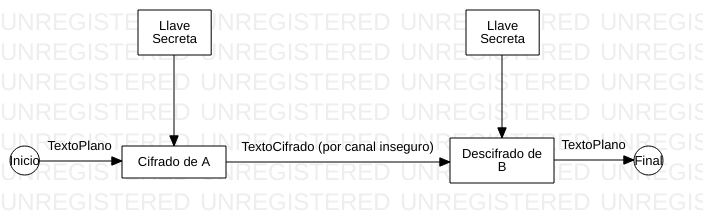
\includegraphics[width=14cm]{./imagenes/MarcoTeorico/cripto_simetrica.png}
        				\caption{Esquema del protocolo de criptografía simétrica.}
        				\label{fig:criptoSimetrica}
        			\end{center}
        		\end{figure}
        		
        		\subsubsection{Criptografía asimétrica.}
        		La  criptografía  de  clave  pública  fue  inventada  en 1976  por  los  matemáticos  Whitfield Diffie y Martin Hellman y es la base de la criptografía moderna. \\
        		En los algoritmos de criptografía asimétrica, el receptor posee una llave pública y una llave privada para poder descifrar los mensajes. Las claves privadas deben ser conocidas únicamente por su propietario, mientras que la correspondiente clave pública puede ser dada a conocer abiertamente. Si un usuario quiere enviar a otro un mensaje de forma que sólo el receptor pueda entenderlo, lo codificará con la clave pública del receptor y éste utilizará su clave privada, que solo él tiene, para poder leerlo. Dicho esto, podemos llamar llave de cifrado a la llave publica y llave de descifrado a la llave privada, siendo ambas totalmente diferentes una de la otra. Algunos de los algoritmos más famosos de criptografía asimétrica son: RSA y ElGamal \cite{refCriptografia}.\\
        		La criptografía asimétrica está basada en la utilización de números primos muy grandes. Si multiplicamos entre sí dos números primos muy grandes, el resultado obtenido no puede descomponerse eficazmente, es decir, utilizando los métodos aritméticos más avanzados en las computadoras más avanzadas sería necesario utilizar durante miles de millones de años tantas computadoras como átomos existen en el universo. El proceso será más seguro cuanto mayor sea el tamaño de los números primos utilizados.\\
        		
        		En el esquema de la Figura \ref{fig:criptoAsimetrica}, se muestran los pasos que sigue un protocolo de criptografía asimétrica. Definamos 'A' como una entidad que desea enviar información a otra llamada 'B'. Luego entonces, 'B' enviará a 'A' su llave pública para que 'A' cifre la información utilizándola. Cuando la información (Texto Cifrado) haya viajado a través del canal inseguro para que 'B' la reciba, 'B' descifrará el Texto Cifrado con su llave privada.
        		
        		\begin{figure}[H]
        			\begin{center}	                  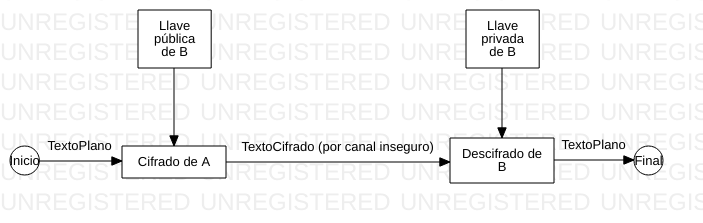
\includegraphics[width=14cm]{./imagenes/MarcoTeorico/cripto_asimetrica.png}
        				\caption{Esquema del protocolo de criptografía asimétrica.}
        				\label{fig:criptoAsimetrica}
        			\end{center}
        		\end{figure}
        		
    		\textbf{Algoritmo RSA.}\\
    		\textit{RSA} es el algoritmo de cifrado asimétrico más popular en la actualidad. Creado por Ron Rivest, Adi Shamir y Leonard Adleman y publicado en el año 1977. El algoritmo es considerado seguro, en tanto sean utilizadas llaves de longitud suficientemente seguras (se siguen utilizando llaves de 1024 bits, pero ya se recomienda al menos una longitud de 2048). El algoritmo sirve tanto para cifrar y descifrar, así como también para la generación de firmas digitales. Es, en la actualidad, ampliamente utilizado en protocolos de comercio electrónico. La seguridad \textit{RSA} está basada en la dificultad de realizar el \textit{factoreo} de números grandes. La llave privada y la publica son generadas o calculadas en función de un par de números primos, del orden de los 200 dígitos o más grandes aún \cite{refCriptografia}. \\
    		Al describir ya concretamente al algoritmo, se establece que para la generación del para de llaves (Llave publica y privada) se deberán seleccionar dos números primos grandes aleatorios, $p$ y $q$, y se calculara $n$ como su producto:
    		
    		\begin{center}
    		    $n=pq$
    		\end{center}
    		
    		La llave de cifrado, $e$, será elegida también de manera aleatoria, tal que $e$ y $(p-1)(q-1)$ sean primos relativos.\\
    		La llave de descifrado $d$ será obtenida despejando la ecuación:
    		
    		\begin{center}
    		    $ed=1 mod (p-1)(q-1)$
    		\end{center}
    		
    		En otras palabras, o mejor dicho, en otros símbolos:
    		
    		\begin{center}
    		    $d=e^{-1} mod ((p-1)(q-1))$
    		\end{center}
		    
		    Los números $e$ y $n$ componen la llave privada; el número $d$ corresponde a la llave privada; $p$ y $q$ serán descartados pero no revelados.\\
		    A la hora de cifrar un mensaje $m$, éste deberá ser dividido en bloques más pequeños que $n$ y cada parte del texto-cifrado, $c$, será obtenida mediante:
		    
		    \begin{center}
		        $c_i=m^{e}_imodn$
		    \end{center}
		    
		    Para el descifrado, cada parte o bloque del texto-cifrado se tomará para calcular:
		    
		    \begin{center}
		        $m_i=c^{d}_imodn$
		    \end{center}
		    
		    El patrón con el que se genera el código \textit{Chaffing} no puede viajar a través de la red visible para cualquier entidad que quiera obtener dicha petición, por lo que, debemos cifrarlo con algún algoritmo confiable.\\
		    El algoritmo RSA nos proporciona esa seguridad, debido a que es un cifrado asimétrico con el cual podemos cifrar el patrón con la llave publica del servicio. Una vez que la petición cifrada llegue al servicio, este será capaz de descifrar dicho mensaje con su llave privada, para así poder ver el mensaje original.\\
        		
	    
	    %   %   %   %   %   %   %   %   %   
		%		                        %
		%               C&W             %
		%                               %
	    %   %   %   %   %   %   %   %   %
            
            \subsection{Criptografía a nivel de aplicación.}
                La criptografía a nivel de aplicación se entiende como aplicaciones o programas informáticos que hacen uso de diferentes técnicas criptográficas. Al hablar de criptografía en el nivel de aplicación, también podría considerarse a los protocolos criptográficos de alto nivel, los cuales determinan como han de comunicarse ambas partes, que algoritmos usar, define formatos, etc \cite{refCriptografia}.
                
                \subsubsection{SSL/TLS.}
                Secure Sockets Layer (SSL) provee servicios de seguridad entre la capa TCP y las aplicaciones que hacer uso de esa capa. Actualmente, la sucesora de SSL es TLS (Transport Layer Service), sin embargo, lo acuñado que está el término SSL hace que se use indistintamente para referirse a TLS, aunado a ello, las diferencias entre la última versión de SSL (SSL3.0) y la primera versión de TLS (TLSv1) son menores, por lo que en el desarrollo de este reporte, utilizaremos el término SSL/TLS.\\
                
                SSL/TLS provee entonces confidencialidad, lográndola con criptografía asimétrica y controlando la integridad de los datos utilizando un MAC (Message Authentication Code).\\
                
                El proceso de comunicación del protocolo establece, como primer paso, la negociación de ambas partes de los algoritmos a utilizar. Luego, procede al intercambio de llaves públicas y a la autentificación basada en certificados digitales para, finalmente, cifrar de manera simétrica los datos o información a transferir \cite{refCriptografia}.\\
                
                En nuestro trabajo, usaremos SSL/TLS para brindar confidencialidad al canal de comunicación entre la extensión y el servidor autentificador. Esto se explicará más a detalle en el análisis del Componente II.
                
                \subsubsection{OpenSSL}
	            OpenSSL es un proyecto de código abierto que implementa funciones criptográficas sin limitaciones dentro de una librería y que provee diversas herramientas útiles. OpenSSL actualmente implementa SSL2.0, SSL3.0 y TLSv \cite{refCriptografia}.\\
	            
	            Dentro de las herramientas que tiene se encuentran: 
	            \begin{itemize}
	                \item Crear y manejar llaves privadas, públicas y parámetros.
	                \item Realizar operaciones criptográficas de llave pública.
	                \item Calcular hash de algún mensaje.
	                \item Cifrar y descifrar con algoritmos simétricos.
	                \item Crear certificados X.509 (CSRs y CRLs).
	            \end{itemize}
	            
	            Esta última herramienta, es la que usaremos para este trabajo terminal. Se creará un certificado de cada usuario a partir de sus datos de inicio de sesión para autentificarlo en los servicios web en donde quiera acceder. Esto se explicará más a detalle en el análisis del Componente II.
	            
	    \paragraph{}
	    Ahora que se ha expuesto el uso de la criptografía en este trabajo, procedemos a platicar acerca del método \textit{Chaffing and Winnowing} y cómo se implementará en este trabajo.
	   
	    \section{Chaffing and Winnowing.}
	    \subsection{Historia}
	    Chaffing and Winnowing es una técnica que logra confidencialidad sin usar ning\'un proceso de cifrado para el env\'io de datos sobre un canal inseguro. El nombre \textbf{Chaffing and Winnowing} el nombre proviene de la agricultura: D\'espues de que el grano ha sido cosechado y trillado es mezclado con paja fibrosa no comestible. La paja y el grano son separados por el movimiento de las hojas y la paja es descartada.
	    \'Esta t\'ecnica fue creada por Ron Rivest y fue publicada en un articulo en l\'inea el 18 de Marzo de 1998 \cite{refCryptohraphyWithoutEncryption}.
	    A\'unque parece ser similar a un cifrado tradicional o esteganograf\'ia, chaffing and winnowing no puede ser clasificado como uno de ellos.\\
	    \'Esta t\'ecnica permite el env\'io de datos evitando la responsabilidad del cifrado de su contenido. Cuando se usa chaffing and winnowing, el emisor transmite el mensaje sin cifrar (texto plano). Aunque el emisor y el receptor comparten una llave, ellos la usan s\'olo para autentificar. Sin embargo, una tercera parte puede hacer su comunicaci\'on confidencial durante el env\'io simult\'aneo de mensajes especialmente mensajes diseñados a través del mismo canal.
	    
	    \subsection{¿Qu\'e es Chaffing and Winnowing?}
	    
	    \paragraph{}
        Chaffing and Winnowing es un nuevo esquema establecido por Rivest en 1998. Este esquema ofrece confidencialidad para el contenido de un mensaje sin involucrarse con cifrado ni estenografía \cite{refCriptografia}.
	    
        El proceso \textbf{Chaffing} no hace uso de un cifrado por lo que no tiene una ''clave de cifrado''. Este proceso consiste en agregar paquetes inv\'alidos (Informaci\'on innecesaria) al mensaje a enviar, haciendo que el mensaje viaje seguro a la vista de todos los posibles ''atacantes''.\\
        El proceso de \textbf{Winnowing} no emplea alg\'un tipo de cifrado, por lo que al igual que el proceso chaff no tiene una ''clave de descifrado''. Intentando regular la confidencialidad que provee un cifrado damos paso a la esteganograf\'ia y el proceso de winnowing \cite{refCryptohraphyWithoutEncryption}.
        
        \paragraph{}
        Existen dos partes en el envio de mensajes con winnowing: Autentificaci\'on (Agregando MACs) y agregando paquetes chaff. Nosotros nos enfocaremos mas al uso de paquetes chaff para el env\'io seguro de informaci\'on, ya que, el receptor es quien remueve los paquetes chaff para obtener el mensaje original. 
        
        \paragraph{}
        Los siguientes esquemas explican como es que se lleva a cabo el proceso de \textbf{Chaffing and Winnowing} en diferentes escenarios.
        
		\paragraph{}
		\textbf{Escenario 1:} Alice se est\'a comunicando con Bob en un solo camino de comunicación sobre un canal inseguro y Charles agrega los paquetes de Chaff.\\
		\begin{figure}[!htb]
			\begin{center}	                  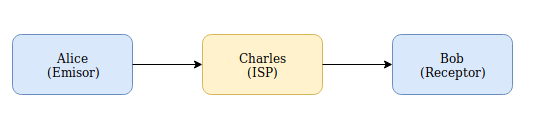
\includegraphics[width=14cm]{./imagenes/MarcoTeorico/chaffProcess.png}
				\caption{Charles agrega los paquetes inválidos.}
			\end{center}
		\end{figure}
		
		En el escenario anterior Alice y Bob se están comunicando mutuamente por un canal de comunicación no seguro, en donde son enviados paquetes no cifrados. Alice y Bob comparten la llave de autentificación la cual será usada para el proceso de autentificación. Cuando Alice envía un mensaje a Bob, su mensaje es autenticado de su lado y es enviado a Charles antes de ser enviado a Bob. Charles agrega los paquetes chaff a la secuencia transmitida por Alice, al agregar los paquetes chaff, Charles provee confidencialidad para la comunicación entre Alice y Bob. Pero donde Charles no conoce la llave secreta compartida entre Alice y Bob. Por lo que el proceso de chaffing no necesita ningún conocimiento de la llave secreta de autentificación compartida.
		\paragraph{}
		\textbf{Escenario 2:} Alice se comunica con Bob en un camino de comunicación inseguro y en el cual Charles no agrega los paquetes chaff si no que multiplexa los flujos de las dos partes (David y Alice). Este escenario es diferente al anterior, ya que se multiplexa el flujo de datos de Alice y Bob con el flujo de datos de David y Jane, y cuando el paquete llega a Bob el flujo de paquetes de David hacia Jane es el chaff de Bob y es descartado y vice versa para Jane.
		
		\begin{figure}[H]
			\begin{center}	                  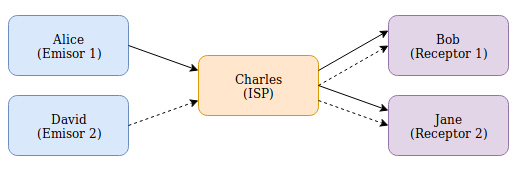
\includegraphics[width=14cm]{./imagenes/MarcoTeorico/escenario2.png}
				\caption{Charles no agrega los paquetes pero multiplexa los flujos.}
			\end{center}
		\end{figure}
		
		\paragraph{}
		\textbf{Escenario 3:} Alice se comunica con Bob en un canal de comunicación inseguro y Alice no agrega los paquetes chaff. En este escenario, Alice desarrolla la autentificación de sus mensajes, por lo que Alice aplica chaffing para autentificar los mensajes y producir una secuencia de paquetes que serán transmitidos a Bob por la vía de Charles. Bob lleva a cabo el proceso de winnowing para recuperar el mensaje original.
		
		\subsection{Objetivo de Chaffing and Winnowing}
		
		\paragraph{}
		El objetivo de seguridad del esquema de chaffing-and-winnowing es proporcionar privacidad en un entorno simétrico. 
        Desde un punto de vista de seguridad, este esquema debe tratarse simplemente como un esquema de cifrado simétrico. Hay algunos procesos de ''cifrado'' que toman un mensaje y crean un ''texto cifrado'', y algún proceso de ''descifrado'' toma el texto cifrado y recupera el mensaje, ambos operando bajo una clave secreta en com\'un. (Para el esquema Chaffing and Winnowing es la clave para el MAC). Estos procesos no se implementan de manera ''habitual'', pero, de manera abstracta, deben existir, de lo contrario no se logra la privacidad  \cite{refRivestSeguridad} \cite{refEncontrarLuegoAdivinar}.  
        \begin{center}
            \textit{''No es una propiedad de seguridad novedosa, sino un conjunto novedoso de restricciones en los procesos dirigidos a lograr una propiedad de seguridad estándar''\\
            ''Encontrar-luego-adivinar''. Extensión más directa al caso simétrico de la noción de indistinguibilidad.}
        \end{center}
		
		Haciendo uso de \textbf{Chaffing and Winnowing} se asegura que los adversarios no obtengan información del mensaje transmitido a lo largo de un canal de comunicación inseguro entre dos partes. \\
		Rivest propone un esquema, el cual cuenta con tres partes principales \cite{refCryptohraphyWithoutEncryption}.
		\begin{enumerate}
		    \item \textbf{Autentificación} Es el proceso de descomponer el mensaje original en un paquete más pequeño y complementar cada paquete con un código de autentificación de mensaje (MAC).
		    \item \textbf{Chaffing} Es el proceso de agregar paquetes inválidos (Chaff packets).
		    \item \textbf{Winnowing} Es el proceso de remover paquetes Chaff para obtener el mensaje original en texto plano.
		\end{enumerate}
		
		\subsection{¿Cómo funciona?}
		
		\paragraph{}
		El esquema de Chaffing and Winnowing deja que cada paquete conste de: 
		\begin{itemize}
		    \item Un número de serie
		    \item Contenido del paquete
		    \item Código de autentificación del mensaje
		\end{itemize}
		Cuando son enviados los paquetes, el mensaje con el texto plano se descompone en pequeños paquetes los cuales contienen datos y el tamaño del paquete original. Entonces, el emisor (Alice) usa el algoritmo de \textbf{código de autentificación de mensaje} (MAC) para generar el valor MAC para ser agregado al paquete y el cual se basa en el número de serie, contenido del paquete y la llave autentificación. La Figura \ref{fig:ChaffingSalidaPaquetes}, muestra la salida del paquete después del proceso de autentificaci\'on.
		\begin{figure}[H]
			\begin{center}	                  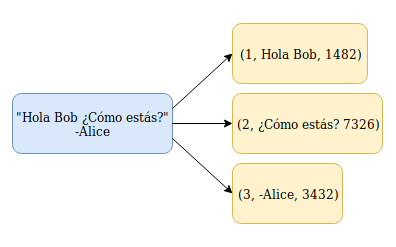
\includegraphics[width=7cm]{./imagenes/MarcoTeorico/descomposicionChaffing.png}
				\caption{Secuencia de Chaffing después del proceso de autentificación.}
				\label{fig:ChaffingSalidaPaquetes}
			\end{center}
		\end{figure}
		Esta secuencia de paquetes es enviada a Charles (ISP) para llevar a cabo el proceso de Chaffing. Charles agrega paquetes chaff a la secuencia de paquetes antes de ser enviados por medio del canal de comunicación y ser recibidos por Bob. \\
		Existen dos maneras donde Charles puede enviar la secuencia de chaff hacia Bob. La primera es enviando aleatoriamente mezclados los paquetes chaff para formar una secuencia y la otra manera es enviarlos de manera ordenada por el n\'umero de serie seguido del contenido del mensaje. En la Figura \ref{fig:ManerasChaffing}, se muestra cómo es el proceso de chaff en esta secuencia.
		\begin{figure}[H]
         \centering
          \subfloat[Primera manera]{
           \label{f:Primera manera}
            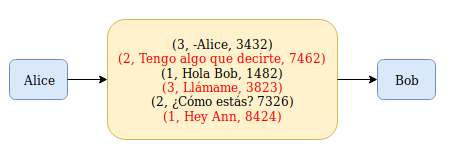
\includegraphics[width=0.5\textwidth]{./imagenes/MarcoTeorico/firstway_Chaff.png}}
          \subfloat[Segunda manera]{
           \label{f:Segunda manera}
            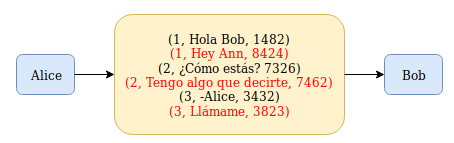
\includegraphics[width=0.5\textwidth]{./imagenes/MarcoTeorico/secondway_Chaff.png}}
         \caption[Formas del proceso de chaff]{Las dos maneras para el proceso de chaff pueden ser utilizadas. Los paquetes chaff son los mensajes de color rojo.}
         \label{fig:ManerasChaffing}
         \label{f:Enfoques}
        \end{figure}
		Una vez que la secuencia de chaff llega a Bob, el último proceso es Winnowing. Bob determina la secuencia del mensaje que es válida del paquete chaff usando una función hash para el contenido de cada paquete y la llave de autentificación para re-calcular el MAC y compararlo contra el MAC del paquete recibido, si la comparación falla, el paquete chaff es descartado. Si la comparaci\'on es valida, entonces el paquete es parte del mensaje original. En la Figura \ref{fig:ChaffingWinnowing}, se muestra el proceso completo de Chaffing and Winnowing \cite{refCryptohraphyWithoutEncryption}.

		\begin{figure}[H]
			\begin{center}	                  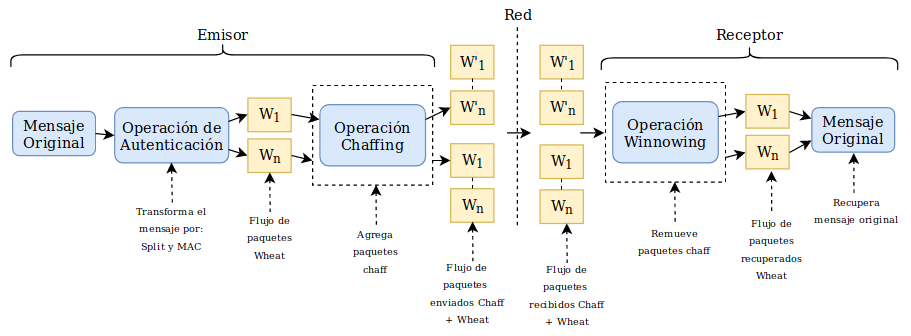
\includegraphics[width=14cm]{./imagenes/MarcoTeorico/chaff_winn.png}
				\caption{Visión general del proceso Chaffing and Winnowing.}
				\label{fig:ChaffingWinnowing}
			\end{center}
		\end{figure}
        
        \subsection{Propiedades de Chaffing and Winnowing}
        
        \paragraph{}
        \begin{itemize}
		    \item La técnica de Chaffing y Winnowing no depende de la fuerza del esquema de cifrado para proporcionar confidencialidad debido al hecho de que es muy difícil distinguir la informaci\'on \'util de los paquetes chaff sin la clave secreta. Por lo tanto, la dificultad de distinguir la informaci\'on \'util del chaff proporciona confidencialidad al esquema.
		    \item La operación de Chaffing puede ser realizada por un tercero, ya que la clave secreta compartida no es necesaria en el proceso del mismo.
		    \item Los paquetes de Chaff no tienen que contener datos aleatorios, ya que uno podría usar un mensaje válido con una clave secreta diferente para hacer el paquete de Chaff. Cuando el receptor recibe esos paquetes de Chaff, se verán como paquetes de Chaff, ya que la clave que se usa para volver a calcular el Chaff es diferente de la que los hace.
		\end{itemize}
		
		\subsection{All-or-Nothing and the Package Transform (AONT)}
        
        All-or-Nothing and the Package Transform es una variación dentro de la tecnica Chaffing and Winnowing, donde se mejora la eficiencia de su esquema original. AONT es la transformación de pre-procesamiento que permite a las partes enviar más datos (en términos de bit) por paquete en lugar de solo uno. Este pre-procesamiento es una transformación sin cifrado que toma el mensaje de texto sin formato y produce un mensaje empaquetado que luego se procesa de la manera normal de Chaffing and Winnowing \cite{refAONT}. Las definiciones de la transformación AONT son las siguientes:
        
        \begin{enumerate}
            \item El algoritmo de transformación es \textbf{reversible}: Dado el bloque de mensaje transformado, el receptor puede obtener el mensaje de texto sin formato original.
            \item El algoritmo de transformación y su inverso son \textbf{computables} de manera eficiente: Lo que significa que es computacionalmente factible recrear el texto original dada la llave privada y recibir todos los paquetes con éxito.
            \item La transformación no es \textbf{computacionalmente factible}: Esto significa que si se ha recibido parte del paquete de la transmisión, cualquiera que esté intentando leer el mensaje no puede hacerlo ya que la transformación \textbf{AONT} requiere que se reciba todo el mensaje, de lo contrario no entrega nada.
            \item La transformación es una \textbf{técnica sin cifrado}: La técnica de pre-procesamiento no tiene llaves y no hay una llave secreta compartida involucrada en la operación. Cualquier persona que haya recibido todos los mensajes transformados del paquete puede recuperar el mensaje de texto original.
        \end{enumerate}
        
        \paragraph{}
        \textbf{¿Cómo funciona AONT?}
        
        \paragraph{}
        Supongamos que el mensaje de entrada es el siguiente: $m_{1},m_{2},...,m_{n}$.\\
        Seleccionamos una llave aleatoria $K'$ el cual se usará para la función del paquete de transformación.\\
        Se calcula la secuencia transformada ${m'}_{1}, {m'}_{2},...,{m'}_{s}$ para ${s'}=s+1$ como se muestra a continuación:\\
        Tenemos:
        \begin{center}
            $m_{i} \otimes E(K',i)$ for  $i=1,2,3,...,s$
        \end{center}
        También:
        \begin{center}
            $m'_{s'}=K' \otimes h_{1} \otimes h_{2} \otimes ... \otimes h_{s}$
        \end{center}
        
        Donde:
        \begin{center}
            $h_i=E(K_0,m'_i \otimes i)$ for $i=1,2,...,s$
        \end{center}
        
        Donde $K_0$ es una llave conocida pública fija.\\
        Para que el receptor en el otro extremo obtenga el $K_0$, el cual es la llave para el uso de \textbf{AONT}, el receptor realiza el siguiente cálculo:
        
        \begin{center}
            $K'=m'_s \otimes h_1 \otimes h_2 \otimes ... \otimes h_s$
        \end{center}
        \begin{center}
            $m_i=m'_i \otimes E(K',i)$ for $i=1,2,...,s$
        \end{center}
        
        \paragraph{}
        AONT toma el mensaje de texto sin formato de entrada y los transforma, luego crea un bloque para almacenar los mensajes transformados antes de pasar al proceso de autentificación. Después, se genera el paquete Chaff (la cantidad de paquetes Chaff no tiene que ser igual a los paquetes de la informaci\'on \'util).\\
        Esta técnica produce una menor sobrecarga que la sugerencia número 1. El AONT ofrece más confidencialidad al esquema de Chaffing and Winnowing, ya que el adversario debe recibir todo el bloque de mensajes de transformación e identificar correctamente todo el paquete de la informaci\'on \'util para obtener el mensaje de texto original. La Figura \ref{fig:C&W_AONT}, muestra la descripción general de Chaffing y Winnowing si se agrega la función AONT \cite{refAONT}.
        
        \begin{figure}[H]
			\begin{center}	          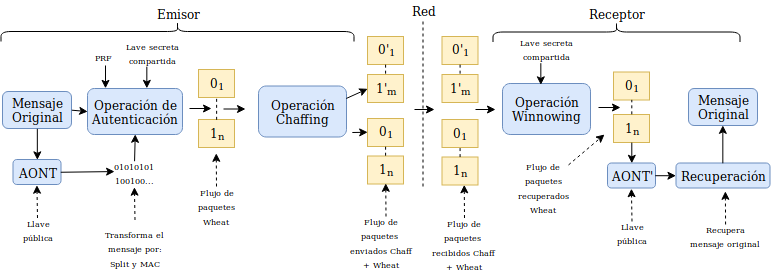
\includegraphics[width=14cm]{./imagenes/MarcoTeorico/chaffVsCrypto.png}
				\caption{Proceso de Chaffing and Winnowing junto con AONT.}
				\label{fig:C&W_AONT}
			\end{center}
		\end{figure}
		
        \textbf{¿Cómo AONT puede hacer la diferencia?}\\
        \begin{enumerate}
            \item Requiere menos ancho de banda al transferir paquetes, ya que se pueden transferir más bits en un paquete en lugar de un bit por paquete.
            \item Los paquetes Chaff son más fáciles de generar, ya que AONT transforma el mensaje de texto plano en bits aleatorios.
            \item La distinción entre Chaffing and Winnowing es más difícil: Si el adversario va a ejercer fuerza bruta en los paquetes, la tarea se ralentizará por el factor del número de bloque de mensajes. Dado que el bloque de mensaje de información adicional se mezcla aleatoriamente dentro de los flujos de paquetes de Chaffing and Winnowing, sin saber que es muy difícil que el bloque adicional proporcione la posibilidad de elegir el bloque de mensaje correcto de los paquetes para obtener el texto plano original.
        \end{enumerate}
        
        \subsection{Comparando Chaffing and Winnowing contra Cifrado y Esteganograf\'ia}
        
        En esta sección explicaremos porque Chaffing and Winnowing no puede ser clasificado como una técnica de cifrado o Estenografía.\\
        
        \subsubsection{Chafing and Winnowing vs Cifrado}
        
        Nosotros podríamos clasificar Chaffing and Winnowing como un método de cifrado, pero volvamos a recordar el principio de un Cifrado.
        El principal objetivo de un cifrado es ocultar el mensaje en texto plano de tal manera que oculta su contenido con el uso de una clave de cifrado para el texto cifrado.
        Por otro lado, en el esquema original de Chaffing and Winnowing, una llave compartida es usada con el fin de autentificar la validación de los paquetes ya sea del emisor o del receptor. Además, Chaffing and Winnowing no hace uso de ninguna técnica de cifrado para ocultar el contenido de un mensaje y que nadie pueda ver dicho mensaje, solo aquellos con la llave correspondiente pueden determinar que paquetes contienen la información valida. En la figura \ref{fig:C&W_AONT}, se muestra como se puede ver el esquema Chaffing and Winnowing como una técnica de cifrado. \\
        
        Chaffing y Winnowing pueden verse como \textbf{un tipo especial de esquema de cifrado simétrico}, ya que la operación \textbf{chaffing} es similar al ''proceso de cifrado''. En la operación de chaffing, el texto cifrado se crea para producir un paquete de la informaci\'on \'util no válido que se envía al receptor. Luego, el receptor realiza el ''proceso de descifrado'', que implica descartar el paquete de desperdicios y recuperar el mensaje original. Ambas operaciones operan bajo una llave secreta común que se usa para derivar el valor MAC.\\
        
        Pero la diferencia es, \textit{Chaffing y Winnowing} dos partes que no buscan lograr la confidencialidad. El emisor comparte una clave secreta con el receptor para que el receptor pueda usar la clave secreta para autentificarse (si se afirma que el mensaje recibido proviene del remitente deseado). Pero la ganancia de confidencialidad proviene de la dificultad de distinguir el paquete Chaff del paquete de la informaci\'on \'util. Mientras que en el cifrado, la clave se utiliza para lograr la confidencialidad mediante la creación de texto cifrado que oculta el contenido del mensaje de personas \cite{refCryptohraphyWithoutEncryption}.\\
        
        Chaffing y Winnowing junto con el esquema AONT, el esquema en sí es muy parecido al cifrado, excepto que la clave que se usa en la transformación AONT, se elige aleatoriamente cada vez en lugar de fijarla. Además, el último bloque de mensajes es exclusivo o de la clave y todo el hash del bloque de mensajes está allí para garantizar que cualquier modificación en el bloque de mensajes cambiará la clave $K'$ calculado por el receptor. Por lo tanto, el último bloque de mensajes ${m'}_{s'}$ está allí solo con el propósito de autentificación. Por lo tanto, Chaffing y Winnowing con el esquema AONT no pueden ser clasificados bajo cifrado \cite{refAONT}.\\
        
        \subsubsection{Chaffing and Winnowing vs Esteganograf\'ia}
        La esteganografía trata de cómo ocultar, dentro de un mensaje público, información secreta. La agregación de información 'extra' es también un secreto, es decir, nadie externo a la comunicación sabe que en ese mensaje público se ha agregado información \cite{refCriptografia}. Un ejemplo de esta técnica de cifrado, se puede visualizar claramente en la utilización de tinta invisible en cartas. El emisor escribe una carta común y corriente con tinta visible, pero además, escribe información secreta con tinta invisible. Luego entonces, el receptor, aplicando el método correspondiente, descubrirá la información mandada con tinta invisible, pero agentes externos, ni siquiera saben la existencia de dicha información. En la actualidad, la esteganografía es muy utilizada para ocultar información en archivos de imágenes.\\
        
        Para algunas personas, Chaffing and Winnowing puede ser clasificado como una técnica esteganograf\'ia. Sin embargo, el objetivo principal de la estenografía, como se mencionó antes, es el de ocultar el mensaje original dentro de otro mensaje, por lo tanto, nadie aparte del emisor y el receptor sabrá que hay un mensaje oculto. Contrario a Chaffing and Winnowing, en donde cualquiera puede ver el contenido del mensaje, ya que este método no trata de esconderlo de los posibles atacantes. Otra diferencia es que en esteganograf\'ia el emisor tiene que ocultar el mensaje el mismo, mientras que en Chaffing and Winnowing no necesariamente es así, ya que una ''tercera parte'' puede hacerlo \cite{refChaffingVsEsteganografia}.\\
        
        Por lo tanto, Chaffing and Winnowing no puede ser considerado como esteganograf\'ia.\\
        
         Para nuestro trabajo terminal usaremos \textit{Chaffing and Winnowing}, proponiendo así un nuevo método de autentificación para servicios web. \\

	\chapter{\textcolor{azulescom}{Análisis.}}
	    
    	\section{Estudio de Factibilidad.}
    	El estudio de factibilidad es un instrumento que sirve para orientar la toma de decisiones en la evaluación de un proyecto y corresponde a la última fase de la etapa pre-operativa dentro del ciclo del proyecto. Se formula con base en información que tiene la menor incertidumbre posible para medir las posibilidades de éxito o fracaso de un proyecto, apoyándose en él se tomará la decisión de proceder o no con su implementación. Este estudio establecerá la viabilidad, si existe, del trabajo.
    	\begin{itemize}
    	    \item Factibilidad Técnica: Hace referencia a los recursos como herramientas, conocimientos, habilidades, experiencia, etc. que son necesarios para efectuar las actividades del trabajo terminal.
    	    \item Factibilidad Operativa: Se refiere a los recursos necesarios para llevar a cabo los procesos de forma eficiente , depende de los recursos humanos.
    	    \item Factibilidad Econ\'omica: Consiste en los recursos financieros necesarios para llevar a cabo la elaboraci\'on de este trabajo.
    	\end{itemize}
    	    \subsection{Factibilidad Técnica}
    	    En esta parte explicaremos detalladamente las tecnologías que usaremos. Para la elección de estas herramientas  fue necesario investigar las tecnologías que más se usan en la actualidad, además de ver las características y equipos de c\'omputo con los que contamos actualmente.
    	        \begin{table}[H]
    				\begin{tabular}{ |p{3.5cm}||p{9.5cm}|}
    					\hline
    					\rowcolor{guindapoli}
    					\multicolumn{2}{|c|}{\textbf{\textcolor{white}{Factibilidad T\'ecnica}}}\\
    					\hline
    					\cellcolor{azulclaro}Sistema Operativo & 
    					Multiplataforma \\ 
    					\hline
    					\cellcolor{azulclaro}Navegador Web &
    					Google Chrome\\
    					\hline
    					\cellcolor{azulclaro}Lenguaje de Programaci\'on &
    					JavaScript\\
    					\hline
    					\cellcolor{azulclaro}Servidor &
    					Apache 2.0\\
    					\hline
    					
    				\end{tabular}
    				\caption[Herramientas de Software]{Herramientas de Software a utilizar}
    				\end{table}
    				Además de las herramientas de software a utilizar, es necesario mencionar el equipo de hardware que utilizaremos tanto para desarrollar como para probar e implementar cada uno de los prototipos que se mencionarán a lo largo de este trabajo terminar, el cual es:
    				\begin{table}[H]
        				\begin{tabular}{ |p{3.5cm}||p{9.5cm}|}
        					\hline
        					\rowcolor{guindapoli}
        					\multicolumn{2}{|c|}{\textbf{\textcolor{white}{Equipo de hardware [1]}}}\\
        					\hline
        					\rowcolor{azulfuerte}Marca & DELL\\
        					\hline
        					\cellcolor{azulclaro}Modelo & Inspiron 5567\\ 
        					\hline
        					\cellcolor{azulclaro}Procesador &
        					Intel Core i7 7gen\\
        					\hline
        					\cellcolor{azulclaro}Tarjeta de video & 
        					Radeon (TM) R7 M445\\
        					\hline
        					\cellcolor{azulclaro}Memoria RAM &
        					16 GB\\
        					\hline
        					\cellcolor{azulclaro}Disco Duro &
        					1 TB\\
        					\hline
        				\end{tabular}
    				\caption[Equipo de Hardware 1]{Equipo de hardware a utilizar [1]}
    				\end{table}
    				\begin{table}[H]
        				\begin{tabular}{ |p{3.5cm}||p{9.5cm}|}
        					\hline
        					\rowcolor{guindapoli}
        					\multicolumn{2}{|c|}{\textbf{\textcolor{white}{Equipo de hardware [2]}}}\\
        					\hline
        					\rowcolor{azulfuerte}Marca & Asus\\
        					\hline
        					\cellcolor{azulclaro}Modelo & X550VC\\ 
        					\hline
        					\cellcolor{azulclaro}Procesador &
        					Intel Core i5\\
        					\hline
        					\cellcolor{azulclaro}Tarjeta de video & 
        					NVidia GForce 720\\
        					\hline
        					\cellcolor{azulclaro}Memoria RAM &
        					12 GB\\
        					\hline
        					\cellcolor{azulclaro}Disco Duro &
        					1 TB\\
        					\hline
        				\end{tabular}
    				\caption[Equipo de Hardware 2]{Equipo de hardware a utilizar [2]}
    				\end{table}
    				\begin{table}[H]
        				\begin{tabular}{ |p{3.5cm}||p{9.5cm}|}
        					\hline
        					\rowcolor{guindapoli}
        					\multicolumn{2}{|c|}{\textbf{\textcolor{white}{Equipo de hardware [3]}}}\\
        					\hline
        					\rowcolor{azulfuerte}Marca & HP\\
        					\hline
        					\cellcolor{azulclaro}Modelo & Pavilion g4\\ 
        					\hline
        					\cellcolor{azulclaro}Procesador &
        					Intel Core i3\\
        					\hline
        					\cellcolor{azulclaro}Tarjeta de video & 
        					Intel Sandybridge Mobile\\
        					\hline
        					\cellcolor{azulclaro}Memoria RAM &
        					6 GB\\
        					\hline
        					\cellcolor{azulclaro}Disco Duro &
        					500 GB\\
        					\hline
        				\end{tabular}
    				\caption[Equipo de Hardware 3]{Equipo de hardware a utilizar [3]}
    				\end{table}
    		Junto con las herramientas de hardware y software a utilizar es necesario mencionar una serie de servicios b\'asicos que son relevantes para el desarrollo de este trabajo terminal como lo son:
    		\begin{itemize}
    		    \item Luz Eléctrica
    		    \item Agua Potable
    		    \item Internet
    		    \item Papelería en general
    		\end{itemize}
    		Estos servicios forman parte de la factibilidad técnica ya que sin ellos no se podría realizar este trabajo terminal y por eso mismo generan un costo, dicho costo se menciona en la Factibilidad Económica.
    		
    	    \subsection{Factibilidad Operativa}
    	    Los recursos operativos de este trabajo terminal se calcularon con base en los recursos humanos con los que se cuenta y un análisis de las horas que el personal estará en operación trabajando sobre éste, el cual se muestra a continuación:
    	    
    	    \begin{table}[H]
    			\begin{tabular}{|p{1.7cm}|p{1.6cm}||p{1.6cm}||p{1.6cm}||p{1.6cm}|p{1.6cm}|p{1.6cm}|}
    				\hline
    				\rowcolor{guindapoli}
    				\multicolumn{7}{|c|}{\textbf{\textcolor{white}{Horas a trabajar en el desarrollo del trabajo terminal}}}\\
    				\hline
    				\rowcolor{azulfuerte}Mes & No. de Días & Sábado y Domingo & Días h\'abiles & Horas de trabajo por día & Horas Totales & Días laborables (8 hr.)\\
    				\hline
    				\cellcolor{azulclaro}Enero & 31 & 8 & 9 & 2 & 18 & 2\\ 
    				\hline
    				\cellcolor{azulclaro}Febrero & 28 & 8 & 19 & 2 & 38 & 4\\ 
    				\hline
    				\cellcolor{azulclaro}Marzo & 31 & 10 & 20 & 2 & 40 & 5\\ 
    				\hline
    				\cellcolor{azulclaro}Abril & 30 & 10 & 15 & 2 & 30 & 3\\ 
    				\hline
    				\cellcolor{azulclaro}Mayo & 31 & 8 & 18 & 2 & 36 & 4\\
    				\hline
    				\cellcolor{azulclaro}Junio & 30 & 10 & 8 & 2 & 16 & 2\\
    				\hline
    				\cellcolor{azulclaro}Agosto & 31 & 9 & 12 & 2 & 24 & 3\\
    				\hline
    				\cellcolor{azulclaro}Septiembre & 30 & 10 & 16 & 2 & 32 & 4\\ 
    				\hline
    				\cellcolor{azulclaro}Octubre & 31 & 10 & 20 & 2 & 40 & 5\\ 
    				\hline
    				\cellcolor{azulclaro}Noviembre & 31 & 8 & 18 & 2 & 36 & 4\\ 
    				\hline
    			\end{tabular}
    		    \caption[Horas de trabajo]{Relación de horas de trabajo estimadas para la realización de este trabajo terminal}
    		\end{table}
    	    Con esto podemos concluir que contamos suficiente tiempo para el desarrollo de este trabajo terminal, ya que las horas totales de trabajo están contempladas para cada uno de los integrantes del equipo
    	    %\end{comment}
    	    
    	    \subsection{Factibilidad Económica}
    	    Luego de haber realizado el estudio de factibilidad técnica así como el operacional es necesario tomar en cuenta un estudio de factibilidad económica el cuan desglosará todo el gasto económico realizado para la elaboración de este trabajo terminal:
    	    \begin{itemize}
    	        \item Capital Humano: Se tienen contemplados aproximadamente 36 días laborales, es decir 288 horas para la elaboración de este trabajo terminal en el cual participaremos los cuatro integrantes
    	        \item Capital Técnico: Se cuentan con las instalaciones de la escuela, así como las viviendas de cada uno de los integrantes y los equipos de cómputo correspondientes.
    	    \end{itemize}
    	    En cuanto a los costos monetarios de todo el trabajo terminal se tiene lo siguiente:
    	    \begin{itemize}
    	        \item Servicios\\
    	        En cuando a los servicios se considera un gasto mensual aproximado de \$1,600.00 que al multiplicarlo por todo el tiempo de elaboración tenemos \$ 16,000.00.
    	        \item Software \\
    	        En este caso durante todo el trabajo terminal usaremos herramientas gratuitas y la mayoría de software libre por lo que no dedicaremos una parte monetaria en el gasto de este tipo.
    	        \item Hardware\\
    	        En este caso y como se mencionó anteriormente utilizaremos los equipos de cómputo personales de cada integrante lo que da un costo aproximado total de \$ 35,000.00.
    	        \item Recursos Humanos\\
    	        Estamos estimando un gasto de \$80,000.00 por cada integrante para la elaboración de este trabajo terminal por lo que se genera un gasto total de \$320,000.00
    	    \end{itemize}
    	    Por lo que el costo final del desarrollo de este trabajo terminal es: \\
    	    \begin{center}
    	        \$371,000.00
    	    \end{center}
    	    \textbf{Conclusión} Tras analizar todo este trabajo terminal y cada una de las partes del estudio de factibilidad es pertinente decir que los integrantes no contarán con el apoyo financiero antes mencionado y que el hardware actualmente ya es propiedad de los integrantes, por lo que el trabajo terminal se califica como \textit{''Viable''} iniciando de esta manera su implementación acorde con las fechas mencionadas.
    	    %desglosar todo el gasto alv
    	    
    	\section{Herramientas a usar.}
			\subsection{Software.}
			Para el desarrollo de software de este prototipo, es necesario hacer mención de algunas de las siguientes herramientas, para tener una idea clara sobre qué herramientas estamos utilizando y porque es que las estamos utilizando:
			
			\paragraph{HTML5.}
			HTML comenzó mucho tiempo atrás con una simple versión propuesta para crear la estructura básica de páginas web, organizar su contenido y compartir información, todo esto tenía la intención de comunicar información por medio de texto. El limitado objetivo de html motivó a varias compañías a desarrollar nuevos lenguajes y programas para agregar características a la web nunca antes implementadas.   \\\\
			Dos de las opciones propuestas fueron Java y \Gls{Flash}; ambas fueron muy aceptadas y consideradas como el objetivo de la internet, sin embargo, con el crecimiento exponencial del internet, éste dejó de ser únicamente para los aficionados de los computadores y pasó a ser usado como un campo estratégico para los negocios y para la interacción social, ciertas limitaciones presentes en ambas tecnologías probaron ser una sentencia de muerte. Esta falta de integración resultó ser crítica y preparó el camino para la evaluación de un lenguaje del cual hablaremos un poco más a detalle después: JavaScript. Sin embargo, pese a su gran impacto, el mercado no terminó de adoptarlo plenamente y rápidamente su popularidad fue declinando, y el mercado terminó enfocando su atención a Flash. No fue hasta que los navegadores mejoraron su intérprete para JavaScript y la gente se empezaba a dar cuenta de las limitaciones que ofrecía Flash, que JavaScript fue implementado y comenzó a innovar la forma en la que se programaba la web. Al cabo de unos años, JavaScript, html y css eran considerados como la más perfecta combinación para evolucionar la Web. \\\\
			HTML5 es una mejora de esta combinación, lo que unió todos estos elementos. HTML5 propone estándares para cada aspecto de la Web y también un propósito claro para cada una de las tecnologías involucradas. A partir de esto, html provee los elementos estructurales, CSS se concentra en como volver esta estructura utilizable y atractiva a la vista, y JavaScript tiene todo lo necesario para brindar dinamismo y construir aplicaciones web completamente funcionales. Cabe mencionar que HTML5 funciona diferente dependiendo del navegador y la versión en la que se esté trabajando, algunos soportan más carcterísticas o diferentes funcionalidades que otros.
			
			\paragraph{CSS3.\\}
			Ya se ha mencionado anteriormente como es que HTML5 fue evolucionando a un grado de combinación de estructura y diseño, sin embargo, la web demanda diseño y funcionalidad, no solamente organización estructural o definición de secciones, la función de CSS se concentra en volver la estructura de HTML utilizable y atractivo a la vista.\\
			
			Oficialmente CSS no tiene nada que ver con HTML4, no es parte de la especificación, es de hecho, un complemento desarrollado para superar las limitaciones y reducir la complejidad de HTML. Al principio, atributos dentro de las etiquetas HTML proveóan estilos esenciales para cada elemento, pero a medida que HTML evolucionó, la escritura de códigos se volvió más compleja y html por sí mismo no pudo satisfacer más las demandas de los diseñadores. En consecuencia a esta demanda, CSS fue adoptado como la forma de separar la estructura de la presentación, y ha ido creciendo y ganando importancia, pero siempre desarrollado en paralelo enfocado en las necesidades de los diseñadores y apartado de la estructura de HTML.\\
			
			La versión 3 de CSS sigue el mismo camino, pero esta vez con un mayor compromiso. La especificación de HTML5 fue desarrollada considerando CSS a cargo del diseño, Debido a esta consideración, la integración entre HTML y CSS es ahora vital para el desarrollo web y esta razón por la que cada vez que mencionamos HTML5 también estamos haciendo referencia a CSS3, aunque oficialmente se trate de dos tecnologías completamente separadas. Las nuevas características incorporadas en CSS3 están siendo implementadas e incluidas junto al resto de la especificación en navegadores compatibles con HTML5 \cite{refElGranLibro}.
			
			\paragraph {JavaScript. \\}
			JavaScript es considerado como el lenguaje de programación de html y de la web. Es un lenguaje de programación fácil de usar y muy versátil para el ámbito de la comunicación en redes. Los programas, llamados "scripts", se ejecutan en el navegador (Mozilla, Google Chrome, Internet Explorer, etc.) normalmente consisten en unas funciones que son llamadas desde el propio html cuando algún evento sucede.\\\\
			Su primera aproximación a un uso real, fue en mayor parte para "dar vida a una página web", como dar animaciones a un botón, interacciones en tiempo real, entre otras más. 
			JavaScript fue desarrollado por \Gls{NetScape}, a partir del lenguaje Java, que en ese momento tenía mucho auge y popularidad, y su principal diferencia es que JavaScript sólo "funciona" dentro de una página html.\\
			JavaScript fue declarado como estándar del European Computer Manufacturers Association (ECMA) en 1997, y poco después, también fue estandarizado por ISO \cite{refJavaScript}. \\ 
			JavaScript es un lenguaje interpretado, usado mayormente como complemento de ciertos objetivos específicos, sin embargo, uno de las innovaciones que ayudó a JavaScript fue el desarrollo de nuevos motores de interpretación, creados para acelerar el procesamiento del código. La clave de los motores más exitosos fue transformar el código de Javascript en código máquina para obtener una velocidad de ejecución mejor que antes. Esto a la vez permitió superar viejas limitaciones de rendimiento y confirmar el lenguaje JavaScript como la mejor opción para la Web.\\
			
			Para aprovechar esta prometedora plataforma de trabajo ofrecida por los nuevos navegadores, JavaScript fue expandido en cuestión de portabilidad e integración, a la vez, interfaces de programación de aplicaciones (APIs) fueron incorporando por defecto con cada navegador para asistir a JavaScript en funciones elementales. El objetivo de esto, fue principalmente hacer disponible poderosas funciones a través de técnicas de programación sencillas y estándares, expandiendo el alcance del lenguaje y facilitando la creación de programas útiles para la Web \cite{refElGranLibro}.
			
			\paragraph{CryptoJs. \\}
				CryptoJs es una colección estándar y segura de algoritmos criptográficos implementados para JavaScript usando las mejores practicas y patrones. Es rápida y tiene una interfaz consistente y simple. Cuenta con algoritmos tales como: Hasher Algorithms (SHA-1, SHA-2), Cipher Algorithms (DES, AES), Block Modes and Padding, por mencionar algunos \cite{refCryptoJs}. El objetivo de usar esta herramienta es usar los métodos ya implementados en \textit{CryptoJs} para la generación de código hash para una mejor y rápida ejecución del sistema.
				
				\paragraph{Función Hash SHA-1. \\}
				La función hash SHA-1 se emplea actualmente en diferentes aplicaciones de seguridad, una de las mas populares es la comprobación de integridad de archivos. Estas comprobaciones suelen representarse en una cadena de 40 caracteres alfanuméricos, que corresponden a los 160 bits que genera dicha función hash. SHA-1 fue desarrollado por US National Security Agency (NSA)\footnote{NSA lidera el gobierno de Estados Unidos en el área de Criptografía con el fin de obtener una ventaja de decisión para la Nación y sus aliados en todas las circunstancias.} y publicado por National Institute of Standarda and Technology (NIST)\footnote{NIST es uno de los laboratorios de ciencias físicas más antiguos de Estados Unidos.}. Esta función hash es la segunda iteración de la función hash SHA-0 \cite{refSHA1}.\\
				
				El uso del algoritmo de hashing se empleará en la creación del certificado para un usuario (tomando como parámetros el nombre de usuario y su contraseña), debido a que en este prototipo aun no se cuenta con el \textit{servidor autentificador}. El mensaje como resultado de aplicar el algoritmo hash, se inyectará en el protocolo HTTP, como se ha mencionado en la descripción del prototipo II.
				
				\paragraph{Wireshark. \\}
				Wireshark es una analizador de paquetes de red. Un analizador captura paquetes de red y muestra los datos del paquete con el mayor detalle posible. Ésta herramienta es software libre y es el mejor analizador de paquetes hoy en día \cite{refWireshark}. Utilizaremos Wireshark para analizar los paquetes que viajan a través de la red, en este caso la petición modificada la cual contiene el certificado y el patrón ocultados mediante el método \textit{Chaffing}.
				\label{WiresharkDefinition}
			
			
			\subsection{Hardware.}
			En el ámbito del hardware, utilizaremos los equipos de cómputo con los cuales contamos actualmente los integrantes de este equipo, los cuales se especificarán a continuación: 
			
			\begin{table}[H]
				\begin{tabular}{|p{3.5cm}||p{10cm}|}
					\rowcolor{guindapoli}
					\multicolumn{2}{|c|}{\textbf{\textcolor{white}{Equipo de hardware utilizado. [1]}}}\\
					\hline
					\rowcolor{azulclaro}Marca & Asus\\
					\hline
					\rowcolor{white}Modelo & X550VC\\
					\hline
					\rowcolor{azulclaro}Procesador & Intel Core i5\\
					\hline
					\rowcolor{white}Tarjeta de video & NVidia GForce 720\\
					\hline
					\rowcolor{azulclaro}Memoria RAM & 12 GB\\
					\hline
					\rowcolor{white}Disco duro & 1TB\\
					\hline
				\end{tabular}
			\end{table}
			
			\begin{table}[H]
				\begin{tabular}{|p{3.5cm}||p{10cm}|}
					\rowcolor{guindapoli}
			        \multicolumn{2}{|c|}{\textbf{\textcolor{white}{Equipo de hardware utilizado. [2]}}}\\
					\hline
					\rowcolor{azulclaro}Marca & HP\\
					\hline
					\rowcolor{white}Modelo & Pavilion g4\\
					\hline
					\rowcolor{azulclaro}Procesador & Intel Core i3\\
					\hline
					\rowcolor{white}Tarjeta de video & Intel Sandybridge Mobile\\
					\hline
					\rowcolor{azulclaro}Memoria RAM & 6 GB\\
					\hline
					\rowcolor{white}Disco duro & 500GB\\
					\hline
				\end{tabular}
			\end{table}
			
			\begin{table}[H]
				\begin{tabular}{|p{3.5cm}||p{10cm}|}
					\rowcolor{guindapoli}
					\multicolumn{2}{|c|}{\textbf{\textcolor{white}{Equipo de hardware utilizado. [3]}}}\\
					\hline
					\rowcolor{azulclaro}Marca & DELL\\
					\hline
					\rowcolor{white}Modelo & Inspiron 5567\\
					\hline
					\rowcolor{azulclaro}Procesador & Intel Core i7\\
					\hline
					\rowcolor{white}Tarjeta de video & Radeon (TM) R7 M445\\
					\hline
					\rowcolor{azulclaro}Memoria RAM & 16 GB\\
					\hline
					\rowcolor{white}Disco duro & 1TB\\
					\hline
				\end{tabular}
			\end{table}
    	    
    	    \begin{table}[H]
				\begin{tabular}{|p{3.5cm}||p{10cm}|}
					\rowcolor{guindapoli}
					\multicolumn{2}{|c|}{\textbf{\textcolor{white}{Equipo de hardware utilizado. [4]}}}\\
					\hline
					\rowcolor{azulclaro}Marca & HP\\
					\hline
					\rowcolor{white}Modelo & Pavilion 15-p000ns\\
					\hline
					\rowcolor{azulclaro}Procesador & AMD A A8-5545M\\
					\hline
					\rowcolor{white}Tarjeta de video & Radeon R8 M540\\
					\hline
					\rowcolor{azulclaro}Memoria RAM & 8 GB\\
					\hline
					\rowcolor{white}Disco duro & 1TB\\
					\hline
				\end{tabular}
			\end{table}
    	    
    	%%%%%%%%%%%%%%%%%%%%%%%%%%%%%%%%%%%%%%%%%%%%%%%%%%%%%%%%%
		%                                                       %
		%                                                       %
		%               Arquitectura de Sistema                 %
		%                                                       %
		%                                                       %
		%%%%%%%%%%%%%%%%%%%%%%%%%%%%%%%%%%%%%%%%%%%%%%%%%%%%%%%%%
    	\section{Arquitectura del sistema.}
            \begin{figure}[H]
        		\begin{center}
        		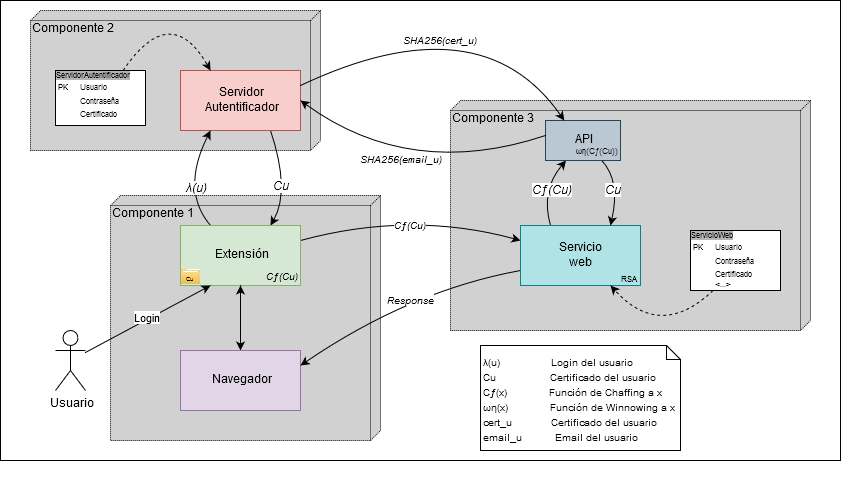
\includegraphics[width=15cm]{./imagenes/Analisis/ArquitecturaSistema.png}
        		\caption{Arquitectura General del Sistema}
	            \end{center}
	        \end{figure}    
	        \subsection{Descripci\'on de la arquitectura del sistema.}
	            El sistema se compone de 3 grandes bloques los cuales se comunicar\'an v\'ia red:
	            \begin{enumerate}
	                \item \textbf{Navegador Chrome con la Extensi\'on instalada}: Este primer bloque es el que se encuentra interactuando directamente con el usuario de nuestro sistema, consiste en la extensión creada por nosotros y el navegador en el que el usuario realiza peticiones a diferentes servicios en la web.
	                \item \textbf{Servidor autentificador:} Este bloque va ser el encargado de generar los certificados para cada usuario que se registre en la extensión y enviarlos a la extensión. Para la generación de dichos certificados utilizaremos una autoridad certificadora con lo que garantizamos la seguridad de estos mismos. Por otro lado para almacenar los datos de nuestros usuarios contaremos con una tabla que contenga como principales campos:
	                    \begin{itemize}
	                        \item Usuario
	                        \item Contraseña
	                        \item Certificado
	                    \end{itemize}
	                \item \textbf{Servidor web con API instalada: }En este módulo el servicio web contar\'a con una API, que se encargará de reconocer las peticiones que se reciban con nuestro método de autenticación y ser\'a la encargada de interpretar los datos y facilitarle la informaci\'on de autenticaci\'on al servicio.
	                Es importante destacar que el servicio almacenar\'a el certificado en cuesti\'on para que el usuario pueda autenticarse la próxima vez de forma automática.
	            \end{enumerate}
	        
	        Es importante mencionar que la comunicaci\'on entre cada uno de los bloques se realizar\'a mediante t\'ecnicas que permitan la confidencialidad de los datos, por un lado la comunicación del certificado que viajará entre la extensión y el servicio web se encontrará oculto mediante Chaffing and Winnowing y el patr\'on necesario para el m\'etodo se encontrar\'a cifrado mediante RSA. La comunicación entre el Servidor autentificador y la Extensión se encontrar\'a oculto mediante un socket seguro. 
    	
    	%%%%%%%%%%%%%%%%%%%%%%%%%%%%%%%%%%%%%%%%%%%%%%%%%%%%%%%%%
		%                                                       %
		%                                                       %
		%                       DCU General                     %
		%                                                       %
		%                                                       %
		%%%%%%%%%%%%%%%%%%%%%%%%%%%%%%%%%%%%%%%%%%%%%%%%%%%%%%%%%
	    \section{Diagrama de casos de uso general.}
	         \begin{figure}[H]
        		\begin{center}
        		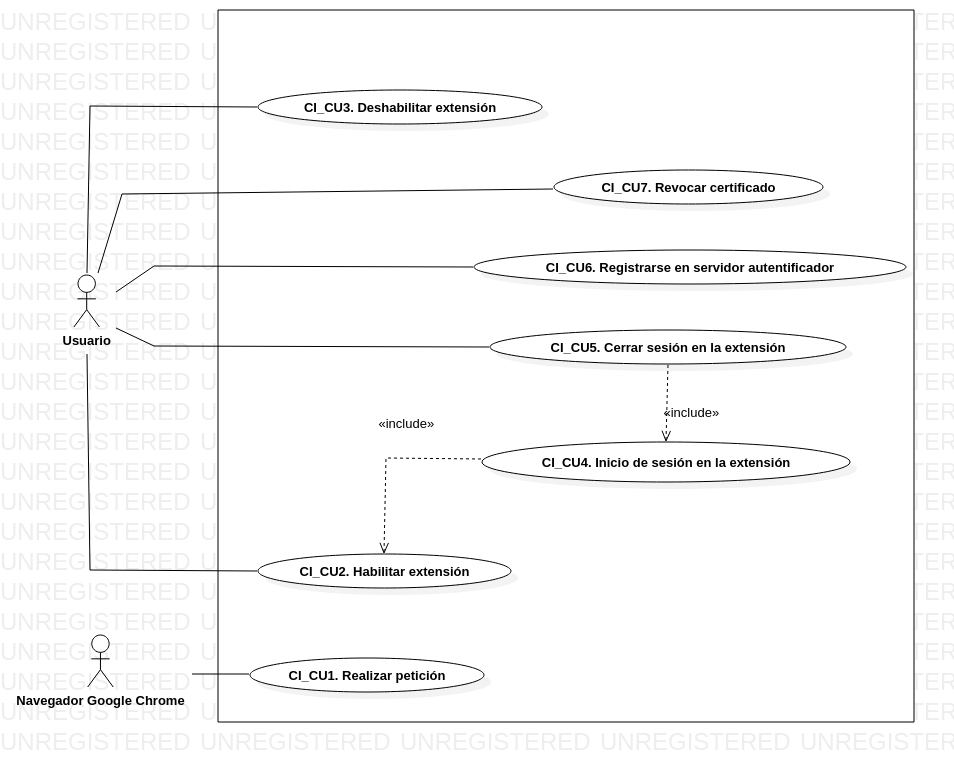
\includegraphics[width=13cm]{./imagenes/Analisis/UCD_General.png}
        		\caption{Diagrama de casos de uso general del sistema}
	            \end{center}
	        \end{figure}   
	        
	        NOTA: En la sección diseño, cada prototipo describirá sus casos de uso correspondientes para su funcionamiento.
	
		
		%%%%%%%%%%%%%%%%%%%%%%%%%%%%%%%%%%%%%%%%%%%%%%%%%%%%%%%%%
		%                                                       %
		%                                                       %
		%                      Análisis PI                     %
		%                                                       %
		%                                                       %
		%%%%%%%%%%%%%%%%%%%%%%%%%%%%%%%%%%%%%%%%%%%%%%%%%%%%%%%%%
    
		\section{Componente I. Extensión.}
		    \subsection{Descripción.}
		    
		    Este prototipo permite a la extensión poder interceptar peticiones hechas por el usuario a través del navegador de Google Chrome, una vez que se intercepte la petición, ésta podrá ser modificada. La modificación se hará sólo mientras la extensión esté habilitada, y tiene como objetivo inyectar el certificado autentificador en el encabezado del protocolo. Este certificado será simulado (sólo para este prototipo) por la misma extensión a partir de los datos del inicio de sesión. Para la creación de dicho certificado, se usará el algoritmo de hashing SHA-1, tomando como argumentos de entrada usuario y contraseña, generando así, una cadena resultante de 160 bits, sin embargo, para los siguientes prototipos, se manejará una autoridad certificadora la cual recibirá los datos del inicio de sesión para que genere el certificado del usuario. Una vez que dicho certificado es inyectado, la extensión deberá liberar la petición para que salga a red.\\
		    
		    El propósito de este prototipo es utilizar la técnica de \textit{Chaffing and Winnowing} en este nuevo método de autentificación, para evitarle al usuario la tediosa tarea de ingresar sus credenciales cada vez que accede al servicio y brindarle la seguridad necesaria al iniciar de sesión.\\
		    
		    Para inyectar el certificado autentificador, es necesario crear un \textit{''patrón de chaffing''}, este patrón lo generaremos aleatoriamente para después mandarlo junto con la petición HTTP. Por el momento, dicho patrón no irá cifrado, ya que para esto es necesario la implementación del servidor del servicio web de prueba, para poder conocer su llave pública y cifrar el patrón. Sin embargo, en el prototipo 1 del subsistema 3 se implementará el servidor y con ello su cifrado asimétrico. El objetivo de mandar el patrón junto con el protocolo HTTP, es que el servidor pueda leer el patrón y realizar la etapa de \textit{winnowing}, para extraer el certificado.\\
            
          
				\begin{comment}
				\paragraph{API FileSystem \\}
				Consiste en una API muy útil para trabajar con archivos en el entorno de desarrollo de Google Chrome, soporta la entrada de archivos y directorios desde una computadora personal. La ventaja de esta API es que no es necesario acceder a todos los archivos del usuario, si no que se crea una especie de unidad virtual en donde se localizan los archivos que el usuario deseé utilizar, en este caso en la extensión \cite{filesystemmozilla}.
				
				%\paragraph {hay que usar otra madre pero no se que alv. \\}
				\paragraph{OpenSSL}
				SSL (Secure Sockets Layer o capa de conexión segura) es un estándar de seguridad global que permite la transferencia de datos cifrados entre un navegador y un servidor web. Es utilizado por millones \cite{opensslmillones} de empresas e individuos en línea a fin de disminuir el riesgo de robo y manipulación de información confidencial (como números de tarjetas de crédito, nombres de usuario, contraseñas, correos electrónicos, etc.) por parte de hackers y ladrones de identidades. Básicamente, la capa SSL permite que dos partes tengan una "conversación" privada.
				Para establecer esta conexión segura, se instala en un servidor web un certificado SSL (también llamado "certificado digital") que cumple dos funciones: Autenticar la identidad del sitio web, garantizando a los visitantes que no están en un sitio falso y cifrar la información transmitida.
				Openssl es una api que proporciona un entorno adecuado para encriptar los datos enviados a otra computadora dentro de una red y a su vez desencriptarlos adecuadamente por el receptor, evitando así, el acceso a la información por intrusos con la utilización de sniffer.
				El conjunto de herramientas OpenSSL es una característica de FreeBSD que ofrece una capa cifrada de transporte sobre la capa normal de comunicación, permitiendo la combinación con muchas aplicaciones y servicios de red. 
                Uno de los usos más comunes de OpenSSL es ofrecer certificados para usar con aplicaciones de software. Estos certificados aseguran que las credenciales de la compañía o individuo son válidos y no son fraudulentos. Si el certificado en cuestión no ha sido verificado por uno de las diversas “autoridades certificadoras” o CA, suele generarse una advertencia al respecto. Una autoridad de certificados es una compañía, que firma certificados para validar credenciales de individuos o compañías. Este proceso tiene un costo asociado y no es un requisito imprescindible para usar certificados, aunque puede darle un poco de tranquilidad a los usuarios \cite{openssl}.
                %filesystemmozilla https://developer.mozilla.org/es/docs/Web/API/FileSystem
				% opensslmillones https://www.verisign.com/es_LA/website-presence/online/ssl-certificates/index.xhtml
				%openssl https://www.globalsign.com/es/centro-de-informacion-ssl/que-es-ssl/
				\end{comment}
			
			%%%%%%%%%%%%%%%%%%%%%%%%%%%%%%%%%%%%%%%%%%%%%%%%%%%%%%%%%
			%                                                       %
			%                                                       %
			%                REQUERIMIENTOS PII                     %
			%                                                       %
			%                                                       %
			%%%%%%%%%%%%%%%%%%%%%%%%%%%%%%%%%%%%%%%%%%%%%%%%%%%%%%%%%
			
		    \subsection{Estudio de requerimientos.}
				\subsubsection{Requerimientos Funcionales.}
				{\setlength{\parindent}{12pt}
				
				\textbf{CI\_RF1. Interceptar petición \acrshort{http}.} La extensión deberá interceptar la petición \acrshort{http} del navegador, en cuanto el usuario realice alguna a través de éste.\\

				\textbf{CI\_RF2. Deshabilitar extensión.} El usuario podrá deshabilitar la extensión, para que ésta no vigile su actividad en el navegador.\\
				
				\textbf{CI\_RF3. Habilitar extensión.} El usuario podrá habilitar la extensión, para que ésta vigile las peticiones \acrshort{http}.\\
				
				\textbf{CI\_RF4. Validar petición.} La extensión deberá analizar la petición previamente recibida, y validar si ésta es HTTP(S) o no.\\
				
				\textbf{CI\_RF5. Bloquear salida de petición.} La extensión deberá evitar que la petición salga a red, deteniéndola para aplicar la etapa de \textit{Chaffing}.\\ 
				
				\textbf{CI\_RF6. Inicio de sesi\'on en la extensi\'on.} La extensi\'on contar\'a con una interfaz para el ingreso de datos del usuario, donde ingresará un usuario y contraseña. \\  
				
                \textbf{CI\_RF7. Generación del certificado autentificador.} Para este prototipo, la generación del certificado autentificador se har\'a del lado del cliente, simulando la tarea de una entidad certificadora, permitiendo as\'i generar automáticamente esta llave la cual servir\'a para el proceso de \textit{chaffing} del mensaje en el protocolo HTTP.\\
                
                \textbf{CI\_RF8. Almacenamiento del certificado autentificador.} La extensi\'on deberá almacenar el certificado autentificador.\\
                
                \textbf{CI\_RF9. Generación de patrón de \textit{Chaffing}.} La extensión generará un patrón para poder implementar el método de \textit{Chaffing}. Este patrón será generado al azar, y es aquel que se usará para introducir el código autentificador en el protocolo HTTP.\\
                
				\textbf{CI\_RF10. Etapa de \textit{Chaffing}.} Por medio del m\'etodo \textit{Chaffing} se crearán paquetes para agregar al encabezado HTTP que se ha interceptado gracias al requerimiento funcional CI\_RF1. Interceptar petición HTTP, utilizando el patrón de \textit{Chaffing} del requerimiento funcional CI\_RF9. Generación de patrón de \textit{Chaffing}\\
                    
                \textbf{CI\_RF11. Liberaci\'on de Petición.} Se liberar\'a el bloqueo a la petici\'on HTTP impuesto por el requerimiento funcional CI\_RF5. Bloquear salida de petición.
                
		        }
				
				\subsubsection{Requerimientos no Funcionales.}
				{\setlength{\parindent}{12pt}
				
				\textbf{CI\_RNF1. Plataforma de implementación.} La extensión será implementada en el navegador Google Chrome Desktop.\\
				
				\textbf{CI\_RNF2. Versión del navegador} La extensión funcionará a partir de la versión 28.0.\\
				
				\textbf{CI\_RNF3. Tecnologías para la interfaz de usuario} Para el sistema se hará uso de HTML5, JavaScript, CSS3, JSON.\\
				
				\textbf{CI\_RNF4. Permitir ejecución de JavaScript en Google Chrome.} Para el correcto funcionamiento de la extensión, es necesario que se permita la ejecución de javascript en el navegador Google Chrome.\\
				
				\textbf{CI\_RNF5. Conexión a internet.} Para el funcionamiento de la extensión, no es necesario que se tenga conexión a internet.\\
				
				\textbf{CI\_RNF6. Tamaño del código autentificador.} El tamaño del código autentificador es de 160 bits. Para este prototipo se hará uso de la función \textit{hash} tomando como argumentos el nombre de usuario y contraseña del usuario que se desea generar el código de hash.\\
				
				\textbf{CI\_RNF7. Almacenado de archivo en la extensión.} Se necesita tener almacenado el archivo en la extensión de Google Chrome. Específicamente, utilizamos el \textbf{Storage} para almacenarlo. \\
				
				\textbf{CI\_RNF8. Conexión a internet.} Para el funcionamiento de este prototipo, es necesario tener acceso a internet. \\
				}
		    
		    \subsection{Reglas del negocio.}
		    %Martin y Odell (1998) y Russel (1995) proponen que una regla de negocio es un restricción que opera sobre el sistema.
		    
		    \textbf{CI\_RN1. Extensión habilitada.} En cuanto el usuario lo indique por medio de la \acrlong{iu}, la extensión deberá vigilar la actividad que éste realice en el navegador para interceptar una petición.\\
			\label{CI_RN1}
			
			\textbf{CI\_RN2. Extensión deshabilitada.} En cuanto el usuario lo indique por medio de la \acrlong{iu}, la extensión deberá dejar de vigilar la actividad que éste realice en el navegador.\\
			\label{CI_RN2}
			
            \textbf{CI\_RN3. Petición válida.} La extensión modificará la petición siempre y cuando se trate de una petición válida HTTP .\\
            \label{CI_RN3}
            
            \textbf{CI\_RN4. Inicio de sesión de extensión por usuario.} Cada usuario que desee utilizar la extensión sólo deberá tener una cuenta con un usuario y una contraseña respectiva a este usuario. \\
            \label{CI_RN4}
            
            \textbf{CI\_RN5. Acceso a internet.} Se debe de contar con acceso a internet para que la extensión pueda enviar al servidor la petición modificada.\\
            \label{CI_RN5}
				
			\textbf{CI\_RN6. Longitud de código autentificador.} La longitud del código autentificador es de 40 caracteres, debido a que la función de SHA-1 es un algoritmo de codificación de 160 bits que genera un hash hexadecimal de 40 caracteres.\\
			\label{CI_RN6}
			
			\textbf{CI\_RN7. Longitud del campo de usuario.} La longitud del usuario no debe pasar de 20 caracteres, y mínimo será de 3 caracteres.\\
			\label{CI_RN7}
			
			\textbf{CI\_RN8. Longitud del campo contraseña.}
			La longitud de la contraseña no debe pasar de 16 caracteres, y mínimo sera de 8 caracteres.\\
			\label{CI_RN8}
			
			\textbf{CI\_RN9. Caracteres permitidos en campo usuario.} Los caracteres permitidos en el campo de usuario son unicamente símbolos alfanúmericos y guion bajo.\\
			\label{CI_RN9}
			
			\textbf{CI\_RN10. Caracteres permitidos en campo contraseña.} Los caracteres permitidos en el campo de contraseña son unicamente símbolos alfanúmericos así como los s\'imbolos \_ @ / \# ? .\\
			\label{CI_RN10}
			
			\textbf{CI\_RN11. Formato de contraseña.} La contraseña debe tener al menos un número y una letra mayúscula.\\
			\label{CI_RN11}
				
	    %%%%%%%%%%%%%%%%%%%%%%%%%%%%%%%%%%%%%%%%%%%%%%%%%%%%%%%%%
		%                                                       %
		%                                                       %
		%       Análisis CII: SERVIDOR AUTENTIFICADOR           %
		%                                                       %
		%                                                       %
		%%%%%%%%%%%%%%%%%%%%%%%%%%%%%%%%%%%%%%%%%%%%%%%%%%%%%%%%%
	        
	   \section{Componente II: Servidor autentificador.}
	        \subsection{Descripción.}
	        Para este componente, vamos a implementar un servidor autentificador en el cual se crearán y almacenarán los certificados de los usuarios en una base de datos. En este servicio, los usuarios tendrán registrada una cuenta a la cual accederán desde la extensión del componente 1. Una vez que inicien sesión en la extensión, este servidor autentificador regresará como respuesta el certificado generado para que la extensión lo almacene. Para la creación del certificado autentificador se utilizará la herramienta OpenSSL, además, la comunicación entre extensión y servidor se hará bajo SSL/TLS.\\
	        
	        La principal función de este componente es gestionar las cuentas y certificados en una base de datos, de tal forma que el componente 1 (extensión de Google Chrome) se pueda comunicar con este componente ya sea para que le genere un certificado a una cuenta (en el caso de que el usuario se esté registrando en el servidor autentificador por primera vez) o para mandarle su certificado si es que ya se encuentra registrado en el servidor.\\
	        
	        El propósito de este componente es poder crear y utilizar un certificado real, generado por una autoridad certificadora de confianza y con el cual se pueda autentificar a un usuario en un servicio web. Como sabemos, el certificado emitido por la autoridad certificadora es de tipo público por lo que puede ser visible para cualquier entidad.\\
	       
	        \subsection{Estudio de requerimientos.}
	            \subsubsection{Requerimientos funcionales.}
	            {\setlength{\parindent}{12pt}
				
				\textbf{CII\_RF1. Creación de nuevo usuario.} La autoridad certificadora podrá crear una nueva instancia en la base de datos de acuerdo a los datos recuperados por la extensión (Usuario y contraseña), si es que estos no se encuentran guardados en la base de datos.\\

				\textbf{CII\_RF2. Generar certificado.} La autoridad certificadora deberá generar un certificado diferente para cada usuario que se registre en la extensión con los datos proporcionados por la misma.\\
				
				\textbf{CII\_RF3. Asignar certificado.} La autoridad certificadora deberá asignar el certificado generado al usuario correspondiente en la base de datos.\\
				
				\textbf{CII\_RF4. Devolver certificado.} La autoridad certificadora deberá enviar el certificado correspondiente al usuario quien realiza la solicitud para obtener el certificado.\\
				
				\textbf{CII\_RF5. Actualizar certificado.} La autoridad certificadora deberá actualizar el certificado cuanto éste haya caducado.
                
		        }
		        
	            \subsubsection{Requerimientos no funcionales.}
	            {\setlength{\parindent}{12pt}
				
				\textbf{CII\_RNF1. Plataforma de implementación.} La autoridad certificadora será implementada en NodeJs.\\
				
				\textbf{CII\_RNF2. Version de SSL/TLS.} La autoridad certificadora usará como conexión, así como la generación de certificado, OpenSSL con la versión 1.1.1.\\
				
				\textbf{CII\_RNF3. Base de datos.} La autoridad certificadora se conectará a una base de datos MongoDB 4.0.10.\\
				
				}
	            
	            
	        \subsection{Reglas del negocio.}
	        
	        \textbf{CII\_RN1. Acceso a internet.} Se debe de contar con acceso a internet para que la autoridad certificadora pueda enviar a la extensión el certificado generado.\\
            \label{CII_RN1}
            
            \textbf{CII\_RN2. Conexión a la base de datos.} La autoridad certificadora cuenta con un pull de conexiones a la base de datos para poder insertar u obtener certificados de los usuarios.\\
            \label{CII_RN2}
            
            \textbf{CII\_RN3. Conexión SSL.} La autoridad certificadora tiene una conexión SSL con la extensión para poder así enviar el certificado de manera segura y cifrada.\\
            \label{CII_RN3}
			
			%%%%%%%%%%%%%%%%%%%%%%%%%%%%%%%%%%%%%%%%%%%%%%%%%%%%%%%%%
    		%                                                       %
    		%                                                       %
    		%            Análisis CIII: SERVICIO WEB                %
    		%                                                       %
    		%                                                       %
    		%%%%%%%%%%%%%%%%%%%%%%%%%%%%%%%%%%%%%%%%%%%%%%%%%%%%%%%%%
	       
	       \section{Componente III: Servicio Web y API.}
	        \subsection{Descripción.}
	        Para el componente III, se va a implementar un servicio web de prueba para realizar la etapa de \textit{winnowing} a la petición HTTP que reciba de la extensión. Esto implica la modificación del servidor de prueba implementado en Apache para que detecte este tipo de autentificación y la creación de un algoritmo que realice el procesos de \textit{winnowing} al protocolo. 
	        Así mismo, el servicio web implementará un cifrado asimétrico (RSA), esto con la finalidad de que el componente I pueda tomar la llave pública del servidor y cifrar el \textit{''patrón de chaffing''} que se mandará en la petición. Este servidor web tendrá una API la cuál se encargará de realizar el proceso de \textit{winnowing}, descifrando lo que reciba del componente I con la llave privada del servidor.\\
            
            El propósito de este componente es poder obtener el certificado que identificará a cada usuario, para poder validarlo y saber si se debe de dar acceso o negar el mismo. Cabe mencionar que, la primera vez que el servidor reciba el certificado autentificador en cada servicio, pedirá al usuario que se inicie sesión con la finalidad de poder asociar este certificado a una cuenta de un servicio; para las peticiones posteriores, el certificado ya contará con una cuenta asociada a la cual podrá dar acceso siempre y cuando las credenciales sean correctas.\\
            
	        \subsection{Estudio de requerimientos.}
	            \subsubsection{Requerimientos funcionales.}
	            \textbf{CIII\_RF1. Guardar certificados.} Si el servidor no tiene asociado el certificado que se recibe del componente I en la base de datos, éste lo guardará asociandolo con un inicio de sesión.\\
	            
	            \textbf{CIII\_RF2. Comunicación con autoridad certificadora.} El servidor autentificador podrá tener comunicación con una autoridad certificadora para el intercambio de información.\\
	                
	            \textbf{CIII\_RF3. Obtención de certificado autentificador.} Una vez realizada la comunicación con la autoridad certificadora, obtendremos un certificado auntentificador que identificará a un usuario.\\
	            
	            %\textbf{CIII\_RF4. Eliminar certificado autentificador.} El servidor web podrá eliminar un certificado asociado a una cuenta.\\ 
	            
	            \textbf{CIII\_RF4. Generación de llaves.} El servidor web puede generar un par de llaves (pública y privada) para su uso en cifrados asimétricos (en este caso, RSA).\\
	       
	            \subsubsection{Requerimientos no funcionales.}
	                \textbf{CIII\_RNF1. Plataforma de implementación.} Las pruebas del servidor web serán realizadas en el servidor Apache2.\\

	                \textbf{CIII\_RNF2. Base de datos.} Se utilizará una base de datos en MySQL para guardar la información de los usuarios.\\
	                
	                \textbf{CIII\_RNF3. Tamaño de llaves.} Se utilizarán llaves de un tamaño de 2048 bits para el cifrado de tipo RSA.\\
	                
	       
	            \subsubsection{Reglas del negocio.}
    	            \textbf{CIII\_RN1. Conexión a internet.} Se debe de contar con una conexión estable a internet para evitar perder paquetes en todo el proceso.\\
    	            
    	            \textbf{CIII\_RN2. Conexión a base de datos.} El servidor debe tener una correcta conexión a la base de datos para su correcto funcionamiento.\\
    	            
    	            \textbf{CIII\_RN3. API en el servidor.} El servidor debe de contar con la API para que pueda realizar el procesos de \textit{winnowing}.
	
	
	%%% http://www.math.com.mx/longitud%20de%20claves.html
	
	
	
	
	
	%%%%%%%%%%%%%%%%%%%%%%%%%%%%%%%%%%%%%%%%%%%%%%%%%%%%%%%%%
	%                                                       %
	%                                                       %
	%                      Desarrollo                       %
	%                                                       %
	%                                                       %
	%%%%%%%%%%%%%%%%%%%%%%%%%%%%%%%%%%%%%%%%%%%%%%%%%%%%%%%%% 
	    
	\chapter{\textcolor{azulescom}{Diseño.}}
			
		\section{Componente I.}
		 
		    \subsection{Diagrama de casos de uso}
			    
			    \begin{figure}[H]
		            \begin{center}			                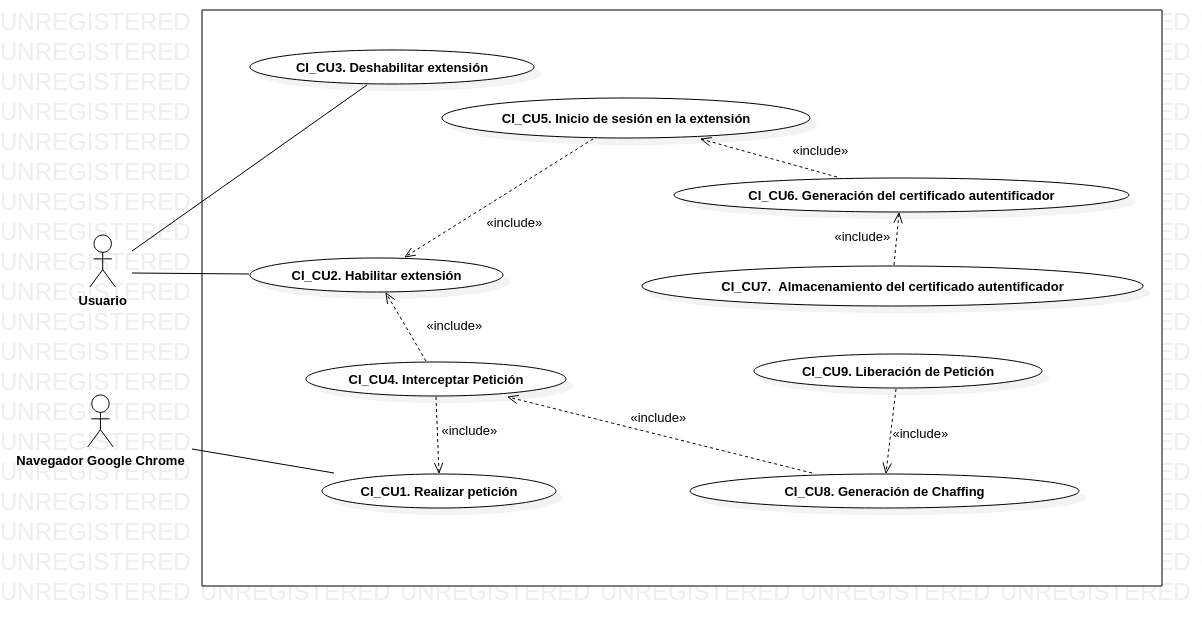
\includegraphics[width=16cm]{./imagenes/Disenio/Componente_1/CI_UCD_P1.png}
						\caption{Diagrama de casos de uso del Componente I.}
                    \end{center}    					
				\end{figure}
			    
	        \subsection{Descripción de casos de uso.}
			    
			    %%Descripcion PI_CU1
			    \begin{table}[H]
				\begin{tabular}{ |p{3.5cm}||p{9.5cm}|}
					\hline
					\rowcolor{guindapoli}
					\multicolumn{2}{|c|}{\textbf{\textcolor{white}{Caso de uso: CI\_CU1. Realizar petición.}}}\\
					\hline
					\rowcolor{azulfuerte}Concepto & Descripción\\
					\hline
					\cellcolor{azulclaro}Actor & 
					Navegador de Google Chrome.\\ 
					\hline
					\cellcolor{azulclaro}Propósito &
					Este caso de uso permite al navegador realizar una petición \acrshort{http}, ordenada por el usuario o un sistema externo.\\
					\hline
					\cellcolor{azulclaro}Entradas &
					URL del servicio web solicitado.\\
					\hline
					\cellcolor{azulclaro}Salidas &
					Petición \acrshort{http}.\\
					\hline
					\cellcolor{azulclaro}Pre-condiciones&
					Algún agente externo (Sistema o usuario) ha ordenado al navegador mandar una petición \acrshort{http}.\\
					\hline
					\cellcolor{azulclaro}Post-condiciones&
					Creación de la petición HTTP.\\
					\hline
					\cellcolor{azulclaro}Reglas del negocio&
					-\\
					\hline
					\cellcolor{azulclaro}Errores &
					La petición no se pudo realizar. \newline La petición no es tipo \acrshort{http}.\\					
					\hline
				\end{tabular}
				\caption[DCU: CI\_CU1]{Descripción CU: CI\_CU1}
				\end{table}
				
				\paragraph{... Trayectoria Principal ...}
				\begin{enumerate}
					\item \textbf{\textit{El Usuario}} o \textbf{\textit{El Sistema Externo}} realiza una petición \acrshort{http} en el navegador Google Chrome.\\
					\item \textbf{\textit{El navegador}} realiza la petición.\\
				\end{enumerate}
				\paragraph{... Fin de la Trayectoria Principal ...}
				
				\paragraph{... Trayectoria Alternativa 1 ...}
				\begin{enumerate}
					\item \textbf{\textit{El Usuario}} o \textbf{\textit{El Sistema Externo}} realiza una petición que no es \acrshort{http} en el navegador Google Chrome.\\
					\item \textbf{\textit{El navegador}} realiza la petición.					
				\end{enumerate}
				\paragraph{... Fin de la Trayectoria Alternativa 1 ...}
				
				%%Descripcion PI_CU2
				\begin{table}[H]
				\begin{center}
				\begin{tabular}{ |p{3.5cm}||p{9.5cm}|}
					\hline
					\rowcolor{guindapoli}
					\multicolumn{2}{|c|}{\textbf{\textcolor{white}{Caso de uso: CI\_CU2. Habilitar extensión.}}}\\
					\hline
					\rowcolor{azulfuerte}Concepto & Descripción\\
					\hline
					\cellcolor{azulclaro}Actor & 
					Usuario.\\ 
					\hline
					\cellcolor{azulclaro}Propósito &
					Este caso de uso, permite al usuario habilitar la extensión, para que ésta sea capaz de ver todas las peticiones que realiza el navegador.\\
					\hline
					\cellcolor{azulclaro}Entradas &
					Indicación de habilitar extensión, mediante interfaz de usuario.\\
					\hline
					\cellcolor{azulclaro}Salidas &
					-\\
					\hline
					\cellcolor{azulclaro}Pre-condiciones&
					{\textbf{CI\_CU3.}}\\
					\hline
					\cellcolor{azulclaro}Post-condiciones&
					-\\
					\hline
					\cellcolor{azulclaro}Reglas del negocio&
					\hyperref[CI_RN1]{\textbf{CI\_RN1.}}\\
					\hline
					\cellcolor{azulclaro}Errores &
					No se puede habiliar la extensión.\\
					\hline
				\end{tabular}
				\caption[DCU: CI\_CU2]{Descripción CU: CI\_CU2}
				\end{center}
				\end{table}
				
				\paragraph{... Trayectoria Principal ...}
				\begin{enumerate}
					\item \textbf{\textit{El usuario}} da click en el ícono de la extensión \img{imagenes/Disenio/Componente_1/escom.png}.
					\item \textbf{\textit{El usuario}} da click en el botón \img{imagenes/Disenio/Componente_1/boton_activar.png}.
					\item \textbf{\textit{La extensión}} empieza a vigilar las peticiones que se realicen a través del navegador.
				\end{enumerate}
				\paragraph{... Fin de la Trayectoria Principal ...}
				
				\paragraph{... Trayectoria Alternativa 1 ...}
				\begin{enumerate}
				    \item \textbf{\textit{La extensión}} no muestra el botón \img{imagenes/Disenio/Componente_1/boton_activar.png}, por ende el usuario no puede dar click.
				\end{enumerate}
				\paragraph{... Fin de la Trayectoria Alternativa 1 ...}
				
				%%Descricpion PI_CU3
				\begin{table}[H]
				\begin{center}
				\begin{tabular}{ |p{3.5cm}||p{9.5cm}|}
					\hline
					\rowcolor{guindapoli}
					\multicolumn{2}{|c|}{\textbf{\textcolor{white}{Caso de uso: CI\_CU3. Deshabilitar extensión.}}}\\
					\hline
					\rowcolor{azulfuerte}Concepto & Descripción\\
					\hline
					\cellcolor{azulclaro}Actor & 
					Usuario.\\ 
					\hline
					\cellcolor{azulclaro}Propósito &
					Este caso de uso permite al usuario deshabilitar la extensión, para que ésta ignore todas las peticiones que se realicen por medio del navegador.\\
					\hline
					\cellcolor{azulclaro}Entradas &
					Indicación de deshabilitar extensión, mediante interfaz de usuario.\\
					\hline
					\cellcolor{azulclaro}Salidas &
					-\\
					\hline
					\cellcolor{azulclaro}Pre-condiciones&
				    {\textbf{CI\_CU2.}}\\
					\hline
					\cellcolor{azulclaro}Post-condiciones&	-\\
					\hline
					\cellcolor{azulclaro}Reglas del negocio&
					\hyperref[CI_RN2]{\textbf{CI\_RN2.}}\\
					\hline
					\cellcolor{azulclaro}Errores &
					No se puede deshabilitar la extensión.\\
					\hline
				\end{tabular}
				\caption[DCU: CI\_CU3]{Descripción CU: CI\_CU3}
				\end{center}
				\end{table}
			
				\paragraph{... Trayectoria Principal ...}
				\begin{enumerate}
					\item \textbf{\textit{El usuario}} da click en el ícono de la extensión \img{imagenes/Disenio/Componente_1/escom.png}.
					\item \textbf{\textit{El usuario}} da click en el botón \img{imagenes/Disenio/Componente_1/boton_desactivar.png}.
					\item \textbf{\textit{La extensión}} deja de vigilar las peticiones que se realicen a través del navegador.
				\end{enumerate}
				\paragraph{... Fin de la Trayectoria Principal ...}
				
		        \paragraph{... Trayectoria Alternativa 1 ...}
				\begin{enumerate}
				     \item \textbf{\textit{La extensión}} no muestra el botón \img{imagenes/Disenio/Componente_1/boton_desactivar.png}, por ende el usuario no puede dar click.
				\end{enumerate}
				\paragraph{... Fin de la Trayectoria Alternativa 1 ...}
				
				%%Descricpion PI_CU4
				\begin{table}[H]
				\begin{center}
				\begin{tabular}{ |p{3.5cm}||p{9.5cm}|}
					\hline
					\rowcolor{guindapoli}
					\multicolumn{2}{|c|}{\textbf{\textcolor{white}{Caso de uso: CI\_CU4. Interceptar petición.}}}\\
					\hline
					\rowcolor{azulfuerte}Concepto & Descripción\\
					\hline
					\cellcolor{azulclaro}Actor & 
					 -.\\ 
					\hline
					\cellcolor{azulclaro}Propósito &
					Este caso de uso interceptará las peticiones HTTP que el navegador realice para su analisis.\\
					\hline
					\cellcolor{azulclaro}Entradas &
					Petición realizada por el navegador\\
					\hline
					\cellcolor{azulclaro}Salidas &
					-\\
					\hline
					\cellcolor{azulclaro}Pre-condiciones&
				    \textbf{CI\_CU1.} \newline \textbf{CI\_CU2.}\\
					\hline
					\cellcolor{azulclaro}Post-condiciones&-\\
					\hline
					\cellcolor{azulclaro}Reglas del negocio&
					\hyperref[CI_RN1]{\textbf{CI\_RN1.}} \newline
					\hyperref[CI_RN3]{\textbf{CI\_RN3.}}\\
					\hline
					\cellcolor{azulclaro}Errores &
					La petición no se genera correctamente.\\
					\hline
				\end{tabular}
				\caption[DCU: CI\_CU4]{Descripción CU: CI\_CU4}
				\end{center}
				\end{table}
			    \label{PI_CU4}
				\paragraph{... Trayectoria Principal ...}
				\begin{enumerate}
					\item \textbf{\textit{El usuario}} ingresa una URL en el navegador. 
					\item \textbf{\textit{El navegador}} genera una petición HTTP. 
					\item \textbf{\textit{La extensión}} Intercepta la petición realizada por el navegador para su análisis
				\end{enumerate}
				\paragraph{... Fin de la Trayectoria Principal ...}
			    
				%%DESCRIPCIÓN PI_CU5
				\begin{table}[H]
    				\begin{tabular}{ |p{3.5cm}||p{9.5cm}|}
    					\hline
    					\rowcolor{guindapoli}
    					\multicolumn{2}{|c|}{\textbf{\textcolor{white}{Caso de uso: CI\_CU5. Inicio de sesión en la extensión}}}\\
    					\hline
    					\rowcolor{azulfuerte}Concepto & Descripción\\
    					\hline
    					\cellcolor{azulclaro}Actor & 
    					Usuario\\ 
    					\hline
    					\cellcolor{azulclaro}Propósito &
    					Este caso de uso permite al usuario poder iniciar sesión en la extensión para posteriormente obtener un código autentificador, basado en esos datos, al cual se le aplicará \textit{Chaffing}. \newline
    					Sólo se requerirá iniciar sesión una sola vez, ya que después, sólo es necesario CIr el código generado para autentificarse en el servicio web.\\
    					\hline
    					\cellcolor{azulclaro}Entradas &
    					Usuario y Contraseña\\
    					\hline
    					\cellcolor{azulclaro}Salidas &
    					Código autentificador el cual hace referencia al usuario iniciado\\
    					\hline
    					\cellcolor{azulclaro}Pre-condiciones&
    					Haber instalado la extensión en el navegador Google Chrome y habiéndola habilitado.\\
    					\hline
    					\cellcolor{azulclaro}Post-condiciones&
    					Con los datos introducidos por el usuario, se obtendrá el código autentificador del mismo, para que lo guarde en su dispositivo y lo pueda usar después.\\
    					\hline
    					\cellcolor{azulclaro}Reglas del negocio&
    					\hyperref[CI_RN2]{\textbf{CI\_RN1.}} \newline \hyperref[CI_RN3]{\textbf{CI\_RN4.}} \newline
    					\hyperref[CI_RN6]{\textbf{CI\_RN7.}} \newline
    					\hyperref[CI_RN7]{\textbf{CI\_RN8.}} \newline
    					\hyperref[CI_RN8]{\textbf{CI\_RN9.}} \newline
    					\hyperref[CI_RN9]{\textbf{CI\_RN10.}} \newline
    					\hyperref[CI_RN10]{\textbf{CI\_RN11.}} \\
    					\hline
    					\cellcolor{azulclaro}Errores &
    					No se encuentra usuario registrado \newline 
    					No se puede obtener el código autentificador\newline
    					No se pudo guardar el código autentificador\newline
    					Contraseña no válida\\					
    					\hline
    				\end{tabular}
				\caption[DCU: CI\_CU5]{Descripción CU: CI\_CU5}
				\end{table}
				
				\paragraph{... Trayectoria Principal ...}
				\begin{enumerate}
					\item \textbf{\textit{El Usuario}} realiza un inicio de sesión por primera vez en la extensión.
					\item \textbf{\textit{La extensión}} obtendrá los parametros de usuario y contraseña para generar un código autentificador único.
				\end{enumerate}
				\paragraph{... Fin de la Trayectoria Principal ...}
				
				\paragraph{... Trayectoria Alternativa 1 ...}
				\begin{enumerate}
					\item \textbf{\textit{El Usuario}} ingresa usuario y/o contraseña no validos.
					\item \textbf{\textit{La extensión}} no podrá obtener los datos del usuario.
				\end{enumerate}
				\paragraph{... Fin de la Trayectoria Alternativa 1 ...}
				
				\newpage
				
				%%DESCRIPCIÓN PI_CU6
				\begin{table}[H]
    				\begin{tabular}{ |p{3.5cm}||p{9.5cm}|}
    					\hline
    					\rowcolor{guindapoli}
    					\multicolumn{2}{|c|}{\textbf{\textcolor{white}{Caso de uso: CI\_CU6. Generación del certificado autentificador.}}}\\
    					\hline
    					\rowcolor{azulfuerte}Concepto & Descripción\\
    					\hline
    					\cellcolor{azulclaro}Actor & 
    					 -\\ 
    					\hline
    					\cellcolor{azulclaro}Propósito &
    					Este caso de uso generará un certificado para el usuario, basados en los datos que ingrese en la extensión (usuario y contraseña).\\
    					\hline
    					\cellcolor{azulclaro}Entradas &
    					Usuario y contraseña ingresados en la extensión.\\
    					\hline
    					\cellcolor{azulclaro}Salidas &
    					Certificado autentificador del usuario.\\
    					\hline
    					\cellcolor{azulclaro}Pre-condiciones&
    					Contar con la extensión habilitada. e ingresar un usuario y contraseña\\
    					\hline
    					\cellcolor{azulclaro}Post-condiciones&
    					 -\\
    					\hline
    					\cellcolor{azulclaro}Reglas del negocio&
    				    \hyperref[CI_RN7]{\textbf{CI\_RN7.}} \newline
    				    \hyperref[CI_RN8]{\textbf{CI\_RN8.}} \newline
    				    \hyperref[CI_RN9]{\textbf{CI\_RN9.}} \newline
    				    \hyperref[CI_RN10]{\textbf{CI\_RN10.}} \newline
    				    \hyperref[CI_RN11]{\textbf{CI\_RN11.}} \\
    					\hline
    					\cellcolor{azulclaro}Errores &
    					Error al generar el certificado.\\
    					\hline
    				\end{tabular}
				\caption[DCU: CI\_CU6]{Descripción CU: CI\_CU6}
				\end{table}
				\label{PII_CU2}
				
				\paragraph{... Trayectoria Principal ...}
				\begin{enumerate}
					\item \textbf{\textit{La extensión}} generará un código autentificador basado en los datos ingresados por el usuario.
				\end{enumerate}
				\paragraph{... Fin de la Trayectoria Principal ...}
				
				\paragraph{... Trayectoria Alternativa 1 ...}
				\begin{enumerate}
				    \item \textbf{\textit{La extensión}} no puede generar el código autentificador.
					\item \textbf{\textit{La extensión}} mostrará al usuario un mensaje de dicho error.
				\end{enumerate}
				\paragraph{... Fin de la Trayectoria Alternativa 1 ...}
				
				\newpage

				%
				%
				%       DESCRIPCIÓN PII_CU7
			    %
                %
                
				\begin{table}[H]
    				\begin{tabular}{ |p{3.5cm}||p{9.5cm}|}
    					\hline
    					\rowcolor{guindapoli}  					\multicolumn{2}{|c|}{\textbf{\textcolor{white}{Caso de uso: CI\_CU7. Almacenamiento del certificado autentificador.}}}\\
    					\hline
    					\rowcolor{azulfuerte}Concepto & Descripción\\
    					\hline
    					\cellcolor{azulclaro}Actor & 
    					-\\ 
    					\hline
    					\cellcolor{azulclaro}Propósito &
    					Este caso de uso permite que la extensión guarde el certificado autentificador, para que el usuario no tenga que hacerlo por el mismo. De esta manera, la extensión tendrá acceso al certificado cada que éste sea requerido.\newline El lugar donde se guarda dicho certificado es en ''Google Chrome Storage'', una zona de memoria que Google Chrome nos brinda al desarrollar una extensión para el navegador.\\
    					\hline
    					\cellcolor{azulclaro}Entradas &
    					Certificado autentificador.\\
    					\hline
    					\cellcolor{azulclaro}Salidas &
    					-\\
    					\hline
    					\cellcolor{azulclaro}Pre-condiciones&
    					\textbf{{CI\_CU6.}}. \\
    					\hline
    					\cellcolor{azulclaro}Post-condiciones&
    					-\\
    					\hline
    					\cellcolor{azulclaro}Reglas del negocio&
    					\hyperref[CI_RN6]{\textbf{CI\_RN6.}}\\
    					\hline
    					\cellcolor{azulclaro}Errores &
    				    No se puede almacenar el certificado autentificador.\\
    					\hline
    				\end{tabular}
				\caption[DCU: CI\_CU7]{Descripción CU: CI\_CU7}
				\end{table}
				
				\paragraph{... Trayectoria Principal ...}
				\begin{enumerate}
				    \item \textbf{\textit{La extensión}} ha creado el certificado autentificador.
				    \item \textbf{\textit{La extensión}} guarda el certificado en storage.
				    \item \textbf{\textit{La extensión}} muestra al usuario el siguiente mensaje ''Certificado guardado en Storage'' en la figura \ref{fig:UI_certSavedInStorage}
				\end{enumerate}
				\paragraph{... Fin de la Trayectoria Principal ...}
				
				\paragraph{... Trayectoria Alternativa 1 ...}
				\begin{enumerate}
				    \item \textbf{\textit{La extensión}} no ha creado el certificado autentificador.
					\item \textbf{\textit{La extensión}} no guarda el certificado autentificador en storage. 
					\item \textbf{\textit{La extensión}} muestra al usuario el siguiente mensaje ''Certificado no encontrado'' en la figura \ref{fig:UI_certNotSavedInStorage}
				\end{enumerate}
				\paragraph{... Fin de la Trayectoria Alternativa 1 ...}
				
					\paragraph{... Trayectoria Alternativa 2 ...}
				\begin{enumerate}
				    \item \textbf{\textit{La extensión}} ha creado  el certificado autentificador.
					\item \textbf{\textit{La extensión}} no puede guardar el certificado autentificador en storage. 
					\item \textbf{\textit{La extensión}} muestra al usuario el siguiente mensaje ''No se pudo guardar el certificado en el Storage'' en la figura \ref{fig:UI_certNotSavedInStorage}
				\end{enumerate}
				\paragraph{... Fin de la Trayectoria Alternativa 2 ...}
				
				\newpage
			%
			%   Desc PII_CU8
			%
			    \begin{table}[H]
    				\begin{tabular}{ |p{3.5cm}||p{9.5cm}|}
    					\hline
    					\rowcolor{guindapoli}  					\multicolumn{2}{|c|}{\textbf{\textcolor{white}{Caso de uso: CI\_CU8. Generación de Chaffing}}}\\
    					\hline
    					\rowcolor{azulfuerte}Concepto & Descripción\\
    					\hline
    					\cellcolor{azulclaro}Actor & 
    					-\\ 
    					\hline
    					\cellcolor{azulclaro}Propósito &
    					Este caso de uso es el encargado de generar la petición modificada, es decir, de combinar el certificado con la petición HTTP mediande el método de Chaffing que decidimos aplicar.\\
    					\hline
    					\cellcolor{azulclaro}Entradas &
    					Certificado autentificador y Petición HTTP válida.\\
    					\hline
    					\cellcolor{azulclaro}Salidas &
    					Petición HTTP modificada.\\
    					\hline
    					\cellcolor{azulclaro}Pre-condiciones&
    					\textbf{{CI\_CU4.}}. \\
    					\hline
    					\cellcolor{azulclaro}Post-condiciones&
    					-\\
    					\hline
    					\cellcolor{azulclaro}Reglas del negocio&
    					\hyperref[CI_RN3]{\textbf{CI\_RN3.}}\\
    					\hline
    					\cellcolor{azulclaro}Errores &
    				    No se tenga una petición HTTP válida. No se cuente con un c\'odigo autentificador válido.\\
    					\hline
    				\end{tabular}
				\caption[DCU: CI\_CU8]{Descripción CU: CI\_CU8}
				\end{table}
				
				\paragraph{... Trayectoria Principal ...}
				\begin{enumerate}
				    \item \textbf{\textit{La extensión}} Ha recibido una petición HTTP válida.
				    \item \textbf{\textit{La extensión}} Tiene un certificado guardado en storage.
				    \item \textbf{\textit{La extensión}} aplica el algoritmo de Chaffing en el encabezado de la petición HTTP ocultando el certificado en los headers de ésta.
				    \item \textbf{\textit{La extensión}} libera la petición modificada al servidor.
				\end{enumerate}
				\paragraph{... Fin de la Trayectoria Principal ...}
				
				\paragraph{... Trayectoria Alternativa 1 ...}
				\begin{enumerate}
				    \item \textbf{\textit{La extensión}} no ha encontrado el certificado autentificador en storage.
					\item \textbf{\textit{La extensión}} muestra al usuario el siguiente mensaje ''No se encuentra certificado'' en la figura \ref{fig:UI_certNotFound}
				\end{enumerate}
				\paragraph{... Fin de la Trayectoria Alternativa 1 ...}
				
					\paragraph{... Trayectoria Alternativa 2 ...}
				\begin{enumerate}
				    \item \textbf{\textit{La extensión}} no ha recibido ninguna petición HTTP válida.
					\item \textbf{\textit{La extensión}} no realiza ninguna acción ya que, aunque se cuente con el certificado al carecer de petición HTTP es imposible generar una petición modificada con Chaffing.
				\end{enumerate}
				\paragraph{... Fin de la Trayectoria Alternativa 2 ...}
				
				\newpage
			
			%
			%   DESCRIPCIÓN PII_CU9
			%
				\begin{table}[H]
    				\begin{tabular}{ |p{3.5cm}||p{9.5cm}|}
    					\hline
    					\rowcolor{guindapoli}
    					\multicolumn{2}{|c|}{\textbf{\textcolor{white}{Caso de uso: CI\_CU9. Liberación de Petición.}}}\\
    					\hline
    					\rowcolor{azulfuerte}Concepto & Descripción\\
    					\hline
    					\cellcolor{azulclaro}Actor & 
    					Navegador de Google Chrome\\ 
    					\hline
    					\cellcolor{azulclaro}Propósito &
    					Este caso de uso permite al Navegador de Google Chrome liberar la petición una vez que haya sido modificada por la extensión. Dentro de la petición se incluye el codigo autentificador junto con el patrón a utilizar en el proceso de \textit{Winnowing} una vez que sea recibido por el servidor.\\
    					\hline
    					\cellcolor{azulclaro}Entradas &
    					Petición\\
    					\hline
    					\cellcolor{azulclaro}Salidas &
    					Petición modificada enviada en red al servidor.\\
    					\hline
    					\cellcolor{azulclaro}Pre-condiciones&
    					Haber completado exitosamente el proceso de \textit{Chaffing} al igual que la creación del patrón, e inyectarlo en la petición.\\
    					\hline
    					\cellcolor{azulclaro}Post-condiciones&
    					Con los datos generados (Código Chaffing y patrón) generados por la extensión, se deben de inyectar en la petición para poder ser enviada al servidor a traves de la red.\\
    					\hline
    					\cellcolor{azulclaro}Reglas del negocio&
    					\hyperref[CI_RN1]{\textbf{CI\_RN1}} \newline \hyperref[CI_RN3]{\textbf{CI\_RN3}} \newline
    					\hyperref[CI_RN4]{\textbf{CI\_RN4}} \newline
    					\hyperref[CI_RN5]{\textbf{CI\_RN5}} \\
    					\hline
    					\cellcolor{azulclaro}Errores &
    					No se cuenta con acceso a internet \newline
    					Hay un error de estructura en la petición \\		
    					\hline
    				\end{tabular}
				\caption[DCU: CI\_CU9]{Descripción CU: CI\_CU9}
				\end{table}
				
				\paragraph{... Trayectoria Principal ...}
				\begin{enumerate}
					\item \textbf{\textit{El Navegador Google Chrome}} realiza una petición con el encabezado HTTP modificado, el cual contiene dentro del apartado \textit{headers} del encabezado HTTP el certificado modificado con el proceso de \textit{Chaffing} y el patrón que ayudará al servidor al momento de hacer el proceso de \textit{Winnowing}.
					\item \textbf{\textit{El analizador Wireshark}} captura la petición generada y muestra el encabezado modificado. Esto con el fin de mostrar que se ha generado el certificado y se ha modificado exitosamente con el proceso \textit{Chaffing}.				
					\end{enumerate}
				\paragraph{... Fin de la Trayectoria Principal ...}
				
				\paragraph{... Trayectoria Alternativa 1 ...}
				\begin{enumerate}
					\item \textbf{\textit{El Navegador de Google Chrome}} no puede establecer una conexión con el servidor debido a que no se cuenta con acceso a internet.
					\item \textbf{\textit{El analizador Wireshark}} no podrá obtener los datos del encabezado, ya que no capturará la petición.
				\end{enumerate}
				\paragraph{... Fin de la Trayectoria Alternativa 1 ...}
			
			\subsection{Diagrama de flujo (DF).}
			    
			    \begin{figure}[H]
					\begin{center}			    	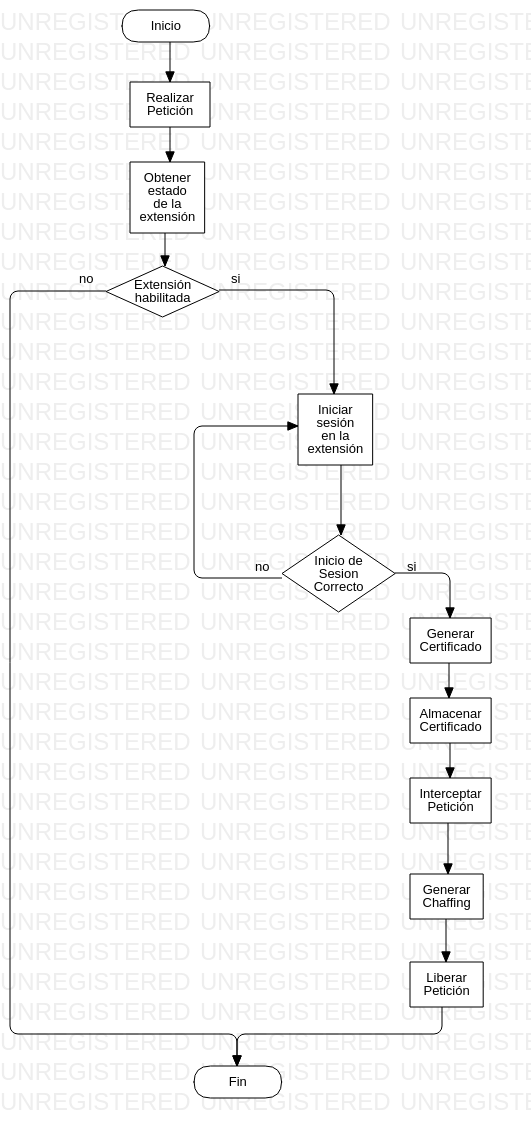
\includegraphics[height=16cm]{./imagenes/Disenio/Componente_1/CI_DF_P1.png}
						\caption{Diagrama de flujo del Componente I.}
					\end{center}
				\end{figure}
				
			    \subsubsection{Descripción diagrama de flujo.}
			        Para el caso de este diagrama se inicia con una petición realizada por el navegador web para luego analizar si la extensión se encuentra activada, en caso de que no no se realiza ninguna acción, pero si si se encuentra se pedirá que se inicie sesión en la extensión con el propósito de generar un certificado válido para el usuario, mas tarde será necesario almacenar este certificado en la extensión y se procederá a interceptar la petición HTTP para modificarla, por lo que se genera el chaffing mediante la combinación de la petición y el certificado para luego liberar la petición modificada al servidor.
				
			\subsection{Diagrama de flujo de datos (DFD).}
			    \begin{figure}[H]
					\begin{center}			        	    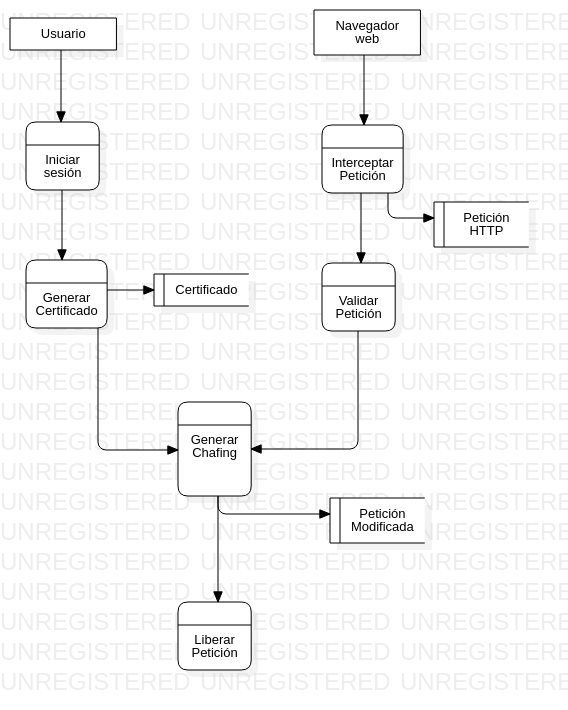
\includegraphics[height=16cm]{./imagenes/Disenio/Componente_1/CI_DFD_P1.png}
						\caption{Diagrama de flujo de datos del Componente I.}
					\end{center}
				\end{figure}
			    
			    \subsubsection{Descripción diagrama de flujo de datos.}
			        En este caso contamos con dos entidades externas, el usuario por una parte debe iniciar sesión para que se pueda generar un \textbf{Certificado} el cual se utilizará para generar el chaffing y por otro lado el Navegador web que intercepta una \textbf{petición HTTP} que de igual manera se utilizará para generar el chaffing. Como resultado de la mezcla de estos dos se genera una \textbf{petición modificada} la cuál mas tarde se liberará para que pueda viajar hacia el servidor.
			   
			\subsection{Diagrama de clases.}
			
    			\begin{figure}[H]
    				\begin{center}	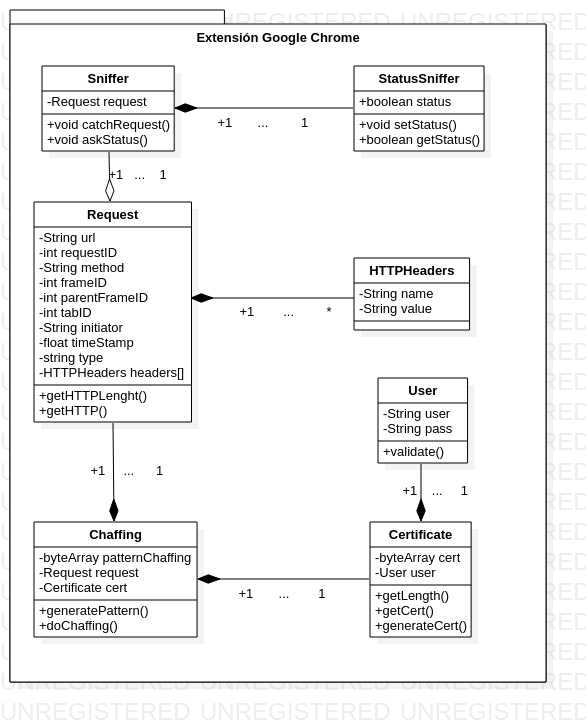
\includegraphics[width=13cm]{./imagenes/Disenio/Componente_1/CI_DC_P1.png}
    				\caption{Diagrama de clases de Componente I.}
    				\end{center}
    			\end{figure}
			    
			    \newpage
			    \subsubsection{Descripción de diagrama de clases}
			    
			    StatusSniffer
			    \begin{enumerate}
    		        \item \textbf{status} : Variable que permite conocer y almacenar el status de la extensión (Habilitada/Deshabilitada).
    		        \begin{enumerate}
    		            \item Tipo de dato: \textbf{boolean}.
    		        \end{enumerate}
    		        Métodos
    		        \begin{enumerate}
    		            \item \textbf{setStatus()}: Se establece el valor del status, True (Está activada la extensión) o False (No está activa la extensión).
    		            \item \textbf{getStatus()}: Se obtiene el valor del status de la extensión, True o False.
    		        \end{enumerate}
			    \end{enumerate}
		        
	            Sniffer
			    \begin{enumerate}
    		        \item \textbf{request} : Variable que almacena los valores de la cabecera HTTP.
    		        \begin{enumerate}
    		            \item Tipo de dato: \textbf{Request}.
    		        \end{enumerate}
    		        Métodos
    		        \begin{enumerate}
    		            \item \textbf{catchRequest()}: Intercepta la petición para obtener los valores de la cabecera.
    		            \item \textbf{askStatus()}: Invoca al método \textit{getStatus()} de la clase StatusSniffer para conocer el status de la extensión.
    		        \end{enumerate}
			    \end{enumerate}
			    
			    Request
			    \begin{enumerate}
    		        \item \textbf{url} : Variable que almacena la URL requerida.
    		        \begin{enumerate}
    		            \item Tipo de dato: \textbf{String}.
    		        \end{enumerate}
    		        \item \textbf{requestID} : Variable que almacena el ID de la petición.
    		        \begin{enumerate}
    		            \item Tipo de dato: \textbf{int}.
    		        \end{enumerate}
    		        \item \textbf{method} : Variable que almacena el tipo de método de la petición, \textit{GET} o \textit{POST}.
    		        \begin{enumerate}
    		            \item Tipo de dato: \textbf{String}.
    		        \end{enumerate}
    		        \item \textbf{frameID} : Variable que almacena el tipo del frame.
    		        \begin{enumerate}
    		            \item Tipo de dato: \textbf{int}.
    		        \end{enumerate}
    		        \item \textbf{parentFrameID} : Variable que almacena el id del frame que envía la petición. 
    		        \begin{enumerate}
    		            \item Tipo de dato: \textbf{int}.
    		        \end{enumerate}
    		        \item \textbf{tabID} : Variable que almacena el ID del tab que toma lugar en la petición.
    		        \begin{enumerate}
    		            \item Tipo de dato: \textbf{int}.
    		        \end{enumerate}
    		        \item \textbf{initiator} : Variable que almacena el origen de la petición.
    		        \begin{enumerate}
    		            \item Tipo de dato: \textbf{String}.
    		        \end{enumerate}
    		        \item \textbf{timeStamp} : Variable que almacena la hora cuando se dispara la petición.
    		        \begin{enumerate}
    		            \item Tipo de dato: \textbf{float}.
    		        \end{enumerate}
    		        \item \textbf{type} : Variable que almacena el tipo de la petición.
    		        \begin{enumerate}
    		            \item Tipo de dato: \textbf{String}.
    		        \end{enumerate}
    		        \item \textbf{headers} : Variable de tipo Array que almacena los headers a ser enviados junto con la petición.
    		        \begin{enumerate}
    		            \item Tipo de dato: \textbf{HTTPHeaders}.
    		        \end{enumerate}
			    \end{enumerate}
			    
			    HTTPHeaders
			    \begin{enumerate}
    		        \item \textbf{name} : Variable que almacena el nombre del header a mandar junto con la petición.
    		        \begin{enumerate}
    		            \item Tipo de dato: \textbf{String}.
    		        \end{enumerate}
    		        \item \textbf{value} : Variable que almacena el contenido del header a enviar junto con la petición.
    		        \begin{enumerate}
    		            \item Tipo de dato: \textbf{String}.
    		        \end{enumerate}
			    \end{enumerate}
			    
			    
			    User
			    \begin{enumerate}
    		        \item \textbf{user} : Variable que permite almacenar el valor del campo nombre de usuario.
    		        \begin{enumerate}
    		            \item Tipo de dato: \textbf{String}. \item Longitud de caracteres: \textbf{20 caracteres}.
    		            \item Restricciones: La cadena sólo puede tener símbolos alfanuméricos 
    		        \end{enumerate}
    		        \item \textbf{pass} : Variable que permite almacenar el valor del campo contraseña.
    		        \begin{enumerate}
    		            \item Tipo de dato: \textbf{String}. \item Longitud de caracteres: \textbf{16 caracteres}.
    		            \item Restricciones: Al menos un \textbf{número} y \textbf{una letra mayúscula}. La cadena sólo puede tener símbolos alfanuméricos.
    		        \end{enumerate}
    		        
    		        Métodos
    		        
    		        \begin{enumerate}
    		            \item validate() : Método que valida que los valores de las variables sean válidos.
    		        \end{enumerate}
			    \end{enumerate}
			        
		        \paragraph{}
	            Certificate
			    \begin{enumerate}
    		        \item \textbf{cert} : Variable que permite almacenar el valor del certificado autentificador.
    		        \begin{enumerate}
    		            \item Tipo de dato: \textbf{byte []}.
    		            \item Longitud: \textbf{40 bytes}.
    		        \end{enumerate}
    		        \item \textbf{user} : Variable que permite almacenar el usuario actual que se está utilizando.
    		        \begin{enumerate}
    		            \item Tipo de dato: \textbf{User}.
    		        \end{enumerate}
    		        
    		        Métodos:
    		        \begin{enumerate}
    		            \item getLenght() : método que devuelve la longitud del certificado.
    		            \item getCert() : método que devuelve el certificado.
    		            \item generateCert() : método que genera el certificado con base a los datos del usuario.
    		        \end{enumerate}
			    \end{enumerate}
			    
			    \paragraph{}
	            Chaffing
			    \begin{enumerate}
    		        \item \textbf{patternChaffing} : Variable que permite almacenar el patrón de \textit{chaffing}.
    		        \begin{enumerate}
    		            \item Tipo de dato: \textbf{byte []}.
    		            \item Longitud: \textbf{HTTP.Lenght() + cert.Lenght()}.
    		        \end{enumerate}
    		        \item \textbf{request} : Variable que permite almacenar la petición HTTP.
    		        \begin{enumerate}
    		            \item Tipo de dato: \textbf{Request}.
    		        \end{enumerate}
    		        \item \textbf{cert} : Variable que permite almacenar el certificado del usuario.
    		        \begin{enumerate}
    		            \item Tipo de dato: \textbf{Certificate}.
    		        \end{enumerate}
    		        
    		        Métodos:
    		        \begin{enumerate}
    		            \item generatePattern() : método que genera el patrón de \textit{chaffing}.
    		            \item doChaffing() : método que realiza el chaffing en la petición HTTP.
    		        \end{enumerate}
			    \end{enumerate}

            \subsection{Diagramas de secuencia.}       
          	
              	\subsubsection{Diagrama de secuencia 1}
                	\begin{figure}[H]
        			    \begin{center} 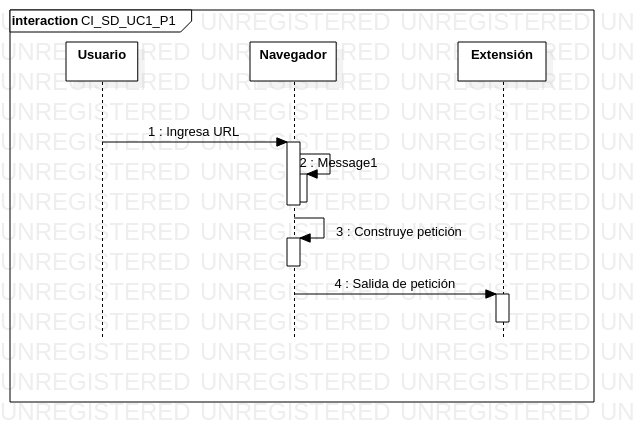
\includegraphics[width=15cm]{./imagenes/Disenio/Componente_1/CI_SD_UC1_P1.png}
        			    \caption[Diagrama de secuencia 1 del Componente I]{Diagrama de secuencia del CI\_CU1. Realizar petición.}
        		        \end{center}
        		    \end{figure}
        		    
        		    \paragraph{Descripción:}
        		    Para realizar una petición, es necesario seguir la siguiente secuencia. Primeramente, el usuario ingresa un URL al navegador, para que este construya la petición que mandará. Una vez que ha construido la petición, la manda a red, pero antes de eso la extensión que actúa como un sniffer, la interceptará.
    		    
    		    
    		     \subsubsection{Diagrama de secuencia 2}
    			    \begin{figure}[H]
    				    \begin{center} 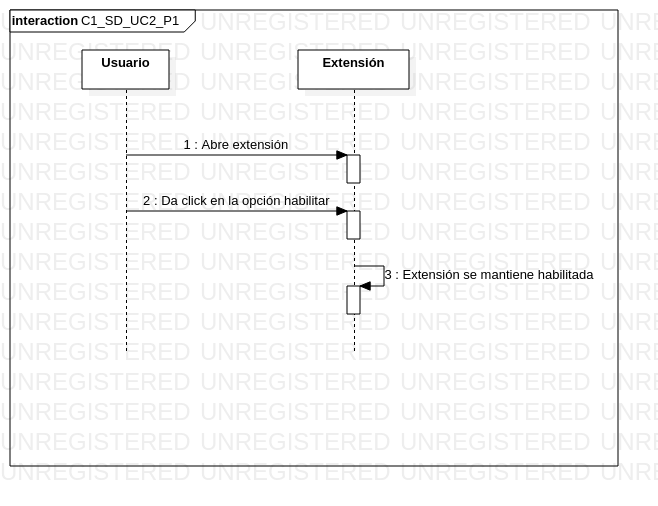
\includegraphics[width=15cm]{./imagenes/Disenio/Componente_1/C1_SD_UC2_P1.png}
    				    \caption[Diagrama de secuencia 2 del Componente I]{Diagrama de secuencia del CI\_CU2. Habilitar extensión.}
    			        \end{center}
    			    \end{figure}
    			    
    			    \paragraph{Descripción:}
    			    Para habilitar la extensión, el usuario necesita primero abrir la extensión. Una vez abierta la extensión, debe de dar click en el botón 'habilitar', para que la extensión ejecute la orden y se mantenga habilitada.
    			    
    			
    			\subsubsection{Diagrama de secuencia 3}
    			    \begin{figure}[H]
    				    \begin{center} 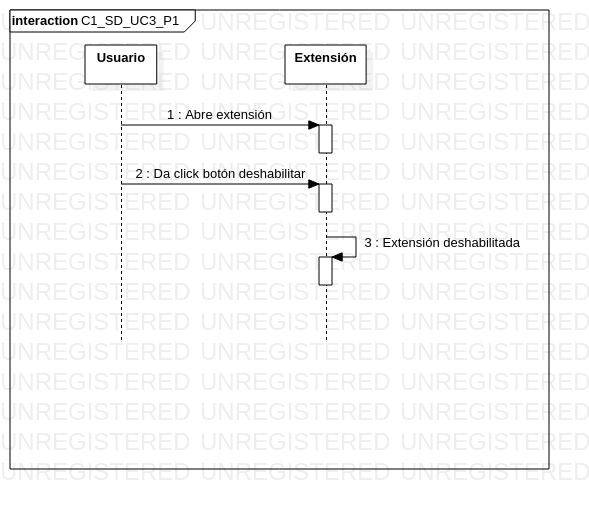
\includegraphics[width=15cm]{./imagenes/Disenio/Componente_1/C1_SD_UC3_P1.png}
    				    \caption[Diagrama de secuencia 3 del Componente I]{Diagrama de secuencia del CI\_CU3. Deshabilitar extensión.}
    			        \end{center}
    			    \end{figure}
    			    
    			    \paragraph{Descripción:}
    			    Para deshabilitar la extensión, el usuario necesita primero abrir la extensión. Una vez abierta la extensión, debe de dar click en el botón ''deshabilitar'', para que la extensión ejecute la orden y se mantenga deshabilitada.
    			   
    			
    			\subsubsection{Diagrama de secuencia 4}
    			    \begin{figure}[H]
    				    \begin{center} 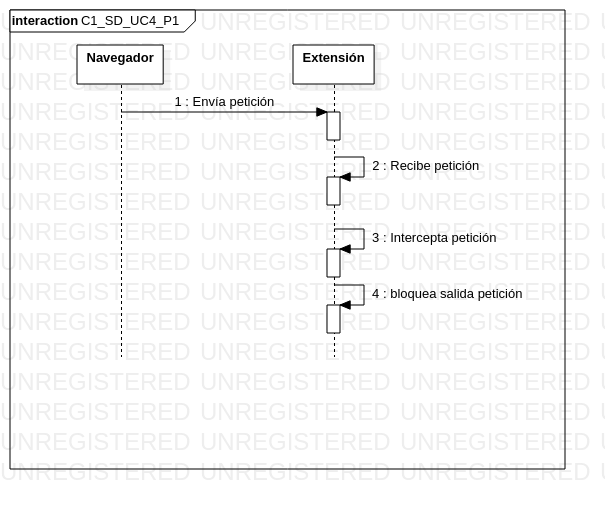
\includegraphics[width=15cm]{./imagenes/Disenio/Componente_1/C1_SD_UC4_P1.png}
    				    \caption[Diagrama de secuencia 4 del Componente I]{Diagrama de secuencia del CI\_CU4. Interceptar petición.}
    			        \end{center}
    			    \end{figure}
    			    
    			    \paragraph{Descripción:}
    			    Una vez que el navegador ha enviado la petición, la extensión la interceptará. Lo primero que hace la extensión para conseguirlo es recibir la petición y bloquear su salida. Con ello la petición jamás saldrá a red y por ende no llegará al servidor.
    			  
              	\subsubsection{Diagrama de secuencia 5.}
        		    \begin{figure}[H]
        				\begin{center}    		    	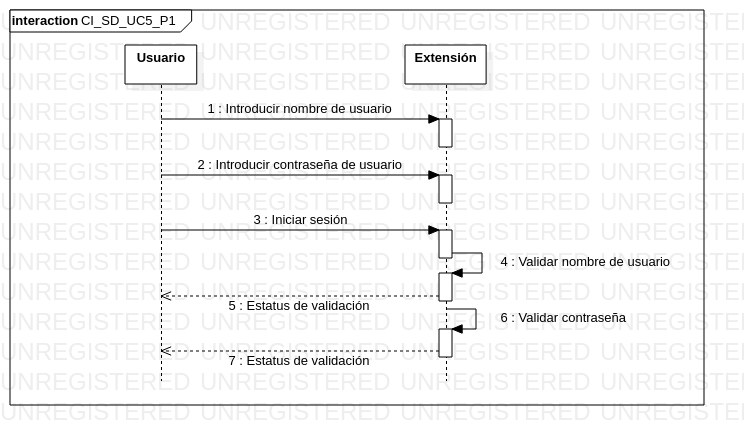
\includegraphics[width=15cm]{./imagenes/Disenio/Componente_1/CI_SD_UC5_P1.png}
        				\caption[Diagrama de secuencia 5 del Componente I]{Diagrama de secuencia del CI\_CU5. Inicio de sesión en la extensión.}
        				\end{center}
        			\end{figure}
        			
        		    \paragraph{Descripción:}
        		    como primeros dos pasos de la secuencia para iniciar sesión en la extensión, el usuario ingresa su nombre de usuario y su contraseña, para después iniciar sesión en la extensión. Una vez que el usuario ha dado la orden de iniciar sesión, la extensión valida el nombre de usuario y la contraseña, retornando un mensaje en caso de que alguno de estos dos valores esté mal. 
    			
    			
    			\subsubsection{Diagrama de secuencia 6.}
        			\begin{figure}[H]
        				\begin{center}    		    	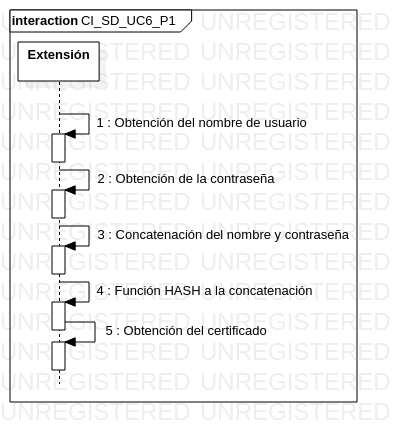
\includegraphics[width=15cm]{./imagenes/Disenio/Componente_1/CI_SD_UC6_P1.png}
        				\caption[Diagrama de secuencia 6 del Componente I]{Diagrama de secuencia del CI\_CU6. Generación del certificado autentificador.}
        				\end{center}
        			\end{figure}
        			
        			\paragraph{Descripción:}
        			Una vez que el usuario ha iniciado sesión, la extensión procede a generar el certificado autentificador. Para ello se obtienen el nombre y la contraseña de usuario para concatenarlos en una única cadena y mandarlos a una función que genere un código HASH (sólo en este prototipo), para después obtener el certificado autentificador.
    			
    			
    			\subsubsection{Diagrama de secuencia 7.}
        			\begin{figure}[H]
        				\begin{center}    		    	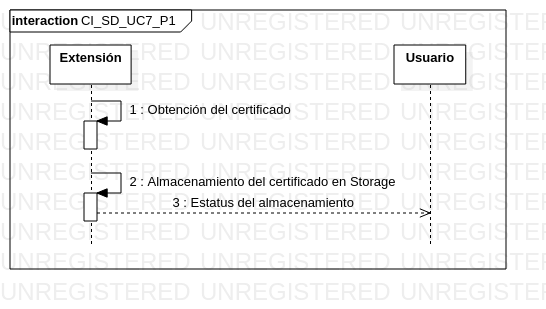
\includegraphics[width=15cm]{./imagenes/Disenio/Componente_1/CI_SD_UC7_P1.png}
        				\caption[Diagrama de secuencia 7 del Componente I]{Diagrama de secuencia del CI\_CU7. Almacenamiento del certificado autentificador.}
        				\end{center}
        			\end{figure}
        			
        			\paragraph{Descripción:}
        			Una vez que se ha generado el código autentificador, es necesario almacenarlo en el Storage de la extensión, para ello la extensión abre una nueva entrada en el Storage y almacena el certificado en ella. Finalmente, la extensión retorna un mensaje del estatus del almacenamiento, para que el usuario se entere si fue exitoso o no.
    			
    			
    			\subsubsection{Diagrama de secuencia 8.}
        			\begin{figure}[H]
        				\begin{center}    		    	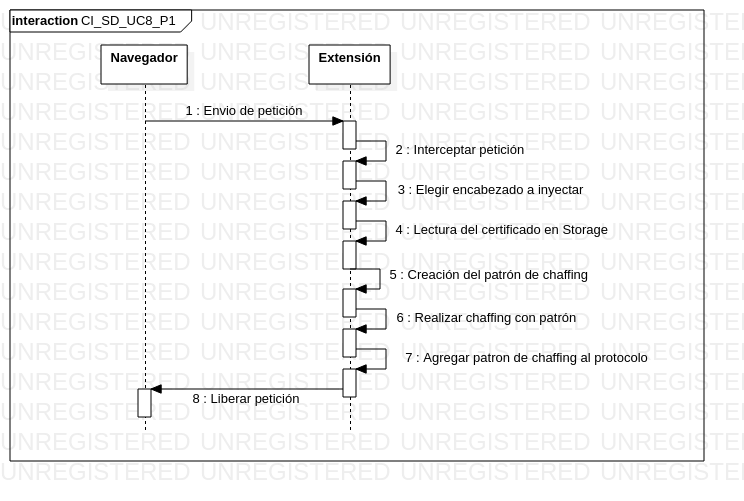
\includegraphics[width=15cm]{./imagenes/Disenio/Componente_1/CI_SD_UC8_P1.png}
        				\caption[Diagrama de secuencia 8 del Componente I]{Diagrama de secuencia del CI\_CU8. Generación del chaffing.}
        				\end{center}
        			\end{figure}
        			
        			\paragraph{Descripción:}
        			Cuando un usuario haga una petición, el navegador enviará dicha petición al servidor correspondiente. Sin embargo, en este momento es cuando la extensión interviene para realizar los pasos necesarios para generar el chaffing. Primeramente, la extensión intercepta la petición para elegir el encabezado a inyectar. Una vez que ha elegido el encabezado, busca obtener el certificado autentificador del Storage, para con base en él, crear el patrón de chaffing con el que se realizará la etapa de chaffing. Finalmente, la extensión agrega el patrón generado a una nueva entrada en el encabezado HTTP interceptado y le manda la señal al navegador para que éste la mande nuevamente. 
    			
    			
    			\subsubsection{Diagrama de secuencia 9.}
        			\begin{figure}[H]
        				\begin{center}    		    	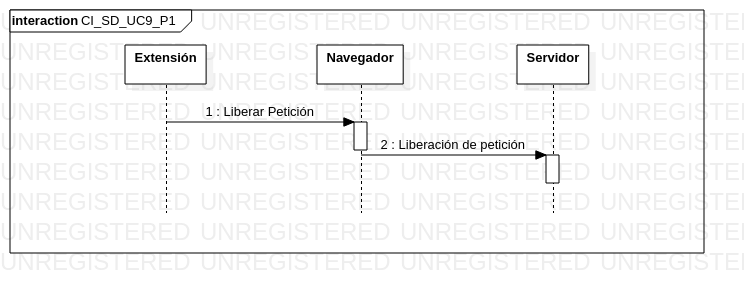
\includegraphics[width=15cm]{./imagenes/Disenio/Componente_1/CI_SD_UC9_P1.png}
        				\caption[Diagrama de secuencia 9 del Componente I]{Diagrama de secuencia del CI\_CU9. Liberación de la petición.}
        				\end{center}
        			\end{figure}
        		
        		    \paragraph{Descripción:}
        		    El navegador una vez que recibe la señal de liberar petición, simplemente tiene que ejecutar su funcionamiento de 'realizar petición' para que ésta salga a red y busque llegar a su destino.
    		
		    \subsection{Diagrama de actividades}
    		    \begin{figure}[H]
    				\begin{center}	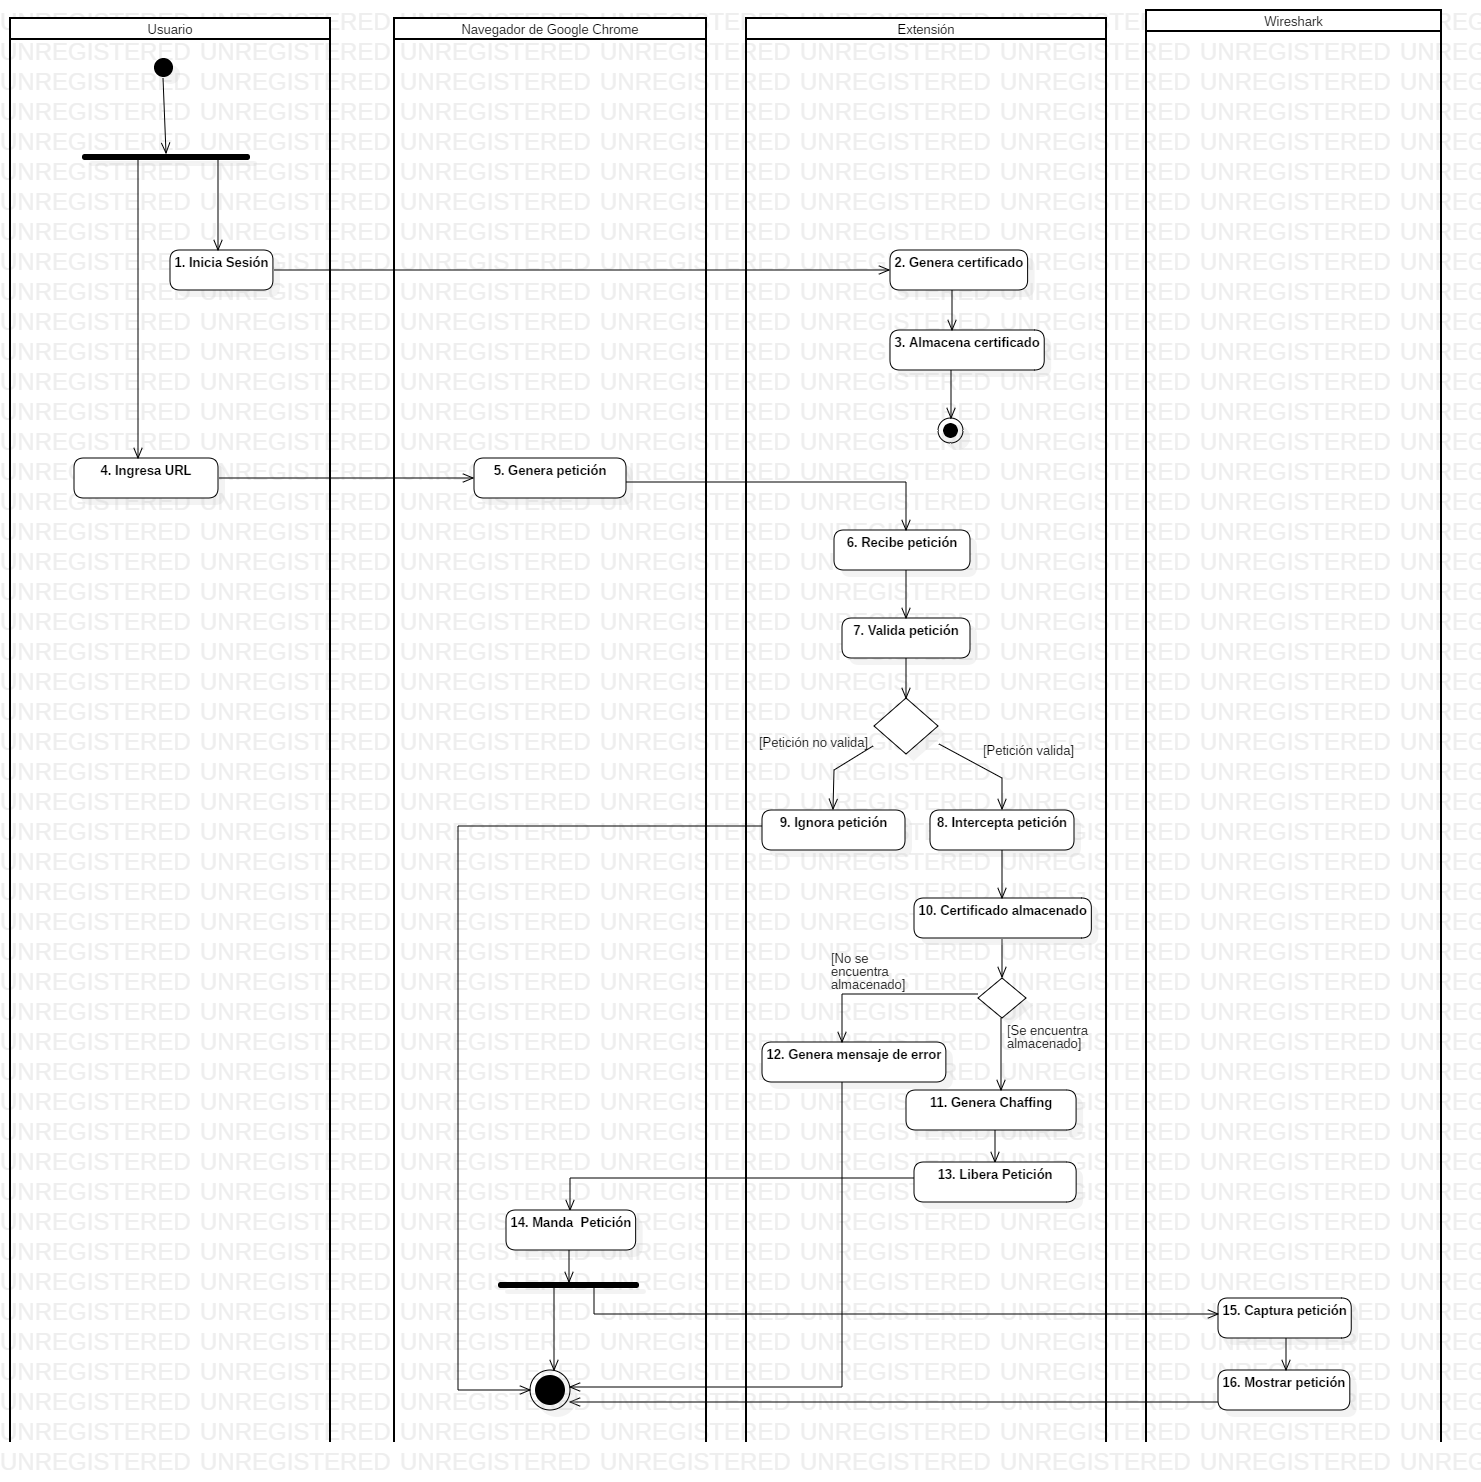
\includegraphics[width=15cm]{./imagenes/Disenio/Componente_1/CI_DA_P1.png}
    					\caption{Diagrama de actividades del Prototipo 2.}
    				\end{center}
    			\end{figure}
    		
        		\subsubsection{Descripción del diagrama de actividades.}
        		El componente cuenta con los siguientes pasos.
            	Uno de los primeros pasos que debe hacer el usuario es iniciar sesión, esto con el fin de generar un certificado de acuerdo a los datos del usuario. Dicho certificado se almacena en el \textbf{Storage} de Google Chrome. \\
            	El otro camino a seguir por el usuario es realizar una búsqueda en el navegador, en la cual el navegador realiza la petición y la extensión recibe la misma. Modificándola siempre y cuando se encuentre un certificado guardado en el Storage. Si este proceso es válido, se genera el proceso de Chaffing y se libera la petición. El servidor se encarga de mandar dicha petición almacenada y en donde el analizador \textit{Wireshark} se encarga de capturar la petición para mostrarla.
			
    		\subsection{Interfaz de usuario.}
                
                \subsubsection{Pantalla Inicial.}
                Esta pantalla es la primer vista que el usuario tiene el sistema. Aparece al darle click a la extensión en su icono correspondiente. En ella, el usuario puede activar y desactivar la extensión para empezar a cachar peticiones, ademas cuenta con un botón de inicio de sesión \textit{(Iniciar Sesión)}, el cual al darle click abrirá la pantalla 'Tab de la extensión' (Figura \ref{fig:CI_Tab}). La Figura \ref{fig:CI_PantallaPrincipal}, muestra como se ve la pantalla inicial.
                
    		    \begin{figure}[H]
    				\begin{center}	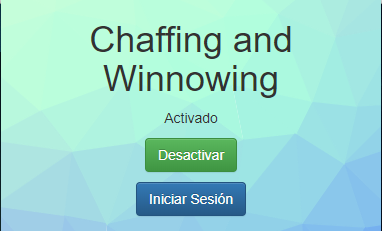
\includegraphics[width=9cm]{./imagenes/Disenio/Componente_1/UI_inicio.PNG}
    					\caption{Pantalla inicial.}
    					\label{fig:CI_PantallaPrincipal}
    				\end{center}
    			\end{figure}
    			
    			\subsubsection{Tab de la extensión.}
    			Esta pantalla es la interfaz que se le brinda al usuario para que inicie sesión y obtenga su certificado autentificador. La Figura \ref{fig:CI_Tab} muestra la pantalla. En ella se aprecian únicamente dos campos para introducir texto ('Ingrese su Usuario' e 'Ingrese su contraseña'), y un botón 'Iniciar Sesión'.
    			  
    		    \begin{figure}[H]
    				\begin{center}	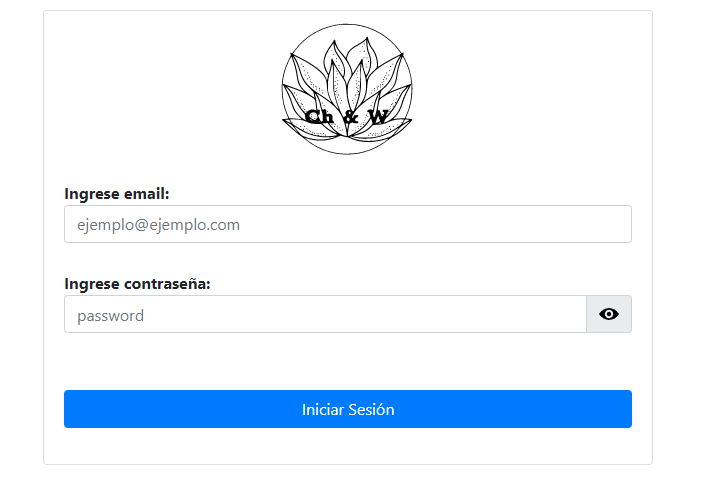
\includegraphics[width=15cm]{./imagenes/Disenio/Componente_1/UI_webpage.PNG}
    					\caption{Tab de la extensión. Permite inicio de sesión}
    					\label{fig:CI_Tab}
    				\end{center}
    			\end{figure}
    			
    			\subsubsection{Mensajes de estado.}
    			Los mensajes de estado, son mensajes que notifican al usuario errores, éxitos o problemas que se presentan al momento de realizar una acción en la extensión. La Figura \ref{fig:UI_certSavedInStorage} muestra el mensaje que se muestra el usuario tras haber guardado el certificado autentificador con éxito en el Storage de la extensión. La Figura \ref{fig:UI_certNotSavedInStorage} notifica al usuario que existió un error al querer guardar el certificado en el Storage de la extensión. Finalmente, la Figura \ref{fig:UI_certNotFound}, muestra que hubo un problema al querer obtener el certificado del Storage de la extensión. 
    			
    			\begin{figure}[H]
    				\begin{center}	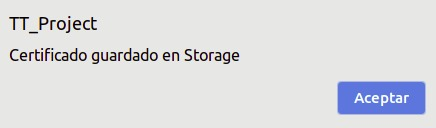
\includegraphics[width=10cm]{./imagenes/Disenio/Componente_1/UI_certSavedInStorage.jpeg}
    					\caption[Mensaje de éxito]{Mensaje de éxito al guardar el certificado en storage de la extensión.}
    					\label{fig:UI_certSavedInStorage}
    				\end{center}
    			\end{figure}
    			
    			\begin{figure}[H]
    				\begin{center}	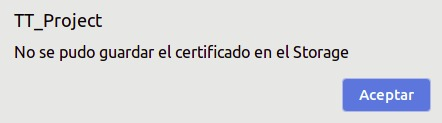
\includegraphics[width=10cm]{./imagenes/Disenio/Componente_1/UI_certNotSavedInStorage.jpeg}
    					\caption[Mensaje de error]{Mensaje de error al guardar el certificado en storage de la extensión.}
    					\label{fig:UI_certNotSavedInStorage}
    				\end{center}
    			\end{figure}
    			
    			\begin{figure}[H]
    				\begin{center}	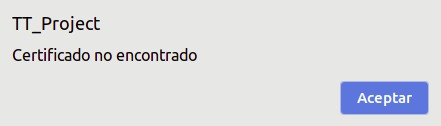
\includegraphics[width=10cm]{./imagenes/Disenio/Componente_1/UI_certNotFound.jpeg}
    					\caption[Mensaje de error en certificado]{Mensaje de error al obtener certificado del storage de la extensión.}
    					\label{fig:UI_certNotFound}
    				\end{center}
    			\end{figure}
			
    	    \subsection{Requisitos de diseño.}
    			   En este apartado, se especificarán los requisitos de diseño para que el prototipo opere de forma correcta, de igualmanera se tiene por entendido que son necesarios los Requisitos del diseño del primer prototipo.
    			   \subsubsection{Requisitos de ejecución de la extensi\'on}
    			        Para poder ejecutar el prototipo dos es necesario contar con todo lo requerido para el prototipo uno y agregarle la interacci\'on con \textbf{jQuery 3.3.1 } y \textbf{Bootstrap} que son dos poderosos frameworks que corren sobre JavaScript y que nos permiten interactuar un poco mejor con el usuario haciendo la interfaz de la extensi\'on más amigable y entendible, estos ya se encuentran insertados en la extensión por lo que no es necesario que el usuario realice acción alguna.
    			        Otros de los requisitos para su ejecución es contar con un \textbf{usuario y contraseña} válidos ya que ser\'an de suma    			    Para deshabilitar la extensión, el usuario necesita primero abrir la extensión. Una vez abierta la extensión, debe de dar click en el botón ''deshabilitar'', para que la extensión ejecute la orden y se mantenga deshabilitada.

 importancia para el correcto funcionamiento del prototipo dos.
    			     \subsubsection{Requisitos para el envío del código autentificador}   
    			        Para este prototipo se considera necesaria los siguientes requisitos de diseño:
    			        \begin{itemize}
    			            \item \textbf{Código Autentificador} Archivo indispenzable en este prototito debido a que sin este es imposible acompletar el proceso.
                            
    			            \item \textbf{Iniciar Sesión} Este botón generará un certificado de prueba y se almacenará en el Storage del navegador Google Chrome. Esto con el fin, que al momento de cachar la petición, la extensión de encargará de inyectar el certificado almacenado modificado con el método \textit{Chaffing} en el encabezado de protocolo HTTP.
    			           
    			        \end{itemize}
    			        \newpage
    			        
    			        
    		\subsection{Algoritmos.}
		        Los algoritmos necesarios para hacer el \textit{chaffing} son expuestos a continuación:\\
                \begin{algorithm}[H]
                    \SetAlgoLined
                    \KwData{requestHTTP, cert}
                    \KwResult{patternChaffing}
                    
                    $lenHTTP \longleftarrow lenght(requestHTTP)$\;
                    $lenCert \longleftarrow lenght(cert)$\;
                    $lenPattern \longleftarrow lenHTTP + lenCert$\;
                    $patternChaffing[lenPattern]$\;
                    $count \longleftarrow 0$\;
                    $y \longleftarrow lenHTTP \% 8$\;
                    
                    \While{$ count < lenCert$}{
                      $x \longleftarrow random \% lenPattern$\;
                      \If{$x <= 0 \quad \&\& \quad x < 8-y \quad \&\& \quad y \quad not \quad 0 $}{
                            $continue$\;
                       }
                       \If{$patternChaffing[x] == 0$}{
                            $patternChaffing[x] \longleftarrow 1$\;
                            $count \longleftarrow count + 1$\;
                       }
                     }
                    $byteControl \longleftarrow 8-y$\;
                    
                    $putFirst(patternChaffing, byteControl)$\;
                    
                    \SetAlgorithmName{Algoritmo}{algoritmo}{Algoritmos}
                    \caption{Generación de patrón de chaffing}
                \end{algorithm}
                
                \newpage
                
                \begin{algorithm}[H]
                    \SetAlgoLined
                    \KwData{requestHTTP, cert, patternChaffing}
                    \KwResult{protocolChaffed}
                    
                    $lenPattern \longleftarrow lenght(PatternChaffing)$\;
                    $protocolChaffed[lenPattern]$
                    $countHTTP \longleftarrow 0$\;
                    $countCert \longleftarrow 0$\;
                    
                    $controlByte \longleftarrow getFirstByte(patternChaffing)$\;
                    
                    $entero \longleftarrow byteToInt(controlByte)$\;
                    
                    $countProtocolChaffed \longleftarrow entero$\;
                    \While{$ countProtocolChaffed < lenPattern$}{
                      \eIf{$protocolChaffed[countProtocolChaffed] == 0$}{
                            $protocolChaffed[countProtocolChaffed] = cert[countCert]$\;
                            $countCert \longleftarrow countCert+1$\;
                       }{
                            $protocolChaffed[countProtocolChaffed] = requestHTTP[countHTTP]$\;
                            $countHTTP \longleftarrow countHTTP+1$\;
                       }
                       $countProtocolChaffed \longleftarrow countProtocolChaffed+1$\;
                    }
                    
                   
                    \SetAlgorithmName{Algoritmo}{algoritmo}{Algoritmos}
                    \caption{Generación de chaffing}
                \end{algorithm}
                
    		   \paragraph{}
    		   Primero vamos a analizar el algoritmo del \textit{patrón de chaffing} con un pequeño ejemplo (utilizaremos datos de variables más cortos); supongamos que nuestro certificado es el siguiente: 
    		    \begin{center}
    		        $C_k = MITZ057abZ251$
    		    \end{center}
    		    y utilizaremos el campo \textit{agent user} del header de la petición, lo cual tendrá lo siguiente:
    		    \begin{center}
    		        $P_{HTTP} = Mozilla5.5/Chrome8.1/Safari$
    		    \end{center}
    		    Entonces, nuestro patrón de chaffing terminará teniendo un tamaño de la longitud de los caracteres de nuestro certificado $+$ la longitud de los datos de la petición HTTP, que es nuestra variable \textit{lenPattern}, y en este caso será de una longitud de 41. A continuación vamos a utilizar un arreglo de banderas de ese tamaño que inicia con 0 todos sus valores, y que al final será nuestro patrón, (variable \textit{patternChaffing}).\\
    		    
    		    La idea es generar posiciones aleatorias dentro del rango del tamaño de \textit{lenPattern}, y poner un 1 en dicha posición si es que hay un 0, en caso de que no se encuentre un 0 se repetirá el procedimiento obteniendo una posición aleatoria diferente, y esto se realizará el mismo número de veces del tamaño de nuestro certificado, para obtener un patrón de combinaciones entre los caracteres. Utilizaremos un contador para conseguir esto, aumentándolo cada vez que se obtenga un número aleatorio válido. En nuestro algoritmo, nuestra variable \textit{x} contiene la posición aleatoria donde se validará si en esa posición se puede poner un 1 o no.\\
    		    
    		    \begin{figure}[H]
        			\begin{center}	                  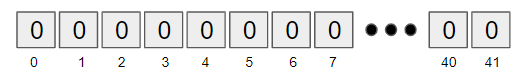
\includegraphics[width=14cm]{./imagenes/Disenio/Componente_1/algorithm1_1.png}
    				\caption{Arreglo del patrón de chaffing}
        			\end{center}
        		\end{figure}
            	
    		    Supongamos, por ejemplo, que el primer número aleatorio que se obtiene es 4, entonces en la posición 4 colocaremos un 1: 
    		    
    		    \begin{figure}[H]
        			\begin{center}	                  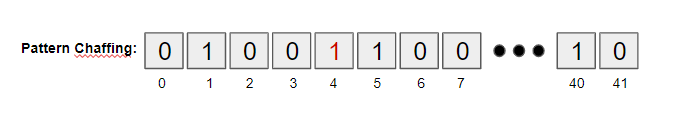
\includegraphics[width=14cm]{./imagenes/Disenio/Componente_1/algorithm1_2.png}
    				\caption{Arreglo del patrón de chaffing después de una iteración}
        			\end{center}
        		\end{figure}
        		
        		Este algoritmo nos permite llenar de unos el número de veces del tamaño de nuestro certificado, lo que nos asegura que cada posición le corresponde a un carácter ya sea del certificado o de la petición a enviar. Supongamos que al terminar este algoritmo, nuestro arreglo queda algo parecido a lo siguiente:
        		
        		\begin{figure}[H]
        			\begin{center}	                  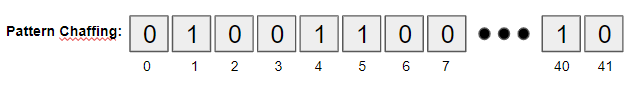
\includegraphics[width=14cm]{./imagenes/Disenio/Componente_1/algorithm1_3.png}
    				\caption{Arreglo del patrón de chaffing final}
        			\end{center}
        		\end{figure}
    		    
    		    El segundo algoritmo realizará el chaff utilizando el patrón generado en el algoritmo anterior, obtendrá el byte de control y a partir de este, comenzará un contador para recorrer todos los bytes del patrón de chaffing, ademas contaremos con otros 2 contadores más: \textit{contCert} que irá recorriendo cada carácter de nuestro certificado, y \textit{countHTTP} que recorrerá los de la petición HTTP. Si en la posición de éste contador se encuentra un 0, entonces quiere decir que debemos de agarrar el siguiente carácter de nuestro certificado, basándonos en el contador del certificado, de la misma manera si se encuentra un 1, se agarrará el siguiente carácter de la petición, y estos se irán concatenando en una nueva cadena (\textit{protocolChaffed}). 
    		    
    		    \begin{figure}[H]
        			\begin{center}	                  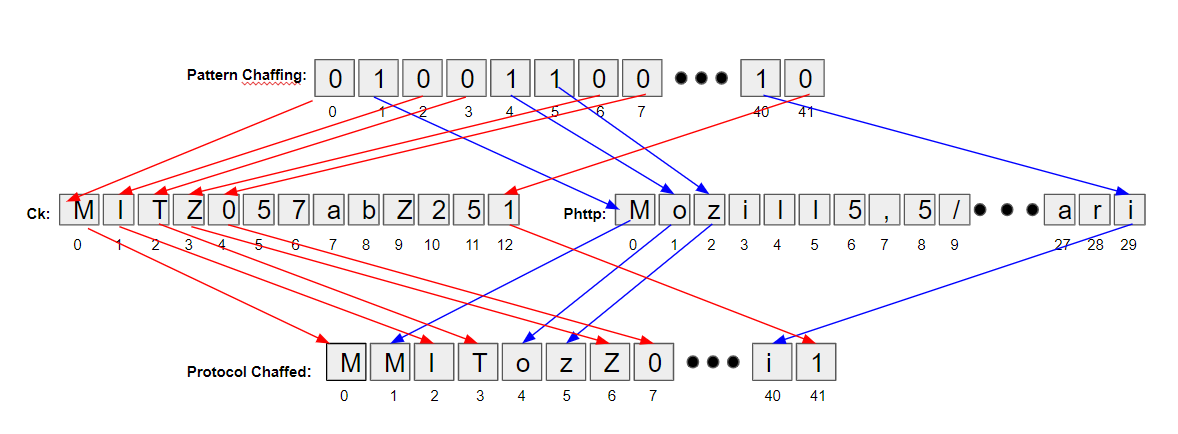
\includegraphics[width=14cm]{./imagenes/Disenio/Componente_1/algorithm2_1.png}
    				\caption{Arreglo chaff final.}
        			\end{center}
        		\end{figure}
    		    
    		    Al final necesitaremos un byte de control que le servirá al servidor saber a partir de donde empezará a realizar el \textit{winnowing}, esto se debe a que dependiendo del tamaño de la petición HTTP y su módulo 8 es donde empezará a checar los 0's y 1's; mandaremos este byte de control al principio de la petición con chaff.\\
    		    
    		    Por último se enviará al servidor el patrón de chaffing junto con el mismo chaff, así podrá saber como realizar el \textit{winowwing} para obtener los datos correspondientes del certificado.


			%INICIO DE DESCRIPCION DE CASOS DE USO DEl COMPONENTE 1
			        
    \chapter{\textcolor{azulescom}{Desarrollo}}
        \section{Componente I.}
            Para verificar que nuestro componente funciona correctamente procedemos a mostrar una prueba del funcionamiento del mismo.\\ Primeramente se necesita iniciar sesión en la extensión, esto con el fin de obtener un certificado y que el mismo se guarde en el storage de Google Chrome. En la prueba iniciamos sesión con los siguientes datos (Figura \ref{fig:InicioDeSesion}): 
    
            \begin{itemize}
                \item \textbf{usuario}: usuarioPrueba
                \item \textbf{contraseña}: usuarioP1234@
            \end{itemize}
    
            \begin{figure}[H]
        		\begin{center}	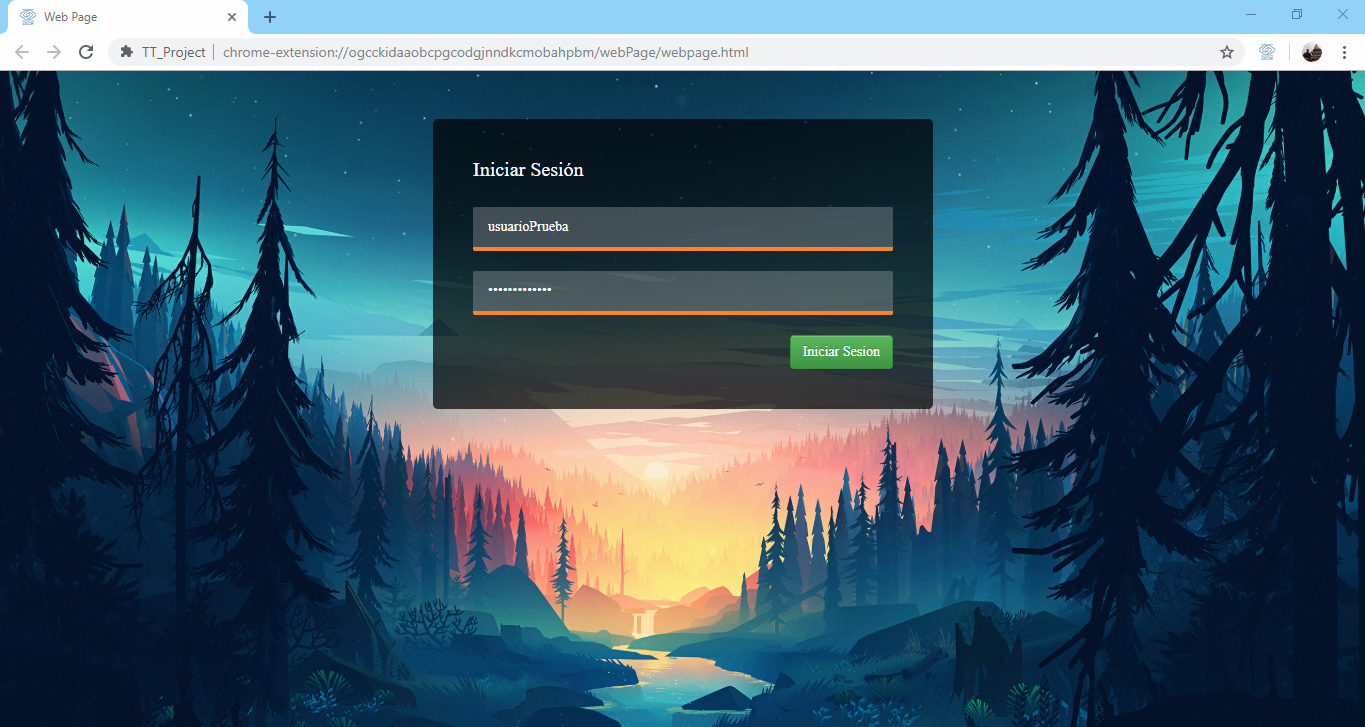
\includegraphics[width=13cm]{./imagenes/Desarrollo/Componente_1/Version1/inicioSesion_prueba.PNG}
        			\caption{Inicio de sesión para la obtención del certificado.}
        		    \label{fig:InicioDeSesion}
        		\end{center}
        	\end{figure}
        	
	        Generando así el siguiente código hash:
        	\begin{center}
        	   \textbf{1408810b7d854a723873e76dbfd989ade608daae}
        	\end{center}
        	Como siguiente paso, este código hash se guarda en el \textit{Storage} de Google Chrome y se da aviso del estado de este procedimiento (Figura \ref{fig:certGuardadoStorage}).
	
        	\begin{figure}[H]
        		\begin{center}	
\includegraphics[width=9cm]{./imagenes/Desarrollo/Componente_1/Version1/certificadoStorage.PNG}
        			\caption{Aviso de guardado del certificado en Storage.}
                    \label{fig:certGuardadoStorage}
        		\end{center}
        	\end{figure}
	
        	Una vez que el certificado se haya guardado con éxito en el \textit{Storage} de Google Chrome, realizamos una búsqueda en Google Chrome, para esta prueba se hizo una petición a un servidor local, montado en \textit{Apache Tomcat} previamente instalado en otra maquina dentro de una red LAN \footnote{Una red de área local o LAN (Local Area Network) es una red de computadoras que abarca un área reducida a una casa, un departamento o un edificio.}. Esta petición será bloqueada por la extensión, como en la Figura \ref{fig:paginaBloqueada}, para inyectar el codigo con \textit{Chaffing} en el protocolo HTTP en el apartado de \textit{headers}.
	
            \begin{figure}[H]
        		\begin{center}	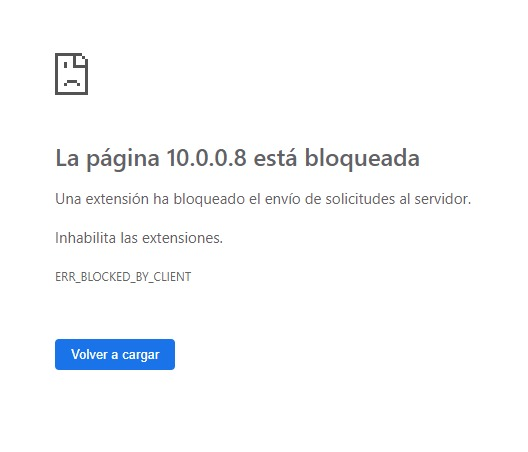
\includegraphics[width=10cm]{./imagenes/Desarrollo/Componente_1/Version1/pageBlocked.jpeg}
        			\caption{Pagina bloqueada del lado del cliente.}
        		    \label{fig:paginaBloqueada}
        		\end{center}
        	\end{figure}
    
            Una vez inyectado el certificado autentificador, se envía la petición con el protocolo modificado al servidor destino. Para verificar que a través de la red se envía la petición modificada se hace uso del analizador de paquetes \hyperref[WiresharkDefinition]{Wireshark}.\\ La Figura \ref{fig:wiresharkAnalizando}, muestra la petición enviada al servidor, donde en el apartado de \textit{Hypertext Transfer Protocol} se observa que en \textbf{Accept} está inyectado el certificado con \textit{Chaffing} y en \textbf{Pattern} está inyectado el patrón realizar el \textit{winnowing} en el servidor (en el siguiente prototipo).
    
            \begin{figure}[H]
        		\begin{center}	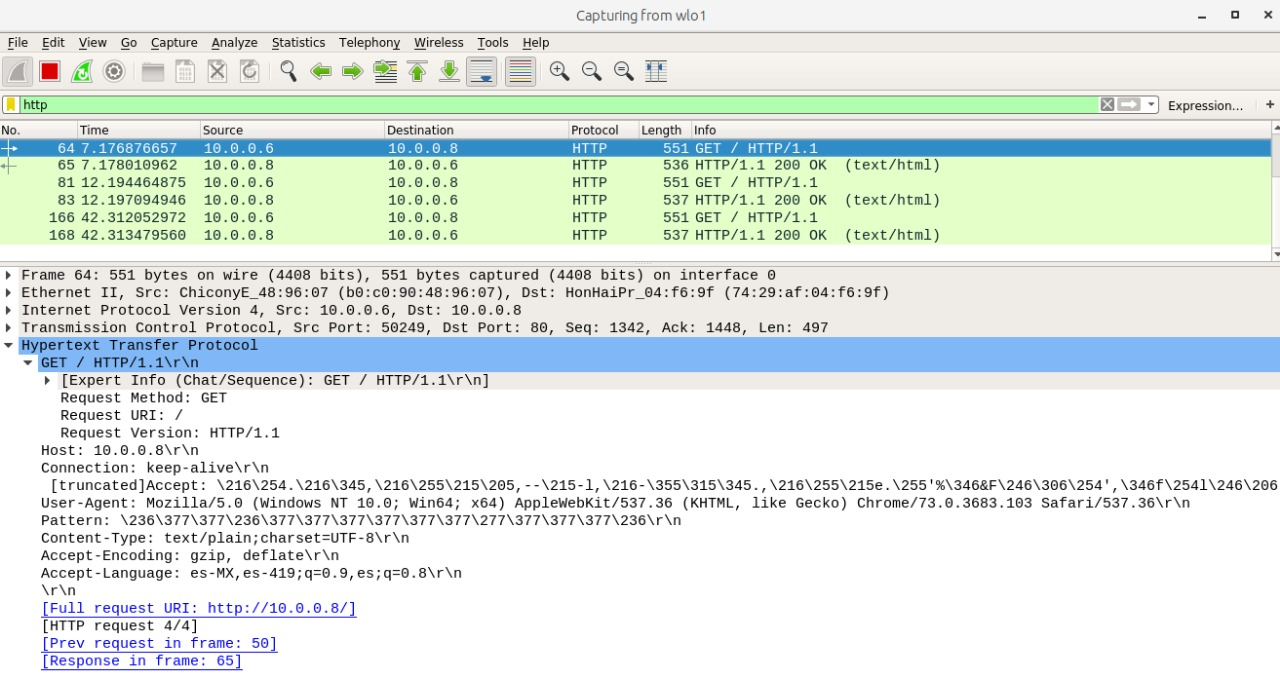
\includegraphics[width=13cm]{./imagenes/Desarrollo/Componente_1/Version1/wiresharkFull.jpeg}
        			\caption{Wireshark analizando en red WI-FI filtrando analisis por \textit{http}.}
        			\label{fig:wiresharkAnalizando}
        		\end{center}
        	\end{figure}
	
        	Para un análisis más específico, se muestra la petición en una herramienta que proporciona wireshark, \textit{Show Packet Bytes...}, la cual muestra el encabezado completo, teniendo una herramienta para seleccionar la codificación del texto (Figura \ref{fig:analisisPeticion}). Nosotros elegimos la codificación ISO8859-1, ya que en ésta nos permite ver de manera legible el encabezado.
	
        	\begin{figure}[H]
        		\begin{center}	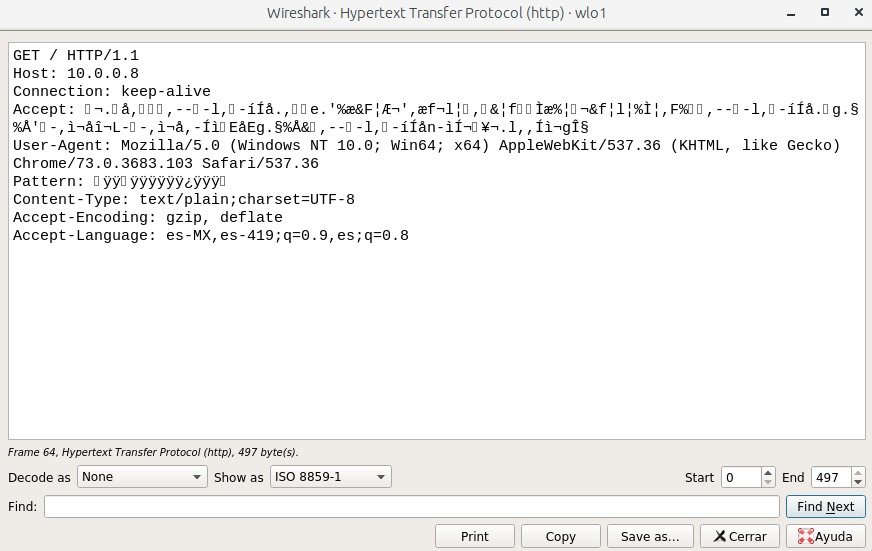
\includegraphics[width=13cm]{./imagenes/Desarrollo/Componente_1/Version1/wiresharkFrame_ISO_header.jpeg}
        			\caption{Análisis de petición en \textit{Show Packet Bytes...}}
        			\label{fig:analisisPeticion}
        		\end{center}
        	\end{figure}
        	
	\newpage
	\chapter{\textcolor{azulescom}{Avances y trabajo por hacer.}}
	    Actualmente hemos desarrollado dos prototipos que son necesarios para conocer el verdadero funcionamiento del sistema, por un lado el prototipo uno nos permite interceptar una petici\'on HTTP con el objetivo de mostrarla para identificar en qué parte de la cabecera agregaremos la parte del código autenticador y c\'omo lo vamos a estructurar y por otro lado el prototipo dos en el cual realizamos el proceso de chaffing del código y su respectivo patr\'on y lo enviaremos por la red a un servicio web, logrando que estos datos lleguen de manera exitosa al otro servidor.
	    Como segunda parte de este trabajo terminal se realizará el análisis y desarrollo de los prototipos 3 y 4 que representan dos de los bloques más importantes de este trabajo terminal, por el lado del prototipo 3 se implementara un servicio web que implementará una API con el propósito de realizar el Winnowing de la petición HTTP modificada por lo que implica una modificación al servidor Apache para que reconozca este tipo de peticiones, por otro lado se implementará un método de cifrado asimétrico mediante RSA para comunicar el patrón resultante de Chaffing de manera segura entre la extensión y el servicio web, de esta manera buscamos autentificar al usuario de manera rápida, eficiente y sencilla para los usuarios. Por otro lado el prototipo 4 consiste en la implementación de un servidor autentificador que será el encargado de crear y  almacenar cada uno de los certificados correspondientes para cada usuario con el fin de que éstos los puedan obtener fácilmente en su extensión logrando que se puedan iniciar múltiples sesiones en diferentes extensiones, siempre cuidando que este certificado se encuentre lo más seguro posible.
	    Como podemos analizar aún nos falta una gran parte de este extenso trabajo pero confiamos en nuestro equipo y en nuestra habilidad para poder resolver todas las problemáticas que se nos presenten en el camino.
	\newpage
	
	\begin{comment}
    	Al terminar este trabajo nos pudimos percatar de todas las nuevas tecnologías que existen y de lo complejo que es ocultar un mensaje no reconocido en las cabeceras HTTP de las peticiones que viajan a través de internet, así como de la complejidad que este trabajo terminal implica ya que al diseñar la arquitectura completa del sistema analizamos cada uno de los bloques que lo iba a conformar y lo complejo que era cada uno de ellos, pero también aprendimos mucho acerca de cuestiones de seguridad en las extensiones de Google Chrome, por otro lado investigamos mucho sobre mecanismos de autentificación y la manera en la que ellos trabajan sobre la red buscando ser lo más seguro posible para todos los usuarios y así mismo confirmamos la necesidad de un método que nos proporcione confidencialidad como lo es Chaffing and Winnowing.
    	
    	A lo largo del desarrollo de los dos primeros prototipos tuvimos muchas dificultades sobre como íbamos a enviar la petición HTTP modificada con el código autentificador y su respectivo patrón sin lograr que cualquier usuario pueda identificarlos fácilmente por lo que realizamos varios cambios a la idea principal de nuestro algoritmo y resultó uno mucho más seguro y mas confidencial de lo que esperábamos. Estamos consientes de que llevamos implementada una pequeña parte de todo el sistema pero tenemos claro cómo lo vamos a realizar y la complejidad que este representa.
    	
    	\chapter{\textcolor{azulescom}{Trabajo a futuro (TT2)}}
    	Como segunda parte de este trabajo terminal se realizará el análisis y desarrollo de los prototipos 3 y 4 que representan dos de los bloques más importantes de este trabajo terminal, por el lado del prototipo 3 se implementara un servicio web que implementará una API con el propósito de realizar el Winnowing de la petición HTTP modificada por lo que implica una modificación al servidor Apache para que reconozca este tipo de peticiones, por otro lado se implementará un método de cifrado asimétrico mediante RSA para comunicar el patrón resultante de Chaffing de manera segura entre la extensión y el servicio web, de esta manera buscamos autentificar al usuario de manera rápida, eficiente y sencilla para los usuarios. Por otro lado el prototipo 4 consiste en la implementación de un servidor autentificador que será el encargado de crear y  almacenar cada uno de los certificados correspondientes para cada usuario con el fin de que éstos los puedan obtener fácilmente en su extensión logrando que se puedan iniciar múltiples sesiones en diferentes extensiones, siempre cuidando que este certificado se encuentre lo más seguro posible.
    	Como podemos analizar todavía nos falta una gran parte de este extenso trabajo pero confiamos en nuestro equipo y en nuestra habilidad para poder resolver todas las problemáticas que se nos presenten en el camino.
    	\newpage
	\end{comment}
    
	%Para agregar una cita en el documento se usa \cite{refKey}, por automático los ordena conforme se van agregando
	\newpage

    \begin{thebibliography}{20}
       
	    \bibitem{refSeguridadWebAguilar}  
		A. Aguilera Hernández (2014, abril 25), Sugerencias de Seguridad para Sitios Web, [En línea]. Disponible: https://www.seguridad.unam.mx/historico/documento/index.html-id=1143. [Último acceso: 15 de febrero del 2019].
	    
	    \bibitem{refRamioAguirre} 
        J. R. Aguirre, \textit{Seguridad Informática y Criptografía}, 2da edición, Madrid, España: Universidad Politécnica de Madrid, 2006.
	    
	    \bibitem{refRivestSeguridad}
		M. Bellare y A. Boldyreva, ''The Security of Chaffing and Winnowing'', California, San Diego, 2015. Disponible: http://citeseerx.ist.psu.edu/viewdoc/download?doi=10.1.\\1.160.4853\&rep=rep1\&type=pdf. [Último acceso: 5 de mayo del 2019].
	
		\bibitem{refCriptology} 
		A. Beutelspacher, \textit{Cryptology}, edición 1994, Washington, Estados Unidos de América: Mathematical Association of America, 1994.
	
	    \bibitem{protocoloHTTP} 
        CCM (2017), El protocolo HTTP, [En línea]. Disponible: https://es.ccm.net/contents/264-el-protocolo-http. [Último acceso: 6 Mayo 2019].

		\bibitem{refSandra} 
        S. Díaz Santiago, ''Generacion De Sucesiones Criptográficamente Fuertes'', tesis de Maestría, División de ciencias básicas e ingeniería, UAM, D.F., México, 2005.
		
		\bibitem{refRoboIdentidad}
		C. C. Espinosa Madrigal (2011, junio 16), Robo de Identidad y Consecuencias Sociales, [En línea]. Disponible: https://www.seguridad.unam.mx/historico/documento/\\index.html-id=16?fbclid=IwAR0u8WAXORvBxZ3H-aMzlBhd-6o7g8ycS88eRu7nY1t1XVtCufhEcQ7hWDs. [Último acceso: 15 de febrero del 2019].
		
		\bibitem{refSHA1}
        T. Fisher (2019), What Is SHA-1 and How Is It Used for Data Verification?, [En línea]. Disponible: https://www.lifewire.com/what-is-sha-1-2626011. [Último acceso: 5 mayo 2019].
		
		\bibitem{refElGranLibro} 
		J. D. Gauchat, \textit{El gran libro de HTML5, CSS3 y Javascript}, 1ra edición, Barcelona, España: MARCOMBO S.A., 2012. 
		
		\bibitem{refEncontrarLuegoAdivinar}
		S.  Goldwasser y S. Micali, ''Probabilistic encryption'', \textit{Journal  of Computer and System Science}, vol. 28, no. 4, pp. 270–299, 1984.
		
		\bibitem{refCryptoJs}
        Google code (2019), crypto-js, [En línea]. Disponible: https://code.google.com/archive/p/crypto-js/. [Último acceso: 5 de mayo del 2019].
		
		\bibitem{refIBMTRIRIGAYear}
        IBM Community (2019), TRIRIGA Wiki Home, [En línea]. DIsponible: 	https://www.ibm.com/developerworks/community/wikis\\
        /home?lang=en\#!/wiki/IBM\%20TRIRIGA1. [Último acceso: 5 mayo 2019].
        
        \bibitem{refIBMTRIRIGA}
        IBM (2019), IBM TRIRIGA Application Platform, [En línea]. Disponible: https://www.ibm.com/support/knowledgecenter/es/SSHEB3\_3.6.0/co m.ibm.tap.doc/sso\_topics/t\_ctr\_authenticate.html. [Último acceso: 5 mayo 2019].
		
	    \bibitem{refFuncionalidadCookies}
		J. Pacheco (2018, julio 18), Entre cookies y privacidad,  Oficina de Seguridad del Internauta, [En línea]. Disponible: https://www.osi.es/es/actualidad/blog/2018/07/18/entre-cookies-y-privacidad. [Último acceso: 5 de mayo del 2019].
		
		\bibitem{ComparisonAuthenticationMethodsResources} 
	    A. Komarova y A. Menshchikov, ''Comparison of Authentication Methods on Web Resources'' en Proceedings of the Second International Scientific Conference ''Intelligent Information Technologies for Industry'', Varna, Bulgaria, 14–16 Septiembre, 2017, pp 106-120.
	    
	    \bibitem{refAONT}
    	J. Larkin, ''Implementation of Chaffing and Winnowing: providing confidentiality without encryption'', tesis de Licenciatura en Ciencias de la Computación, University of Bath Bath, Inglaterra, 2006. [En línea]. Disponible: 
    	https://pdfs.semanticscholar.org/5520/1a43a747f4a3fb554f241c7b7bc76 36b4a07.pdf. [Último acceso: 5 de mayo del 2019].
		
		\bibitem{refCriptografia} 
        A. Maiorano, \textit{Criptografia: Tecnicas De Desarrollo Para Profesionales}, 1ra edición, D.F., México: Alfaomega, 2009.
		
		\bibitem{refChaffingVsEsteganografia} 
    	A. Maurya1, P. Kumar Saini y N. Goel, ''Chaffing and Winnowing without using steganography and encryption technique'', \textit{International Journal of Information Technology and Knowledge Management}, vol. 4, no. 4, pp 515-517, Diciembre, 2011
		
		\bibitem{refHandBookOfAppliedCryptography} 
        A. J. Menezes, P. v. Oorschot y S. Vanstone, \textit{Handbook of Applied Cryptography}, 1ra edición, Florida, Estados Unidos de América: CRC Press, 1996.
		
		\bibitem{refJavaScript} 
		Mozilla (2019, mayo 2), JavaScript. [En línea]. Disponible:
		https://developer.mozilla.org/en-US/docs/Web/JavaScript [Último acceso: 5 de mayo del 2019].
		
		\bibitem{filesystemmozilla}
        Mozilla, (2019, 19 marzo), FileSystem, [En línea]. Disponible: https://developer.mozilla.org/es/docs/Web/API/FileSystem. [Último acceso: 5 de mayo del 2019].
		
		\bibitem{Pressman} 
		R. S. Pressman, \textit{Ingeniería del Software. Un enfoque práctico}, 7ma edición, D.F, México: McGraw-Hill, 2010.
		
		\bibitem{refCryptohraphyWithoutEncryption}
		R. L. Rivest, ''Chaffing and Winnowing: Confidentiality without Encryption'', Laboratorio de ciencias de la computación del MIT, Massachusetts, Estados Unidos de América, 1998.
		
		\bibitem{refSeguridadWeb} 
		A. Romero Mier y Terán y M. A. Vasquéz Martínez (2016, abril 19), Aspectos Básicos de la Seguridad en Aplicaciones Web. [En línea]. Disponble: https://www.seguridad.unam.mx/historico/documento/\\index.html-id=17. [Último acceso: 5 de mayo del 2019].
        
        \bibitem{refCryptography}
	    Universidad Politécnica de Madrid (2004), Criptografía, [En línea]. Disponible: http://www.dma.fi.upm.es/recursos/aplicaciones/matematica\_ discreta/web/aritmetica\_modular/criptografia.html. [Último acceso: 5 de mayo del 2019].
	    
	    \bibitem{opensslmillones}
        VeriSign Inc. (2019), Todo lo que debe saber sobre certificados SSL, [En línea]. Disponible: https://www.verisign.com/es\_LA/website-presence/online/ssl-certificates/index.xhtml. [Último acceso: 5 de mayo del 2019].
        
        \bibitem{refWireshark}
        Wireshark (2019), What is Wireshark?, [En línea]. Disponible: https://www.wireshark.org/docs/wsug\_html\_chunked/Chap\\terIntroduction.html\#ChIntroWhatIs. [Último acceso: 20 abril 2019].
        
        \bibitem{refKerberos}
        Kerberos (2019), Descripción del Kerberos un servicio de autenticación para los sistemas de red abierta, [En línea]. Disponible: https://www.cisco.com/c/es\_mx/support/docs/security-vpn/kerberos/16087-1.html\#whatisit
        
        \bibitem{refCertificados}
        Van Tilborg, Henk C.A, ''Encyclopedia of Cryptography and Security''. \textit{Eindhoven University of Technology The Netherlands}, United States of America, Editorial Springer, 2005, 671 pag. 
        
        \bibitem{refCertificadosElectronicos}
        http://www.itefi.csic.es/sites/default/files/hernandez-encinas/firma-y-certificado-electronico.pdf
        
        \bibitem{refCookies}
        https://www.uv.es/uvweb/universidad/es/politica-privacidad/politica-cookies/son-cookies--1285919089226.html
        
	\end{thebibliography}	

\end{document}
